
%% bare_jrnl_compsoc.tex
%% V1.4a
%% 2014/09/17
%% by Michael Shell
%% See:
%% http://www.michaelshell.org/
%% for current contact information.
%%
%% This is a skeleton file demonstrating the use of IEEEtran.cls
%% (requires IEEEtran.cls version 1.8a or later) with an IEEE
%% Computer Society journal paper.
%%
%% Support sites:
%% http://www.michaelshell.org/tex/ieeetran/
%% http://www.ctan.org/tex-archive/macros/latex/contrib/IEEEtran/
%% and
%% http://www.ieee.org/

%%*************************************************************************
%% Legal Notice:
%% This code is offered as-is without any warranty either expressed or
%% implied; without even the implied warranty of MERCHANTABILITY or
%% FITNESS FOR A PARTICULAR PURPOSE!
%% User assumes all risk.
%% In no event shall IEEE or any contributor to this code be liable for
%% any damages or losses, including, but not limited to, incidental,
%% consequential, or any other damages, resulting from the use or misuse
%% of any information contained here.
%%
%% All comments are the opinions of their respective authors and are not
%% necessarily endorsed by the IEEE.
%%
%% This work is distributed under the LaTeX Project Public License (LPPL)
%% ( http://www.latex-project.org/ ) version 1.3, and may be freely used,
%% distributed and modified. A copy of the LPPL, version 1.3, is included
%% in the base LaTeX documentation of all distributions of LaTeX released
%% 2003/12/01 or later.
%% Retain all contribution notices and credits.
%% ** Modified files should be clearly indicated as such, including  **
%% ** renaming them and changing author support contact information. **
%%
%% File list of work: IEEEtran.cls, IEEEtran_HOWTO.pdf, bare_adv.tex,
%%                    bare_conf.tex, bare_jrnl.tex, bare_conf_compsoc.tex,
%%                    bare_jrnl_compsoc.tex, bare_jrnl_transmag.tex
%%*************************************************************************


% *** Authors should verify (and, if needed, correct) their LaTeX system  ***
% *** with the testflow diagnostic prior to trusting their LaTeX platform ***
% *** with production work. IEEE's font choices and paper sizes can       ***
% *** trigger bugs that do not appear when using other class files.       ***                          ***
% The testflow support page is at:
% http://www.michaelshell.org/tex/testflow/


\documentclass[10pt,journal,compsoc,twoside]{IEEEtran}
%
% If IEEEtran.cls has not been installed into the LaTeX system files,
% manually specify the path to it like:
% \documentclass[10pt,journal,compsoc]{../sty/IEEEtran}

\ifCLASSOPTIONcompsoc
  % IEEE Computer Society needs nocompress option
  % requires cite.sty v4.0 or later (November 2003)
  \usepackage[nocompress]{cite}
\else
  % normal IEEE
  \usepackage{cite}
\fi

\usepackage{enumerate}
\usepackage{latexsym}
\usepackage{amsfonts}
\usepackage{amsmath}
\usepackage{amssymb}
\usepackage{color}
\usepackage{colortbl}
\usepackage{epsfig}
\usepackage{xspace}
\usepackage{graphicx}

\usepackage{subfigure}
\usepackage{balance}
%\usepackage{cite}
\usepackage[english]{babel}



% Some very useful LaTeX packages include:
% (uncomment the ones you want to load)



% *** MISC UTILITY PACKAGES ***
%
%\usepackage{ifpdf}
% Heiko Oberdiek's ifpdf.sty is very useful if you need conditional
% compilation based on whether the output is pdf or dvi.
% usage:
% \ifpdf
%   % pdf code
% \else
%   % dvi code
% \fi
% The latest version of ifpdf.sty can be obtained from:
% http://www.ctan.org/tex-archive/macros/latex/contrib/oberdiek/
% Also, note that IEEEtran.cls V1.7 and later provides a builtin
% \ifCLASSINFOpdf conditional that works the same way.
% When switching from latex to pdflatex and vice-versa, the compiler may
% have to be run twice to clear warning/error messages.






% *** CITATION PACKAGES ***
%

% cite.sty was written by Donald Arseneau
% V1.6 and later of IEEEtran pre-defines the format of the cite.sty package
% \cite{} output to follow that of IEEE. Loading the cite package will
% result in citation numbers being automatically sorted and properly
% "compressed/ranged". e.g., [1], [9], [2], [7], [5], [6] without using
% cite.sty will become [1], [2], [5]--[7], [9] using cite.sty. cite.sty's
% \cite will automatically add leading space, if needed. Use cite.sty's
% noadjust option (cite.sty V3.8 and later) if you want to turn this off
% such as if a citation ever needs to be enclosed in parenthesis.
% cite.sty is already installed on most LaTeX systems. Be sure and use
% version 5.0 (2009-03-20) and later if using hyperref.sty.
% The latest version can be obtained at:
% http://www.ctan.org/tex-archive/macros/latex/contrib/cite/
% The documentation is contained in the cite.sty file itself.
%
% Note that some packages require special options to format as the Computer
% Society requires. In particular, Computer Society  papers do not use
% compressed citation ranges as is done in typical IEEE papers
% (e.g., [1]-[4]). Instead, they list every citation separately in order
% (e.g., [1], [2], [3], [4]). To get the latter we need to load the cite
% package with the nocompress option which is supported by cite.sty v4.0
% and later. Note also the use of a CLASSOPTION conditional provided by
% IEEEtran.cls V1.7 and later.





% *** GRAPHICS RELATED PACKAGES ***
%
\ifCLASSINFOpdf
  % \usepackage[pdftex]{graphicx}
  % declare the path(s) where your graphic files are
  % \graphicspath{{../pdf/}{../jpeg/}}
  % and their extensions so you won't have to specify these with
  % every instance of \includegraphics
  % \DeclareGraphicsExtensions{.pdf,.jpeg,.png}
\else
  % or other class option (dvipsone, dvipdf, if not using dvips). graphicx
  % will default to the driver specified in the system graphics.cfg if no
  % driver is specified.
  % \usepackage[dvips]{graphicx}
  % declare the path(s) where your graphic files are
  % \graphicspath{{../eps/}}
  % and their extensions so you won't have to specify these with
  % every instance of \includegraphics
  % \DeclareGraphicsExtensions{.eps}
\fi
% graphicx was written by David Carlisle and Sebastian Rahtz. It is
% required if you want graphics, photos, etc. graphicx.sty is already
% installed on most LaTeX systems. The latest version and documentation
% can be obtained at:
% http://www.ctan.org/tex-archive/macros/latex/required/graphics/
% Another good source of documentation is "Using Imported Graphics in
% LaTeX2e" by Keith Reckdahl which can be found at:
% http://www.ctan.org/tex-archive/info/epslatex/
%
% latex, and pdflatex in dvi mode, support graphics in encapsulated
% postscript (.eps) format. pdflatex in pdf mode supports graphics
% in .pdf, .jpeg, .png and .mps (metapost) formats. Users should ensure
% that all non-photo figures use a vector format (.eps, .pdf, .mps) and
% not a bitmapped formats (.jpeg, .png). IEEE frowns on bitmapped formats
% which can result in "jaggedy"/blurry rendering of lines and letters as
% well as large increases in file sizes.
%
% You can find documentation about the pdfTeX application at:
% http://www.tug.org/applications/pdftex






% *** MATH PACKAGES ***
%
%\usepackage[cmex10]{amsmath}
% A popular package from the American Mathematical Society that provides
% many useful and powerful commands for dealing with mathematics. If using
% it, be sure to load this package with the cmex10 option to ensure that
% only type 1 fonts will utilized at all point sizes. Without this option,
% it is possible that some math symbols, particularly those within
% footnotes, will be rendered in bitmap form which will result in a
% document that can not be IEEE Xplore compliant!
%
% Also, note that the amsmath package sets \interdisplaylinepenalty to 10000
% thus preventing page breaks from occurring within multiline equations. Use:
%\interdisplaylinepenalty=2500
% after loading amsmath to restore such page breaks as IEEEtran.cls normally
% does. amsmath.sty is already installed on most LaTeX systems. The latest
% version and documentation can be obtained at:
% http://www.ctan.org/tex-archive/macros/latex/required/amslatex/math/





% *** SPECIALIZED LIST PACKAGES ***
%
%\usepackage{algorithmic}
% algorithmic.sty was written by Peter Williams and Rogerio Brito.
% This package provides an algorithmic environment fo describing algorithms.
% You can use the algorithmic environment in-text or within a figure
% environment to provide for a floating algorithm. Do NOT use the algorithm
% floating environment provided by algorithm.sty (by the same authors) or
% algorithm2e.sty (by Christophe Fiorio) as IEEE does not use dedicated
% algorithm float types and packages that provide these will not provide
% correct IEEE style captions. The latest version and documentation of
% algorithmic.sty can be obtained at:
% http://www.ctan.org/tex-archive/macros/latex/contrib/algorithms/
% There is also a support site at:
% http://algorithms.berlios.de/index.html
% Also of interest may be the (relatively newer and more customizable)
% algorithmicx.sty package by Szasz Janos:
% http://www.ctan.org/tex-archive/macros/latex/contrib/algorithmicx/




% *** ALIGNMENT PACKAGES ***
%
%\usepackage{array}
% Frank Mittelbach's and David Carlisle's array.sty patches and improves
% the standard LaTeX2e array and tabular environments to provide better
% appearance and additional user controls. As the default LaTeX2e table
% generation code is lacking to the point of almost being broken with
% respect to the quality of the end results, all users are strongly
% advised to use an enhanced (at the very least that provided by array.sty)
% set of table tools. array.sty is already installed on most systems. The
% latest version and documentation can be obtained at:
% http://www.ctan.org/tex-archive/macros/latex/required/tools/


% IEEEtran contains the IEEEeqnarray family of commands that can be used to
% generate multiline equations as well as matrices, tables, etc., of high
% quality.




% *** SUBFIGURE PACKAGES ***
%\ifCLASSOPTIONcompsoc
%  \usepackage[caption=false,font=footnotesize,labelfont=sf,textfont=sf]{subfig}
%\else
%  \usepackage[caption=false,font=footnotesize]{subfig}
%\fi
% subfig.sty, written by Steven Douglas Cochran, is the modern replacement
% for subfigure.sty, the latter of which is no longer maintained and is
% incompatible with some LaTeX packages including fixltx2e. However,
% subfig.sty requires and automatically loads Axel Sommerfeldt's caption.sty
% which will override IEEEtran.cls' handling of captions and this will result
% in non-IEEE style figure/table captions. To prevent this problem, be sure
% and invoke subfig.sty's "caption=false" package option (available since
% subfig.sty version 1.3, 2005/06/28) as this is will preserve IEEEtran.cls
% handling of captions.
% Note that the Computer Society format requires a sans serif font rather
% than the serif font used in traditional IEEE formatting and thus the need
% to invoke different subfig.sty package options depending on whether
% compsoc mode has been enabled.
%
% The latest version and documentation of subfig.sty can be obtained at:
% http://www.ctan.org/tex-archive/macros/latex/contrib/subfig/




% *** FLOAT PACKAGES ***
%
%\usepackage{fixltx2e}
% fixltx2e, the successor to the earlier fix2col.sty, was written by
% Frank Mittelbach and David Carlisle. This package corrects a few problems
% in the LaTeX2e kernel, the most notable of which is that in current
% LaTeX2e releases, the ordering of single and double column floats is not
% guaranteed to be preserved. Thus, an unpatched LaTeX2e can allow a
% single column figure to be placed prior to an earlier double column
% figure. The latest version and documentation can be found at:
% http://www.ctan.org/tex-archive/macros/latex/base/


%\usepackage{stfloats}
% stfloats.sty was written by Sigitas Tolusis. This package gives LaTeX2e
% the ability to do double column floats at the bottom of the page as well
% as the top. (e.g., "\begin{figure*}[!b]" is not normally possible in
% LaTeX2e). It also provides a command:
%\fnbelowfloat
% to enable the placement of footnotes below bottom floats (the standard
% LaTeX2e kernel puts them above bottom floats). This is an invasive package
% which rewrites many portions of the LaTeX2e float routines. It may not work
% with other packages that modify the LaTeX2e float routines. The latest
% version and documentation can be obtained at:
% http://www.ctan.org/tex-archive/macros/latex/contrib/sttools/
% Do not use the stfloats baselinefloat ability as IEEE does not allow
% \baselineskip to stretch. Authors submitting work to the IEEE should note
% that IEEE rarely uses double column equations and that authors should try
% to avoid such use. Do not be tempted to use the cuted.sty or midfloat.sty
% packages (also by Sigitas Tolusis) as IEEE does not format its papers in
% such ways.
% Do not attempt to use stfloats with fixltx2e as they are incompatible.
% Instead, use Morten Hogholm'a dblfloatfix which combines the features
% of both fixltx2e and stfloats:
%
% \usepackage{dblfloatfix}
% The latest version can be found at:
% http://www.ctan.org/tex-archive/macros/latex/contrib/dblfloatfix/




%\ifCLASSOPTIONcaptionsoff
%  \usepackage[nomarkers]{endfloat}
% \let\MYoriglatexcaption\caption
% \renewcommand{\caption}[2][\relax]{\MYoriglatexcaption[#2]{#2}}
%\fi
% endfloat.sty was written by James Darrell McCauley, Jeff Goldberg and
% Axel Sommerfeldt. This package may be useful when used in conjunction with
% IEEEtran.cls'  captionsoff option. Some IEEE journals/societies require that
% submissions have lists of figures/tables at the end of the paper and that
% figures/tables without any captions are placed on a page by themselves at
% the end of the document. If needed, the draftcls IEEEtran class option or
% \CLASSINPUTbaselinestretch interface can be used to increase the line
% spacing as well. Be sure and use the nomarkers option of endfloat to
% prevent endfloat from "marking" where the figures would have been placed
% in the text. The two hack lines of code above are a slight modification of
% that suggested by in the endfloat docs (section 8.4.1) to ensure that
% the full captions always appear in the list of figures/tables - even if
% the user used the short optional argument of \caption[]{}.
% IEEE papers do not typically make use of \caption[]'s optional argument,
% so this should not be an issue. A similar trick can be used to disable
% captions of packages such as subfig.sty that lack options to turn off
% the subcaptions:
% For subfig.sty:
% \let\MYorigsubfloat\subfloat
% \renewcommand{\subfloat}[2][\relax]{\MYorigsubfloat[]{#2}}
% However, the above trick will not work if both optional arguments of
% the \subfloat command are used. Furthermore, there needs to be a
% description of each subfigure *somewhere* and endfloat does not add
% subfigure captions to its list of figures. Thus, the best approach is to
% avoid the use of subfigure captions (many IEEE journals avoid them anyway)
% and instead reference/explain all the subfigures within the main caption.
% The latest version of endfloat.sty and its documentation can obtained at:
% http://www.ctan.org/tex-archive/macros/latex/contrib/endfloat/
%
% The IEEEtran \ifCLASSOPTIONcaptionsoff conditional can also be used
% later in the document, say, to conditionally put the References on a
% page by themselves.




% *** PDF, URL AND HYPERLINK PACKAGES ***
%
%\usepackage{url}
% url.sty was written by Donald Arseneau. It provides better support for
% handling and breaking URLs. url.sty is already installed on most LaTeX
% systems. The latest version and documentation can be obtained at:
% http://www.ctan.org/tex-archive/macros/latex/contrib/url/
% Basically, \url{my_url_here}.





% *** Do not adjust lengths that control margins, column widths, etc. ***
% *** Do not use packages that alter fonts (such as pslatex).         ***
% There should be no need to do such things with IEEEtran.cls V1.6 and later.
% (Unless specifically asked to do so by the journal or conference you plan
% to submit to, of course. )


% correct bad hyphenation here
\hyphenation{op-tical net-works semi-conduc-tor}

%%%%%%%%%%%%%%%%%%%%%%%%%%%%%%%%%%%%%
%% DO NOT DELETE!!
%%%%%%%%%%%%%%%%%%%%%%%%%%%%%%%%%%%%%
%\usepackage{tikz}
%\usetikzlibrary{trees}

\usepackage{epsfig}
\usepackage{multirow}
\usepackage{url}

%\newcommand{\eq}{\kw{eq}}

\newcommand{\rE}[1]{\kw{\small eHFD}_{#1}}
\newcommand{\rH}[1]{\kw{\small HFD}_{#1}}
\newcommand{\ab}{\allowbreak}

\sloppy
\newcommand{\rtable}[1]{\ensuremath{\mathsf{#1}}}
\newcommand{\ratt}[1]{\ensuremath{\mathit{#1}}}
\newcommand{\at}[1]{\protect\ensuremath{\mathsf{#1}}\xspace}
\newcommand{\myhrule}{\rule[.5pt]{\hsize}{.5pt}}
\newcommand{\oneurl}[1]{\texttt{#1}}
\newcommand{\eat}[1]{}
\newcommand{\tabstrut}{\rule{0pt}{4pt}\vspace{-0.1in}}
\newcommand{\stab}{\vspace{1.2ex}\noindent}
\newcommand{\sstab}{\rule{0pt}{8pt}\\[-1.8ex]}
\newcommand{\match}{\rightleftharpoons}
\newcommand{\eg}{\emph{e.g.,}\xspace}
\newcommand{\ie}{\emph{i.e.,}\xspace}
\newcommand{\true}{\kw{true}}
\newcommand{\kop}{\kw{op}}
\newcommand{\nil}{\kw{nil}}
\newcommand{\Op}{\kw{Op}}
\newcommand{\proofs}{\noindent{\bf Proof sketch:\/ }}
\newcommand{\wrt}{\emph{w.r.t.}\xspace}


%%%%%%%%%%%%%%%%%%%%%%%%%%%%%%%%%%%%%%%%%%%%%%%%%%%%%%%%%%%%%%%%%%%%%%%%%%%%%%
% ALGORITHMS
%%%%%%%%%%%%%%%%%%%%%%%%%%%%%%%%%%%%%%%%%%%%%%%%%%%%%%%%%%%%%%%%%%%%%%%%%%%%%%%
\newcommand{\SELECT}{\mbox{{\bf select}}\ }
\newcommand{\FROM}{\mbox{{\bf from}\ }}
\newcommand{\WHERE}{\mbox{\bf where}\ }
\newcommand{\SUM}{\mbox{{\bf sum}}\ }
\newcommand{\GROUPBY}{\mbox{{\bf group by}}\ }
\newcommand{\HAVING}{\mbox{{\bf having}}\ }
\newcommand{\CASE}{\mbox{{\bf case}}\ }
\newcommand{\END}{\mbox{{\bf end}}\ }
\newcommand{\WHEN}{\mbox{{\bf when}}\ }
\newcommand{\EXISTS}{\mbox{{\bf exists}}\ }
\newcommand{\COUNT}{\mbox{\kw{count}}}
\newcommand{\INSERTINTO}{\mbox{{\bf insert into}}\ }
\newcommand{\UPDATE}{\mbox{{\bf update}}\ }
\newcommand{\SET}{\mbox{{\bf set}}\ }
\newcommand{\IN}{\mbox{{\bf in}}\ }
\newcommand{\If}{\mbox{\bf if}\ }
\newcommand{\Upon}{\mbox{\bf upon}\ }
\newcommand{\Send}{\mbox{\bf send}\ }
\newcommand{\Let}{\mbox{\bf let}\ }
\newcommand{\Call}{\mbox{\bf call}\ }
\newcommand{\Then}{\mbox{\bf then}\ }
\newcommand{\To}{\mbox{\bf to}\ }
\newcommand{\Else}{\mbox{\bf else}\ }
\newcommand{\ElseIf}{\mbox{\bf elseif}\ }
\newcommand{\While}{\mbox{\bf while}\ }
\newcommand{\Begin}{\mbox{\bf begin}\ }
\newcommand{\End}{\mbox{\bf end}\ }
\newcommand{\Do}{\mbox{\bf do}\ }
\newcommand{\Downto}{\mbox{\bf downto}\ }
\newcommand{\Repeat}{\mbox{\bf repeat}\ }
\newcommand{\Until}{\mbox{\bf until}\ }
\newcommand{\For}{\mbox{\bf for}\ }
\newcommand{\Each}{\mbox{\bf each}\ }

\newcommand{\ForEach}{\mbox{\bf for each}\ }
\newcommand{\Or}{\mbox{\bf or}\ }
\renewcommand{\And}{\mbox{\bf and}\ }
\newcommand{\Not}{\mbox{\bf not}\ }
\newcommand{\Break}{\mbox{\bf break}\ }
\newcommand{\Continue}{\mbox{\bf continue}\xspace}
\newcommand{\Return}{\mbox{\bf return}\ }
\newcommand{\Case}{\mbox{\bf case}\ }
\newcommand{\Of}{\mbox{\bf of}\ }
\newcommand{\EndCase}{\mbox{\bf end-case}\ }
\newcommand{\NIL}{\mbox{\em nil}}
\newcommand{\False}{\mbox{\em false}}
\newcommand{\True}{\mbox{\em true}}
\newcommand{\algAND}{{\sc and}\xspace}
\newcommand{\OR}{{\sc or}\xspace}
\newcommand{\NOT}{{\sc not}\xspace}
\newcommand{\kw}[1]{{\ensuremath {\mathsf{#1}}}\xspace}

\newcounter{ccc}
\newcommand{\bcc}{\setcounter{ccc}{1}\theccc.}
\newcommand{\icc}{\addtocounter{ccc}{1}\theccc.}
\newcommand{\checking}{{\mbox{\small\sf Checking}\xspace}}
\newcommand{\preProcessing}{{\mbox{\small\sf preProcessing}\xspace}}
\newcommand{\MCS} {\kw{MCS}}
\newcommand{\templateDB}{{\mbox{\small\sf templateDB}\xspace}}
\newcommand{\ChaseChecking}{{\mbox{\small\sf RandomChecking}\xspace}}
\newcommand{\chase}{{\mbox{\small\sf Chase}\xspace}}
\newcommand{\SAT}{{\mbox{\small\sf SAT}\xspace}}
\newcommand{\kSAT}{{\mbox{\small 3SAT}\xspace}}
\newcommand{\PropCFDSPC}{\kw{Prop{\small CFD\_SPC}}}
\newcommand{\PropCFDSPCU}{\kw{Prop{\small CFD\_SPCU}}}
\newcommand{\UnionEQs}{\kw{UnionEQs}}
\newcommand{\UnionCFDs}{\kw{UnionCFDs}}
\newcommand{\EQ}{\kw{EQ}}
\newcommand{\key}{\kw{key}}
\newcommand{\rep}{\kw{rep}}
\newcommand{\PEQ}{\kw{EQ2CFD}}
\newcommand{\Drop}{\kw{Drop}}
%\newcommand{\Res}{\kw{Res}}

\newcommand{\IND}{{\sc ind}\xspace}
\newcommand{\INDs}{{\sc ind}{\small s}\xspace}
\newcommand{\TGDs}{{\sc tgd}{\small s}\xspace}
\newcommand{\NP}{{\sc np}\xspace}
\newcommand{\DAGs}{{\sc dag}s\xspace}
\newcommand{\NC}{{\sc nc}\xspace}
\newcommand{\coNP}{co{\sc np}\xspace}
\newcommand{\PTIME}{{\sc ptime}\xspace}
\newcommand{\PSPACE}{{\sc pspace}\xspace}
\newcommand{\EXPTIME}{{\sc exptime}\xspace}
\newcommand{\NPSPACE}{{\sc npspace}\xspace}
\newcommand{\dom}{\protect\ensuremath{\mathsf{dom}}\xspace}
\newcommand{\atset}{\protect\ensuremath{\mathsf{attr}}\xspace}
\newcommand{\finatset}{\protect\ensuremath{\mathsf{finattr}}\xspace}
\newcommand{\pvar}{\protect\ensuremath{\mathsf{var\%}}\xspace}
\newcommand{\lLHS}{\protect\ensuremath{\mathsf{{\small LHS}}}\xspace}
\newcommand{\RBR}{\kw{RBR}}
\newcommand{\SQL}{{\sc sql}\xspace}
\newcommand{\XSLT}{{\sc xslt}\xspace}
\newcommand{\DBMS}{{\sc dbms}\xspace}
\newcommand{\ATG}{{\sc atg}\xspace}
\newcommand{\ATGs}{{\sc atg}{\small s}\xspace}
\newcommand{\EBI}{{\sc ebi}\xspace}
\newcommand{\GO}{{\sc go}\xspace}
\newcommand{\VEC}[1]{{\sc vec}(#1)}
\newcommand{\DAG}{{\sc dag}\xspace}
\newcommand{\XQ}{{\sc xq}\xspace}
\newcommand{\XQwc}{{\sc xq}$^{\scriptscriptstyle[*]}$\xspace}
\newcommand{\XQdes}{{\sc xq}$^{\scriptscriptstyle[//]}$\xspace}
\newcommand{\XQfull}{{\sc xq}$^{\scriptscriptstyle[*,//]}$\xspace}
\newcommand{\vect}[1]{$\langle$ #1 $\rangle$}
\newcommand{\sem}[1]{[\![#1]\!]}
\newcommand{\NN}[2]{#1\sem{#2}}
\newcommand{\e}[2]{{\mathit (#1,#2)}}
\newcommand{\ep}[2]{{\mathit (#1,#2)+}}
\newcommand{\brname}{\ensuremath{{\mathsf{N}}}}
\newcommand{\budrel}[1]{\ensuremath{{\brname_{#1}}}}
\newcommand{\budgen}[2]{\ensuremath{Q^\brname_\e{#1}{#2}}}
\newcommand{\budcut}[2]{\ensuremath{Q_\e{#1}{#2}}}
\newcommand{\R}{{\cal R}}
\newcommand{\G}{{\cal G}}
\newcommand{\I}{{\cal I}}
\newcommand{\V}{{\cal V}}
\newcommand{\E}{{\cal E}}
\newcommand{\eop}{\hspace*{\fill}\mbox{$\Box$}}     % End of proof
\newcounter{example}
\renewcommand{\theexample}{\arabic{example}}
\newenvironment{example}{
        \vspace{1.5ex}
        \refstepcounter{example}
        {\noindent\bf Example \theexample:}}{
        \eop\vspace{1.5ex}}
\def\copyrightspace{}
\renewcommand{\ni}{\noindent}
\newcommand{\comlore}[1]{\begin{minipage}{3in}\fbox{\fbox{\parbox[t]{3in}{{\vspace{2mm}\noindent \bf COMM(LORE):~
{ #1}\hfill  END.}}}}\end{minipage}\\}
\newcommand{\comwenfei}[1]{\begin{minipage}{3in}\fbox{\fbox{\parbox[t]{3in}{{\vspace{2mm}\noindent \bf COMM(WENFEI):~
{ #1}\hfill  END.}}}}\end{minipage}\\}
\newcommand{\comshuai}[1]{\begin{minipage}{3in}\fbox{\fbox{\parbox[t]{3in}{{\vspace{2mm}\noindent \bf COMM(SHUAI):~
{ #1}\hfill  END.}}}}\end{minipage}\\}
\newcommand{\nthesection}{\arabic{section}}
\newcounter{theorem}
\renewcommand{\thetheorem}{\arabic{theorem}}
\newcounter{prop}
\renewcommand{\theprop}{\arabic{theorem}}
\newcounter{lemma}
\renewcommand{\thelemma}{\arabic{theorem}}
\newcounter{cor}
\renewcommand{\thecor}{\arabic{theorem}}
\newenvironment{theorem}{\begin{em}
        \refstepcounter{theorem}
        {\vspace{1.5ex} \noindent\bf  Theorem  \thetheorem:}}{
        \end{em}\eop\vspace{1.5ex}} %\hspace*{\fill}\vspace*{1ex}}
\newenvironment{prop}{\begin{em}
        \refstepcounter{theorem}
        {\vspace{1.5ex}\noindent \bf Proposition \theprop:}}{
        \end{em}\eop\vspace{1.5ex}}%\hspace*{\fill}\vspace*{1ex}}
\newenvironment{lemma}{\begin{em}
        \refstepcounter{theorem}
        {\vspace{1ex}\noindent\bf Lemma \thelemma:}}{
        \end{em}\eop\vspace{1ex}} %\hspace*{\fill}\vspace*{1ex}}
\newenvironment{cor}{\begin{em}
        \refstepcounter{theorem}
        {\vspace{1.5ex}\noindent\bf Corollary \thecor:}}{
        \end{em}\eop\vspace{1.5ex}} %\hspace*{\fill}\vspace*{1ex}}
\newcounter{definition}[section]
\renewcommand{\thedefinition}{\nthesection.\arabic{definition}}
\newenvironment{definition}{
        \vspace{1.5ex}
        \refstepcounter{definition}
        {\noindent\bf Definition {\bf \thedefinition}:}}{\eop\vspace{1.5ex}
}
\newcounter{alg}[section]
\renewcommand{\thealg}{\nthesection.\arabic{alg}}
\newenvironment{alg}[1]{
        \refstepcounter{alg}
        {\vspace{1ex}\noindent\bf Algorithm \thealg:\, #1}}{
        \vspace*{1ex}}
\newcounter{arule}
\renewcommand{\thearule}{\arabic{arule}}
\newenvironment{arule}{
        \vspace{0.6ex}
        \refstepcounter{arule}
        {\noindent \em Rule \thearule:}}{
        }
\newcounter{claim}
\renewcommand{\theclaim}{\arabic{claim}}
\newenvironment{claim}{
        \vspace{0.6ex}
        \refstepcounter{claim}
        {\noindent\em Claim \theclaim:}}{%--{ Wenfei Fan}\\
        }
\newenvironment{proof}{
        \vspace{1ex}
        {\noindent\bf Proof:}}{\eop\vspace{1ex}}
\newenvironment{proofS}{
        \vspace{1ex}
        {\noindent\bf Proof:\ }}{\eop\vspace{1ex}}
\newenvironment{property}{
        \vspace{1ex}
        {\noindent\bf Property:}}{\eop\vspace{1ex}}

\newcommand{\RK}[2]{\mbox{(}#1, #2\mbox{)}}

\newenvironment{choice}{\left\{\begin{array}[c]{ll}}{\end{array}\right.}


% Symbol commands

\newcommand{\exa}[2]{{\tt\begin{tabbing}\hspace{#1}\=\+\kill #2\end{tabbing}}}
\newcommand{\ra}{\rightarrow}
\newcommand{\la}{\leftarrow}
\newenvironment{bi}{\begin{itemize}%\vspace{-0.5ex}
        \setlength{\topsep}{0.5ex}\setlength{\itemsep}{0ex}\vspace{0ex}}
        {\end{itemize}\vspace{-1ex}}
\newenvironment{be}{\begin{enumerate}%\vspace{-0.5ex}
        \setlength{\topsep}{0.5ex}\setlength{\itemsep}{0ex}\vspace{-1ex}}
        {\end{itemize}\vspace{-1ex}}
\newcommand{\ei}{\end{itemize}}
\newcommand{\ee}{\end{enumerate}}
\newcommand{\mat}[2]{{\begin{tabbing}\hspace{#1}\=\+\kill #2\end{tabbing}}}
\newcommand{\m}{\hspace{0.05in}}
\newcommand{\ls}{\hspace{0.1in}}
\newcommand{\beqn}{\vspace{-1ex}\begin{eqnarray*}}
\newcommand{\eeqn}{\vspace{-1ex}\end{eqnarray*}}

\newcommand{\INDGreedy}{{\sc IND-Greedy-Step}\xspace}
\newcommand{\FDGreedy}{{\sc FD-Greedy-Step}\xspace}
\newcommand{\INDRepairTup}{{\sc IND-Resolve-Tup}\xspace}
\newcommand{\FDRepairTup}{{\sc FD-Resolve-Tup}\xspace}
\newcommand{\InitEQ}{{\sc Init-EQ}\xspace}
\newcommand{\ResolveEQ}{{\sc Resolve-EQ}\xspace}
\newcommand{\JointFDINDRepair}{{\sc Joint-FD-IND-Repair}\xspace}
\newcommand{\FRP}{{\sc FRP}\xspace}
\newcommand{\class}{\protect\ensuremath{\mathsf{class}}\xspace}
\newcommand{\eq}{\protect\ensuremath{\mathsf{eq}}\xspace}
\newcommand{\cost}{\protect\ensuremath{\mathsf{cost}}\xspace}
\newcommand{\Sim}{\protect\ensuremath{\mathsf{sim}}\xspace}
\newcommand{\dis}{\protect\ensuremath{\mathsf{dis}}\xspace}
\newcommand{\se}{\protect\ensuremath{\mathsf{SE}}\xspace}
\newcommand{\icost}{\protect\ensuremath{\mathsf{inscost}}\xspace}
\newcommand{\mcost}{\protect\ensuremath{\mathsf{mgcost}}\xspace}
\newcommand{\rcost}{\protect\ensuremath{\mathsf{rescost}}\xspace}
\newcommand{\targ}{\protect\ensuremath{\mathsf{targ}}\xspace}
%\newcommand{\ts}{\protect\ensuremath{\mathsf{ts}}\xspace}
\newcommand{\lastcompute}{\protect\ensuremath{\mathsf{lastcompute}}\xspace}
\newcommand{\changed}{\protect\ensuremath{\mathsf{changed}}\xspace}
\newcommand{\new}{\protect\ensuremath{\mathbf{new}}\xspace}
\newcommand{\mtc}{\protect\ensuremath{\mathsf{mtc}}\xspace}
\newcommand{\priQ}{\protect\ensuremath{\mathsf{priQ}}\xspace}
\newcommand{\target}{\protect\ensuremath{\mathsf{target}}\xspace}
\newcommand{\unres}{\protect\ensuremath{\mathsf{unResolved}}\xspace}
\newcommand{\done}{\protect\ensuremath{\mathsf{done}}\xspace}
\newcommand{\pick}{{\sc PickNext}\xspace}
\newcommand{\pickfdfirst}{{\sc PickGreedyFDFirst}\xspace}
\newcommand{\pickfreefd}{{\sc PickGreedyFDFree}\xspace}
\newcommand{\pickgreedy}{{\sc PickGreedy}\xspace}
\newcommand{\pickfd}{{\sc pickNextFD}\xspace}
\newcommand{\rset}{\protect\ensuremath{\mathsf{rset}}\xspace}
\newcommand{\covset}{\protect\ensuremath{\mathsf{coverSet}}\xspace}
\newcommand{\violset}{\protect\ensuremath{\mathsf{violSet}}\xspace}
\newcommand{\attrset}{\protect\ensuremath{\mathsf{attr}}\xspace}
\newcommand{\fattrset}{\protect\ensuremath{\mathsf{finattr}}\xspace}

\newcommand{\pa}{\parallel}
\newcommand{\matchset}{\protect\ensuremath{\mathsf{matchSet}}\xspace}
\newcommand{\bestFix}{\protect\ensuremath{\mathsf{bestFix}}\xspace}
\newcommand{\bestCost}{\protect\ensuremath{\mathsf{bestCost}}\xspace}
\newcommand{\FDFirst}{\protect\ensuremath{\mathsf{FDFirst}}\xspace}
\newcommand{\Null}{\protect\ensuremath{\mathsf{null}}\xspace}
%\renewcommand{\default}[1]{\protect\ensuremath{\mathsf{def}(#1)}\xspace}
\newcommand{\best}[1]{\protect\ensuremath{\mathsf{best}(#1)}\xspace}

\newcommand{\ceq}{=_v}
\newcommand{\AND}{\displaystyle{\bigwedge_{i=1}^{n}}}
\newcommand{\U}[1]{\displaystyle{\bigcup_{#1}}}
\newcommand{\Sm}[1]{\displaystyle{\sum_{#1}}}
\newcommand{\wvec}[1]{\displaystyle{\widehat{#1}}}

\newcommand{\attr}[1]{\protect\ensuremath{\mathsf{#1}}\xspace}

\newcommand{\LA}{\{\!|}
\newcommand{\RA}{|\!\}}
% \newcommand{\tag}[1]{\LA #1\RA}
% \newcommand{\taga}[2]{\LA #1\ \ #2\RA}

\newcommand{\ip}{\Rightarrow_{M}}
\newcommand{\ipu}{\Rightarrow_{M_L}}
\newcommand{\ipp}{\rightarrow_{M}}
\newcommand{\ippu}{\rightarrow_{M_L}}
\newcommand{\inv}{\rightleftharpoons}
\newcommand{\vs}{\vspace{0.1in}}
\newcommand{\Nat}{\mbox{I$\!$N}}


\renewcommand{\L}{{\cal L}}
\newcommand{\md}{\sigma_d}
\newcommand{\inverse}{\sigma_d^{-1}}
\newcommand{\RX}{{\cal X}_R\xspace}
\newcommand{\XP}{{\cal X}\xspace}
\newcommand{\M}{{\cal M}}
\newcommand{\bU}{{\cal U}}
\newcommand{\Ir}{{\cal I}_r}
\newcommand{\B}{{\cal B}}
\renewcommand{\S}{S}
\newcommand{\C}{{\cal C}}
\newcommand{\A}{{\cal A}}
\renewcommand{\v}{\nu}
\renewcommand{\t}{\tau}
\newcommand{\T}{\Theta}
\newcommand{\embedding}{\kw{embedding}}
\newcommand{\expand}{\kw{expand}}
\newcommand{\kstar}{{\sc{star}}\xspace}
\newcommand{\kand}{{\sc{and}}\xspace}
\newcommand{\kor}{{\sc{or}}\xspace}
%\newcommand{\path}{\kw{path}}
\newcommand{\adom}{\kw{adom}}


\newcommand{\Att}{\kw{att}}
\newcommand{\reach}{\kw{reach}}
\newcommand{\partlist}{\kw{part}}
\newcommand{\assg}{\kw{local}}
\newcommand{\qual}{\kw{qual}}
\newcommand{\findpaths}{\kw{findpaths}}
\newcommand{\findpathsDAG}{\kw{findPaths{\sc DAG}}}
\newcommand{\findpathsrnd}{\kw{findPathsRand}}
\newcommand{\findpathsCycle}{\kw{findpathCycle}}
\newcommand{\ordered}{\kw{Ordered}}
\newcommand{\randomordered}{\kw{RandomOrdered}}
\newcommand{\qualityordered}{\kw{QualityOrdered}}
\newcommand{\randmaxind}{\kw{RandomMaxInd}}

%%%%%%%%%%%%%%%%%%%%
% Should be removed
% \newcommand{\sortedseq}{\qualityordered}
% \newcommand{\conflictrepair}{\randomordered}
% \newcommand{\indassign}{\randmaxind}
%%%%%%%%%%%%%%%%%%%%
\newcommand{\topdown}{\kw{topDown}}
\newcommand{\traverse}{\kw{traverse}}
\newcommand{\marked}{\kw{marked}}
\newcommand{\digraph}{{\sc dag}}
\newcommand{\digraphs}{{\sc dag}s}

\newcommand{\dt}{(\C, \v)}
\newcommand{\f}{f_{C \ra C'}}

\newcommand{\imp}{\vdash_{\cal I}}
\newcommand{\Sum}[1]{\displaystyle{\sum_{#1}}}
\newcommand{\MyAnd}[1]{\displaystyle{\bigwedge_{#1}}}

\newcommand{\CFD}{{\sc cfd}\xspace}
\newcommand{\CFDs}{{\sc cfd}{\small s}\xspace}
\newcommand{\CIND}{{\sc cind}\xspace}
\newcommand{\cind}{{\sc cind}}
\newcommand{\CINDs}{{\sc cind}{\small s}\xspace}
\newcommand{\FD}{{\sc fd}\xspace}
\newcommand{\FDs}{{\sc fd}{\small s}\xspace}

\newcommand{\CFDps}{{\small e}{\sc cfd}{\small s}\xspace}

\newcommand{\pCFD}{{\sc cfd$^{p}$}\xspace}
\newcommand{\pCFDs}{{\sc cfd$^{p}$}{\small s}\xspace}
\newcommand{\spCFDs}{{\sc cfd$^{p}$}{\scriptsize s}\xspace}
\newcommand{\sCFDs}{{\sc cfd}{\scriptsize s}\xspace}

\newcommand{\rdms}{{\sc dbms}\xspace}



\newcommand{\pCIND}{{\sc cind$^p$}\xspace}
\newcommand{\pCINDs}{{\sc cind$^p$}{\small s}\xspace}
\newcommand{\spCINDs}{{\sc cind$^p$}{\scriptsize s}\xspace}
\newcommand{\sCINDs}{{\sc cind}{\scriptsize s}\xspace}


\newcommand{\CTGDs}{{\sc ctgd}{\small s}\xspace}
\newcommand{\CGDs}{{\sc cgd}{\small s}\xspace}

\newcommand{\SCFD}{\Sigma_{\kw{cfd^p}}\xspace}
\newcommand{\SCIND}{\Sigma_{\kw{cind^p}}\xspace}


\newcommand{\td}[1]{\widehat{#1}}
\newcommand{\pcdata}{\kw{str}}
\newcommand{\sel}{\kw{sel}}
\newcommand{\ltar}{\ensuremath{L_{\kw{tar}}}}

\newcommand{\ltitle}[1]{\noindent{\large\bf #1}}
\newcommand{\stitle}[1]{\vspace{1.0ex} \noindent{\bf #1}}
\newcommand{\setitle}[1]{\noindent{\em #1}}


\newcommand{\K}{{\cal K}}
\newcommand{\Ka}{{\cal K}_{abs}}
%
\newcommand{\LHS}{\kw{LHS}}
\newcommand{\RHS}{\kw{RHS}}


\renewcommand{\tabstrut}{\rule{0pt}{4pt}\vspace{-0.1in}}
\newcommand{\tabstruct}{\rule{0pt}{8pt}\\[-2ex]}


\newcommand{\tbrule}[1]{{\tt Rule}(#1)}
\newcommand{\frule}[1]{{\tt rule}(#1)}
\newcommand{\lU}{{\bf U} }


\newcommand{\W}{{\bf W}}
\newcommand{\card}[1]{\mid\! #1\!\mid}
\newcommand{\fth}{\hfill $\Box$}


\newcommand{\Inh}[1]{{\it Inh}({\tt #1})}
\newcommand{\Syn}[1]{{\it Syn}({\tt #1})}

\newcommand{\powerset}{{\cal P}}
\newcommand{\determine}{\longrightarrow}
\newcommand{\kleq}{\ll}
\renewcommand{\r}[1]{{\it rule}(#1)}
\newcommand{\MAXSAT}{{\sc maxgsat}\xspace}
\newcommand{\kOr}[1]{\displaystyle{\bigvee_{#1}}}
\newcommand{\kAND}[1]{\displaystyle{\bigwedge_{#1}}}

\newcommand{\batch}{\textsc{BatchDetect}\xspace}
\newcommand{\incre}{{\sc IncDetect}\xspace}

\newcommand{\dsize}{\kw{|D|}}
\newcommand{\noise}{\kw{noise\%}}
\newcommand{\psize}{\kw{|Tp|}}
\newcommand{\numVar}{\kw{Var\%}}
\newcommand{\change}{\kw{|$\Delta$D|}}
\newcommand{\kinserts}{$\kw{|\Delta D^+|}$\xspace}
\newcommand{\kdeletes}{$\kw{|\Delta D^-|}$\xspace}
\newcommand{\Doutputins}{$\kw{|\Delta V^+|}$\xspace}
\newcommand{\Doutputdel}{$\kw{|\Delta V^-|}$\xspace}
\newcommand{\var}{\kw{var}}
\newcommand{\Implic}{\textsc{Implication}\xspace}
\newcommand{\CSP}{\textsc{CSP}\xspace}


%%%%%%%%%%%%%%%%%%%%%%%%%%%%%%%%%%%%%%%%%%
%%%%% Loreto %%%%%%
%%%%%%%%%%%%%%%%%%%%%%%%%%%%%%%%%%%%%%%%%%

\renewcommand{\ni}{\noindent}
\newcommand{\eCFD}{{\small e}{\sc cfd}\xspace}
\newcommand{\eCFDs}{{\small e}{\sc cfd}{\small s}\xspace}
\newcommand{\atns}[1]{\protect\ensuremath{\mathsf{#1}}}



%%%%%%%%%%%%%%%%%%%%%%%%%%%%%%%%%%%%%%%%%%
% Enumerate and Itemize modifications
\newcommand{\OPT}{\protect\ensuremath{\mathsf{OPT}}\xspace}
\newcommand{\kcard}{\kw{card}}
\newcommand{\MAXSC}{{\sc maxss}\xspace}
\newcommand{\MAXGSAT}{{\sc maxgsat}\xspace}

%%%%%%%%%%%%%%%%%%%%%%%%%%%%%%%%%%%%%%%%%%


%%%%%%%%%%%%%%%%%%%%%%%%%%%%%%%%%%%%%%%%%%%%%%%%%%%%%%%%%%%%%%%%%%%%%%%%%%%%%%
% ALGORITHMS
%%%%%%%%%%%%%%%%%%%%%%%%%%%%%%%%%%%%%%%%%%%%%%%%%%%%%%%%%%%%%%%%%%%%%%%%%%%%%%%
%\newcommand{\target}{\protect\ensuremath{\mathsf{target}}\xspace}


\newcommand{\result}{\kw{Result}\xspace}
\newcommand{\kwlog}{\emph{w.l.o.g.}\xspace}
\newcommand{\EMP}[1]{$\kw{emp}_{#1}$}
\newcommand{\opa}[1]{\kw{op}(#1)}
\newcommand{\op}{$\kw{op}$\xspace}
\newcommand{\Enc}[1]{$\kw{enc}_{#1}$}
\newcommand{\bd}[1]{$\textbf{#1}$}

\newcommand{\dblp}{{\sc Dblp}\xspace}
\newcommand{\hosp}{{\sc Hosp}\xspace}
\newcommand{\hcahps}{{\sc hcahps}\xspace}


\begin{document}
%
% paper title
% Titles are generally capitalized except for words such as a, an, and, as,
% at, but, by, for, in, nor, of, on, or, the, to and up, which are usually
% not capitalized unless they are the first or last word of the title.
% Linebreaks \\ can be used within to get better formatting as desired.
% Do not put math or special symbols in the title.
\title{Extending Conditional Dependencies with Built-in Predicates}
%
%
% author names and IEEE memberships
% note positions of commas and nonbreaking spaces ( ~ ) LaTeX will not break
% a structure at a ~ so this keeps an author's name from being broken across
% two lines.
% use \thanks{} to gain access to the first footnote area
% a separate \thanks must be used for each paragraph as LaTeX2e's \thanks
% was not built to handle multiple paragraphs
%
%
%\IEEEcompsocitemizethanks is a special \thanks that produces the bulleted
% lists the Computer Society journals use for "first footnote" author
% affiliations. Use \IEEEcompsocthanksitem which works much like \item
% for each affiliation group. When not in compsoc mode,
% \IEEEcompsocitemizethanks becomes like \thanks and
% \IEEEcompsocthanksitem becomes a line break with idention. This
% facilitates dual compilation, although admittedly the differences in the
% desired content of \author between the different types of papers makes a
% one-size-fits-all approach a daunting prospect. For instance, compsoc
% journal papers have the author affiliations above the "Manuscript
% received ..."  text while in non-compsoc journals this is reversed. Sigh.

\author{Shuai~Ma, %~\IEEEmembership{Senior Member,~IEEE,}
        Liang~Duan,
        Wenfei~Fan, %~\IEEEmembership{Fellow,~ACM,}
        Chunming~Hu, % <-this % stops a space,
        and~Wenguang~Chen %~\IEEEmembership{Fellow,~ACM,}
\IEEEcompsocitemizethanks{\IEEEcompsocthanksitem S. Ma, L. Duan and C. Hu are with the SKLSDE lab, School of Computer Science and Engineering, Beihang University, China.\protect\\
% note need leading \protect in front of \\ to get a newline within \thanks as
% \\ is fragile and will error, could use \hfil\break instead.
E-mail: \{mashuai, duanl, hucm\}@act.buaa.edu.cn.
\IEEEcompsocthanksitem W. Fan is with the RCBD center, Beihang University, China and the School of Informatics, Edinburgh University, UK.\protect\\
E-mail: wenfei@inf.ed.ac.uk.
\IEEEcompsocthanksitem W. Chen is with the Department of Information Management, Peking University, China.\protect\\
E-mail: chenwg@pku.edu.cn.
}% <-this % stops an unwanted space
\thanks{Manuscript received XXX, 2014; revised XXX, 2014.}}

% note the % following the last \IEEEmembership and also \thanks -
% these prevent an unwanted space from occurring between the last author name
% and the end of the author line. i.e., if you had this:
%
% \author{....lastname \thanks{...} \thanks{...} }
%                     ^------------^------------^----Do not want these spaces!
%
% a space would be appended to the last name and could cause every name on that
% line to be shifted left slightly. This is one of those "LaTeX things". For
% instance, "\textbf{A} \textbf{B}" will typeset as "A B" not "AB". To get
% "AB" then you have to do: "\textbf{A}\textbf{B}"
% \thanks is no different in this regard, so shield the last } of each \thanks
% that ends a line with a % and do not let a space in before the next \thanks.
% Spaces after \IEEEmembership other than the last one are OK (and needed) as
% you are supposed to have spaces between the names. For what it is worth,
% this is a minor point as most people would not even notice if the said evil
% space somehow managed to creep in.



% The paper headers
\markboth{IEEE Transactions on Knowledge and Data Engineering,~Vol.~X, No.~X, December~2014}%
{Ma et al.: Extending Conditional Dependencies with Built-in Predicates}
%{Ma \MakeLowercase{\textit{et al.}}: Extending Conditional Dependencies with Built-in Predicates}
% The only time the second header will appear is for the odd numbered pages
% after the title page when using the twoside option.
%
% *** Note that you probably will NOT want to include the author's ***
% *** name in the headers of peer review papers.                   ***
% You can use \ifCLASSOPTIONpeerreview for conditional compilation here if
% you desire.



% The publisher's ID mark at the bottom of the page is less important with
% Computer Society journal papers as those publications place the marks
% outside of the main text columns and, therefore, unlike regular IEEE
% journals, the available text space is not reduced by their presence.
% If you want to put a publisher's ID mark on the page you can do it like
% this:
%\IEEEpubid{0000--0000/00\$00.00~\copyright~2014 IEEE}
% or like this to get the Computer Society new two part style.
%\IEEEpubid{\makebox[\columnwidth]{\hfill 0000--0000/00/\$00.00~\copyright~2014 IEEE}%
%\hspace{\columnsep}\makebox[\columnwidth]{Published by the IEEE Computer Society\hfill}}
% Remember, if you use this you must call \IEEEpubidadjcol in the second
% column for its text to clear the IEEEpubid mark (Computer Society jorunal
% papers don't need this extra clearance.)



% use for special paper notices
%\IEEEspecialpapernotice{(Invited Paper)}



% for Computer Society papers, we must declare the abstract and index terms
% PRIOR to the title within the \IEEEtitleabstractindextext IEEEtran
% command as these need to go into the title area created by \maketitle.
% As a general rule, do not put math, special symbols or citations
% in the abstract or keywords.
\IEEEtitleabstractindextext{%
\begin{abstract}
This paper proposes a natural extension of conditional functional dependencies
(\sCFDs~\cite{CFDs}) and conditional inclusion dependencies
(\sCINDs~\cite{tcs-CINDs}), denoted by \spCFDs and \spCINDs, respectively,
by specifying patterns of data values with $\ne, <, \le, >$ and
$\ge$ predicates.
As data quality rules,  \spCFDs and \spCINDs are able to capture
errors that commonly arise in practice but cannot be detected
by CFDs and CINDs.
We establish two sets of results for central technical
problems associated with  \spCFDs and \spCINDs.
(a) One concerns the satisfiability and implication problems for  \spCFDs and \spCINDs,
taken  separately or together. These are important for, \eg deciding
whether data quality rules are dirty themselves, and for removing
redundant rules.
We show that despite the increased expressive power,
the static analyses of   \spCFDs and \spCINDs retain the same complexity
as their CFDs and CINDs counterparts.
%in the absence of finite domain attributes.
(b) The other concerns validation of  \spCFDs and \spCINDs.
We show that given a set $\Sigma$ of  \spCFDs and \spCINDs on a database $D$,
a set of \SQL queries can be automatically generated
that, when evaluated against $D$, return all tuples in $D$ that
violate some dependencies in $\Sigma$.
\eat{%EAT
We
show that given a set $\Sigma$ of {\pCFDs} and \pCINDs on a database $D$,
a set of \SQL queries can be automatically generated
that, when evaluated against $D$, return all tuples in $D$ that
violate some dependencies in $\Sigma$. Better still,
the \SQL queries are independent of the size and cardinality
of $\Sigma$. }%EAT
We also experimentally verified the efficiency and effectiveness of our \SQL based error detection techniques, using real-life data.
This provides
commercial \DBMS with an immediate capability to detect errors
based on  \spCFDs and \spCINDs.
\end{abstract}

% Note that keywords are not normally used for peerreview papers.
\begin{IEEEkeywords}
Conditional dependencies, built-in predicates, functional dependencies, inclusion dependencies, data quality
\end{IEEEkeywords}
}


% make the title area
\maketitle


% To allow for easy dual compilation without having to reenter the
% abstract/keywords data, the \IEEEtitleabstractindextext text will
% not be used in maketitle, but will appear (i.e., to be "transported")
% here as \IEEEdisplaynontitleabstractindextext when the compsoc
% or transmag modes are not selected <OR> if conference mode is selected
% - because all conference papers position the abstract like regular
% papers do.
%\IEEEdisplaynontitleabstractindextext
% \IEEEdisplaynontitleabstractindextext has no effect when using
% compsoc or transmag under a non-conference mode.



% For peer review papers, you can put extra information on the cover
% page as needed:
% \ifCLASSOPTIONpeerreview
% \begin{center} \bfseries EDICS Category: 3-BBND \end{center}
% \fi
%
% For peerreview papers, this IEEEtran command inserts a page break and
% creates the second title. It will be ignored for other modes.
%\IEEEpeerreviewmaketitle




%%% Local Variables:
%%% mode: latex
%%% TeX-master: "gis18"
%%% End:

\section{introduction}
\label{sec-intro}


\textit{Trajectory tracking} \cite{Lange:Tracking} is a combination of \textit{position tracking} \cite{Wolfson:PositionTracking,Leonhardi:Comparison} and \textit{trajectory simplification} \cite{Lin:Cised,Zhang:Evaluation} in one routine, where \textit{position tracking} is an approach that lets the moving objects database (MOD) server know the current position of a moving object effectively and efficiently, that is, it achieves the desired accuracy of the location information on the server by transmitting as few messages as possible \cite{Leonhardi:Comparison}. Linear dead reckoning (\ldr) \cite{Wolfson:PositionTracking} is such a widely used position tracking method, which is essentially an agreement between a given moving object and a MOD server such that the server could infer the current, excepted position of the moving object whose distance to the actual position of the object is bounded by a user specified threshold;
%
and \textit{trajectory simplification} \cite{Lin:Cised,Zhang:Evaluation} is to approximate a fine trajectory with a coarse one (whose corresponding data points are a subset of the original one), such that the size of the trajectory is reduced under a constrain that the maximum distance of the former to the latter is bounded by a user specified threshold. 
%Linear simplification \cite{Lin:Cised,Zhang:Evaluation} is such an effective and efficient approach that is also widely used in practice.
%
Position tracking and trajectory simplification both are the fundamental technologies of trajectory management and they also share some common target and strategy, \ie, reduce the number of messages or the size of trajectory data by discarding some location information that seems not that important, hence, researchers are trying to combine them in one routine and make it be suitable to run in resource constraint devices.

The authors of \cite{Trajcevski:LDRH} find that the position tracking algorithm \ldr with some tiny modifications is applicable to both track the positions of a moving object and simplify the trajectory built out of these positions. The modified \ldr,  called \ldrh in \cite{Lange:Tracking}, is the first trajectory tracking algorithm that combines position tracking and trajectory simplification into one consistent process. It is concise and efficient, and is suitable for mobile devices. However, it suffers in effectiveness in terms of compression ratio and communication cost, due to the nature of \ldr. 
%
Then, a framework, named the generic remote trajectory simplification (GRTS) \cite{Lange:GRTS,Lange:Tracking}, is developed to improve the effectiveness of trajectory tracking by separate position tracking and trajectory simplification into two sub-processes, where the positions of a moving object is also tracked by \ldr, and these positions are temporarily saved in a buffer and then simplified by some third-party line simplification algorithm. Indeed, it is more effective than \ldrh at a cost of weakening the conciseness and efficiency of \ldrh.
%



\stitle{\todo{Motivations}.}

\ni(1) Trajectory track algorithms are supposed to run in resource-constraint mobile devices, thus, besides good performance of efficiency and effectiveness, they should also be simple and light, \ie having low time and space complexities, otherwise, they are not suitable to run in those mobile devices. In response to these requirements, \ldrh is light, simple and efficient, but not effective; and \grts is effective, but not efficient and light enough. That is, neither of them is the ideal solution for trajectory tracking.
%The emerging of one pass trajectory simplification algorithms. These algorithms can be integrated into grts, however, it is not a natural way to implement a one-pass trajectory tracking algorithm like this way. Acutually, one pass position tracking + one pass trajectory simplification = one pass and effective trajectory tracking algorithm......co-design, like LDRH, yet more effective.


\ni(2) The current works, \ie~\ldrh and \grts, only compress a trajectory or track a moving object in circular areas, \ie the moving object is supposed to locate in a circular taking the expected position of the object as the center. However, in practical, there is a need to track moving objects in other areas, such as strip or rectangular-like areas. \todo{examples and figures of areas,}





\stitle{\todo{Contributions}.}
To the end, we design ways for trajectory tracking in varied areas, including strip and combined areas, and provide three novel one-pass algorithms tracking moving objects effectively and efficiently. 

1. one-pass tracking moving object in circular, citt, effectively and efficiently.

2. one-pass tracking in strips using ped. sitt.
a way that customize region by sed and ped. and implement it in position tracking LDR and trajectory tracking framework GRTS. advantage...

3. one-pass tracking in combined areas using sed and ped. bitt.  
A one-pass trajectory tracking algorithm supporting sed and ped, by a combination cone intersection and sector intersection, \ie co-design of position tracking and trajectory simplification, effective and low time and space complexity, suitable running in resource constraint devices.

4. experiments

\stitle{{Organization}}.
The remainder of the paper is organized as follows:
Section \ref{sec-pre} introduces the basic concepts and the basic HMM method,
Section \ref{sec-method} presents our trajectory simplification aware map-matching method,
Section \ref{sec-exp} reports the experimental results of these methods, followed by related works in Section \ref{sec-related} and conclusion in Section \ref{sec-conclusion}.




%\vspace{-0.5ex}
%\section{Incorporating Built-in Predicates into CFDs}


\section{Extending CFDs with Predicates}
\label{sec-cfd}
%\vspace{-1ex}
%%%%%%%%%%%%%%%%%%%%%%%%%%%%%%%%%



We now define {\em conditional functional dependencies with predicates}, denoted by \pCFDs,
by extending \CFDs~\cite{CFDs} with built-in
predicates ($\ne$, $<$, $\le$, $>$, $\ge$) in addition to equality ($=$).

Consider a relational schema $R$ defined over a finite set of
attributes, denoted by $\attrset(R)$. For each attribute $A \in
\attrset(R)$, its domain is specified in $R$, denoted as $\dom(A)$,
which is either finite (\eg~\at{bool})
or infinite (\eg~\at{string}).
%We use $\fattrset(R)$ to denote
%the set of attributes of $R$ that have a finite domain.
We assume \kwlog that a domain on which $<$, $\le$, $>$ or $\ge$ is defined is totally ordered.


%%%%
\stitle{Syntax}. A \pCFD $\varphi$ on $R$ is a pair
$R(X\ra Y,\ T_p)$, where (1)~$X, Y$ are sets of attributes in
$\attrset(R)$; (2)~$X \ra Y$ is a standard \FD, referred to as the
\FD~{\em embedded in} $\varphi$; and (3)~$T_p$ is a tableau with
attributes in $X$ and $Y$, referred to as the {\em pattern tableau}
of $\varphi$, where for each $A$ in $X \cup Y$ and each tuple $t_p
\in T_p$, $t_p[A]$ is either an unnamed
variable `\_' that draws values from $\dom(A)$, or
`$\op a$', where \op is one of $\{=$, $\ne$,
$<$, $\le$, $>$, $\ge\}$,  and `$a$' is a constant in $\dom(A)$.

If attribute $A$
occurs in both $X$ and $Y$, we use $A_L$ and $A_R$ to indicate the
occurrence of $A$ in $X$ and $Y$, respectively, and we separate the $X$
and $Y$ attributes in a pattern tuple with `$\pa$'.
We simply write $\varphi$ as $(X \ra Y,\ T_p)$ when $R$ is clear from the
context, and denote $X$ as $\mbox{\LHS}(\varphi)$ and $Y$ as
$\mbox{\RHS}(\varphi)$, respectively.



%\vspace{-1ex}
\begin{example}
The dependencies \kw{cfd_1}--\kw{cfd_3} and \kw{pfd_1}--\kw{pfd_4}
that we have seen in Example~\ref{exa-motivation} can all be expressed as \pCFDs.  Some of these \pCFDs
are illustrated in Fig.~\ref{fig-pcfd}, in which $\varphi_1$ is for \FD\ \kw{cfd_2},
$\varphi_2$ is for \CFD\ \kw{cfd_3}, $\varphi_3$ is for \kw{pfd_2},
and $\varphi_4$ is for \kw{pfd_4}, respectively.
\end{example}
\vspace{-1ex}


\stitle{Semantics}. Consider \pCFD $\varphi$ =
$R(X\ra Y$, $T_p)$, where $T_p = \{t_{p_1}, \ldots, t_{p_k}\}$.

A data tuple $t$ of $R$ is said to {\em match} $\LHS(\varphi)$,
denoted by $t[X] \asymp T_p[X]$, if {\em for each tuple
$t_{p_i}$ ($i\in[1, k]$) in $T_p$} and {\em each attribute $A$} in $X$, either
(a)  $t_{p_i}[A]$ is the wildcard `\_' (which matches any value
in $\dom(A)$),  or
(b) $t[A]\ \op a$ if $t_{p_i}[A]$ is `$\op a$', where
the operator $\op$ ($=$, $\ne$,
$<$, $\le$, $>$ or $\ge$) is interpreted by its standard
semantics. Similarly, the notion that $t$ {\em matches} $\RHS(\varphi)$
is defined, denoted by $t[Y] \asymp T_p[Y]$.


Intuitively, each pattern tuple $t_{p_i}$ ($i\in[1, k]$) specifies a condition via
$t_{p_i}[X]$, and $t[X] \asymp T_p[X]$ if
 $t[X]$ satisfies the {\em conjunction} of all these conditions.
Similarly, $t[Y] \asymp T_p[Y]$ if $t[Y]$ matches all the patterns
specified by $t_{p_i}[Y]$ for all pattern tuples $t_{p_i}$ in $T_p$.

An instance $I$ of $R$ {\em satisfies} the \pCFD $\varphi$, denoted
by $I \models \varphi$, if  for {\em each pair} of tuples $t_1, t_2$
in $I$, if $t_1[X] = t_2[X] \asymp T_p[X]$, then
$t_1[Y] = t_2[Y] \asymp T_p[Y]$.  That is, if $t_1[X]$ and $t_2[X]$
are equal and in addition, they both match the pattern tableau
$T_p[X]$, then $t_1[Y]$ and $t_2[Y]$ must also be equal to each
other and they both match the pattern tableau $T_p[Y]$.

Observe that $\varphi$ is imposed only on the subset of tuples in
$I$ that match $\LHS(\varphi)$, rather than on the entire $I$. For
all tuples $t_1, t_2$ in this subset, if $t_1[X] = t_2[X]$, then
(a)~$t_1[Y] = t_2[Y]$, \ie~the semantics of the embedded \FDs is
enforced; and (b)~$t_1[Y] \asymp T_p[Y]$, which assures that the
{\em constants} in $t_1[Y]$ match the {\em constants} in $t_{p_i}[Y]$
for all $t_{p_i}$ in $T_p$. Note that here tuples $t_1$ and $t_2$ can
be the same.



An instance $I$ of $R$ satisfies a set $\Sigma$ of \pCFDs,
denoted by $I\models\Sigma$, if $I\models\varphi$ for {\em each}
\pCFD $\varphi$ in $\Sigma$.


%%%%%%%%%%%%%%%%%%%%%pCIND exmaple%%%%%%%%%%%%
\begin{figure*}[tbh!]
\vspace{1ex}
\begin{center}
(1) $\psi_1$ = (\at{item}\lbrack\at{state}; $\at{type}\rbrack$
$\subseteq$ \at{tax}\lbrack\at{state}; $\NIL\rbrack$, \ $T_{1}$), \\
\sstab (2) $\psi_2$ = (\at{item}\lbrack\at{state}; $\at{type,
state}\rbrack$ $\subseteq$ \at{tax}\lbrack\at{state};
$\at{rate}\rbrack$, \ $T_{2}$)\\ \sstab $T_1$: \begin{tabular}{c||c}
\at{type} &  \kw{ nil} \\ \hline
 $\ne$ art  &  \\
\end{tabular}
\hspace{10ex}
$T_2$:
\begin{tabular}{c | c || c}
\at{type} & \at{state} & \at{rate} \\ \hline
 $\ne$ art  & $=$ DL & $=$ 0 \\
\end{tabular}
\end{center}
\vspace{-2ex} \caption{Example \pCINDs} \label{fig-pcind}
\vspace{-3ex}
\end{figure*}
%%%%%%%%%%%%%%%%%%%%%%%%%%%%%


\vspace{-1ex}
\begin{example}
The instance $D_0$ of
Fig.~\ref{fig-instance} satisfies $\varphi_1$ and $\varphi_2$ of
Fig.~\ref{fig-pcfd}, but neither $\varphi_3$ nor
$\varphi_4$. Indeed, tuple $t_3$ violates (\ie~does not satisfy)
$\varphi_3$, since
$t_3[\at{sale}]$ = `F' {\em and} $20 < t_3[\at{price}] \le 40$,
but $t_3[\at{shipping}]$ is 20 instead of $6$.
Note that $t_3$ matches $\LHS(\varphi_3)$ since it satisfies
the condition specified by the {\em conjunction}
of the pattern tuples in $T_3$.
Similarly, $t_1$ violates $\varphi_4$, since
$t_1[\at{sale}]$ = `T' but $t_1[\at{price}] > 9.99$.
Observe that while it takes two tuples
to violate a standard \FD, a single tuple may violate a
\pCFD.
\end{example}
\vspace{-1.5ex}






\stitle{Special cases.}~(1) A standard \FD $X\ra Y$~\cite{AbHuVi1995} can
be expressed as a \CFD $(X\ra Y,\ T_p)$ in which $T_p$ contains a
single tuple consisting of `\_' only, without constants. (2) A
\CFD $(X\ra Y,\ T_p)$~\cite{CFDs} with
$T_p = \{t_{p1},\ldots, t_{pk}\}$ can be
expressed as a set $\{\varphi_1,\ldots,\varphi_k\}$ of
\pCFDs such that for each $i\in [1, k]$, $\varphi_i$ = $(X\ra Y,\
T_{p_i})$, where $T_{p_i}$ contains the pattern tuple $t_{p_i}$ of
$T_p$ only, defined with equality $(=)$ only.
For example, $\varphi_1$ and $\varphi_2$ in
Fig.~\ref{fig-pcfd} are \pCFDs representing \FD $\kw{cfd_2}$
and \CFD $\kw{cfd_3}$ in Example~\ref{exa-motivation}, respectively.
Note that all data quality
rules in~\cite{CM08,divesh08} can be expressed as
\pCFDs.



\section{Extending CINDs with Predicates}
\label{sec-cind}
%\vspace{-1ex}



Similar to \pCFDs, we define {\em conditional inclusion dependencies with predicates}, denoted by \pCINDs,
by extending \CINDs~\cite{tcs-CINDs} with built-in predicates ($\ne$, $<$, $\le$, $>$, $\ge$) in addition to equality ($=$).
%
Consider two relational schemas $R_1$ and $R_2$.

%\vspace{-0.5ex}
\stitle{Syntax.} A \pCIND $\psi$ is a pair
$(R_1[X;\ X_p] \subseteq R_2[Y;\ Y_p],\ T_p)$, where (1)~$X, X_p$
and  $Y, Y_p$ are lists of attributes in $\attrset(R_1)$ and
$\attrset(R_2)$, respectively; (2)~$R_1[X] \subseteq R_2[Y]$ is a
standard \IND, referred to as the \IND\ {\em embedded} in $\psi$;
and (3)~$T_p$ is a tableau, called the {\em pattern tableau} of
$\psi$ defined over attributes $X_p\cup Y_p$, and for each $A$ in
$X_p$ or $Y_p$ and each pattern tuple $t_p \in T_p$, $t_p[A]$ is either
an unnamed variable `\_' that draws values from $\dom(A)$, or
`\op a', where \op is one of $=, \ne, <, \le, >, \ge$ and `a' is a
constant in $\dom(A)$.

 We denote $X \cup X_p$ as $\LHS(\psi)$, $Y \cup Y_p$ as $\RHS(\psi)$, and
separate the $X_p$ and $Y_p$ attributes in a pattern tuple with
`$\pa$'. We also use \kw{nil} to denote an {\em empty} list. \eat{Relation
$R_1$ (resp. $R_2$) is called the \LHS (resp. \RHS) relation of
\pCIND $\psi$.}


%In addition, we also assume a finite domain contains at least two elements.

\vspace{-0.5ex}
\begin{example}
\label{exam-pcind} Figure~\ref{fig-pcind} shows two example \pCINDs:
$\psi_1$ expresses the $\kw{pind}_1$ in Example~\ref{exa-motivation},
and $\psi_2$ refines $\psi_1$ by stating that for any \at{item}
tuple $t_1$, if its \at{type} is not art and its \at{state} is DL,
then there must be a \at{tax} tuple $t_2$ such that its \at{state}
is DL and \at{rate} is $0$, \ie~$\psi_2$ assures that the sale tax
rate in Delaware is 0.
\end{example}
\vspace{-1ex}






\stitle{Semantics.}~Consider \pCIND $\psi$ =
$(R_1[X;\ X_p] \subseteq R_2[Y;\ Y_p],$ $\ T_p)$.
An instance  $(I_1, I_2)$ of $(R_1, R_2)$ {\em satisfies} the \pCIND
$\psi$, denoted by $(I_1, I_2) \models \psi$, iff for {\em each}
tuple $t_1\in I_1$, if $t_1[X_p] \asymp T_p[X_p]$, then there {\em
exists} a tuple $t_2\in I_2$ such that $t_1[X]$ = $t_2[Y]$ and $t_2[Y_p] \asymp T_p[Y_p]$.


That is, if $t_1[X_p]$ matches
the pattern tableau $T_p[X_p]$, then $\psi$ assures the
existence of $t_2$ such that (1)~$t_1[X] = t_2[Y]$ as
needed by the standard \IND embedded in $\psi$;
and, moreover, (2)~$t_2[Y_p]$
must match the pattern tableau $T_p[Y_p]$. In other words,
$\psi$ is ``conditional'' since its embedded \IND is applied only to the
subset of tuples in $I_1$ that match $T_p[X_p]$, and
$T_p[Y_p]$ is enforced on the tuples in $I_2$
that match those tuples in $I_1$. As remarked in Section~\ref{sec-cfd},
the pattern tableau $T_p$ specifies the {\em conjunction} of
all the pattern tuples in $T_p$.

\vspace{-0.5ex}
\begin{example}
The instance $D_0$ of \at{item} and \at{tax} in
Fig.~\ref{fig-instance} violates \pCIND $\psi_1$. Indeed, tuple
$t_1$ in \at{item} {\em matches} $\LHS(\psi_1)$ since
$t_1[\at{type}] \ne $ `art', but there is no tuple $t$ in \at{tax}
such that $t[\at{state}]$ = $t_1[\at{state}]$ = `WA'. In contrast,
$D_0$ satisfies $\psi_2$.
\end{example}
%\vspace{-0.5ex}


We say that a database
$D$ satisfies a set $\Sigma$ of \pCINDs, denoted by $D \models
\Sigma$, if $D \models \psi$ for each $\psi \in \Sigma$.


\stitle{Safe CIND$^p$s}.
%Consider \pCIND $\psi$ = $(R_1[X;\ X_p] \subseteq R_2[Y;\ Y_p],\ T_p)$.
We say a \pCIND $(R_1[X;\ X_p] \subseteq R_2[Y;$$\ Y_p],\ T_p)$ is
{\em unsafe} if  there exist pattern tuples $t_p, t_p'$ in $T_p$
such that
either (a) there exists $B\in Y_p$, such that $t_p[B]$ and $t_p'[B]$
are not satisfiable when taken together,
or (b) there exist $C \in Y$, $A \in X$ such that $A$ corresponds to $C$ in the
embedded \IND and $t_p[C]$ and $t_p'[A]$ are not satisfiable
when taken together;
\eg~$t_p[\at{price}] = 9.99$ and $t_p'[\at{price}] \ge 19.99$.

Obviously unsafe \pCINDs do not make sense: no nonempty
databases satisfy unsafe \pCINDs. It takes $O(|T_p|^2)$ time
in the size $|T_p|$ of $T_p$ to decide whether a \pCIND is unsafe.
Thus in the sequel we consider safe \pCIND only.


\eat{ We say a \pCIND is {\em unsafe} if there exist an attribute
$A$ and pattern tuples $t_p, t_p'$ in $T_p$ such that $t_p[A]$ and
$t_p'[A]$ are not satisfiable when taken together,
\eg~$t_p[\at{price}] = 9.99$ and $t_p'[\at{price}] \ge 19.99$.
Obviously unsafe \pCINDs do not make sense: there exist no nonempty
database that satisfies unsafe \pCINDs.

Note that patterns on attributes $X\cap X_p$ should be propagated to
their corresponding attributes in $Y$.}




\stitle{Special cases}. (1) A standard
\IND $(R_1[X] \subseteq R_2[Y])$ can be expressed as a \pCIND
$(R_1[X;\ \NIL] \subseteq R_2[Y;\ \NIL],\ T_p)$ such that $T_p$ is
simply a {\em empty} set. (2) A \CIND $(R_1[X;\ X_p]
\subseteq R_2[Y;\ Y_p],\ T_p)$ with $T_p = \{t_{p1},\ldots,
t_{pk}\}$ can be expressed as a set
$\{\psi_1,\ldots,\psi_k\}$ of \pCINDs, where for each $i\in [1, k]$,
$\psi_i$ = $(R_1[X;\ X_p] \subseteq R_2[Y;\ Y_p],\ T_{pi})$ such
that $T_{pi}$ consists of the pattern tuple $t_{pi}$ of $T_p$,
defined with equality ($=$) only.

%\vspace{-0.5ex}
\section{Reasoning about CFD$^p$s and CIND$^p$s}
\label{sec-reasoning}
%\vspace{-1ex}

The satisfiability problem and the implication problem are the two
central technical questions associated with any dependency languages.
In this section we investigate these
problems for \pCFDs and \pCINDs, separately and taken together.

%%%%%%%%%%%%%%%%%
\vspace{-1ex}
\subsection{The Satisfiability Analysis}

The satisfiability problem is to determine, given a set $\Sigma$ of
constraints, whether there exists a {\em nonempty} database that
satisfies $\Sigma$.

The satisfiability analysis of conditional dependencies is not only
of theoretical interest, but is also important in practice. Indeed,
when \pCFDs and \pCINDs are used as data quality rules, this
analysis helps one check whether the rules make sense themselves.
The need for this is particularly evident when the rules are
manually designed or discovered from various
datasets~\cite{CM08,divesh08,icde09}.

\stitle{The satisfiability analysis of CFD$^p$s}.~Given any
\FDs, one does not need to worry about their satisfiability
since any set of \FDs is always satisfiable. However, as observed
in~\cite{CFDs}, for a set $\Sigma$ of \CFDs on a relational schema
$R$, there may not exist a {\em nonempty} instance $I$ of $R$ such
that $I\models\Sigma$. As \CFDs are a special case of \pCFDs, the
same problem exists when it comes to \pCFDs.

\vspace{-0.5ex}
\begin{example}
\label{exam-sat-cfd} Consider \pCFD $\varphi$ = $(R: A\ra
B,\ T_p)$ such that $T_p$ = $\{(\_\pa = a), (\_ \pa \ne a)\}$.
Then there exists no {\em nonempty} instance $I$ of $R$ that
satisfies $\varphi$. Indeed, for any tuple $t$ of $R$,
$\varphi$ requires that both $t[B] = a$ and
$t[B]\ne a$.
\eop
\end{example}
\vspace{-0.5ex}

This problem is already \NP-complete for \CFDs~\cite{CFDs}.
Below we show that it has the
same complexity for \pCFDs despite their increased
expressive power.

%\vspace{-0.5ex}
\begin{prop}
\label{thm-sat-pcfd-fin} The satisfiability problem for \pCFDs is
\NP-complete. \eop
\end{prop}
\vspace{-0.5ex}

\proofs The lower bound follows from the \NP-hardness of their \CFDs
counterparts~\cite{CFDs}, since \CFDs are a special case of \pCFDs.
The upper bound is verified by presenting an \NP algorithm that,
given a set $\Sigma$ of \pCFDs defined on a relation schema $R$,
determines whether $\Sigma$ is satisfiable. \eop \vspace{1ex}

\eat{This requires the establishment of a small model property.}

It is known~\cite{CFDs} that the satisfiability problem for \CFDs is
in \PTIME when the \CFDs considered are defined over attributes that
have an infinite domain, \ie in the absence of finite domain
attributes. However, this is no longer the case for \pCFDs. This
tells us that the increased expressive power of \pCFDs does take a
toll in this special case. It should be remarked that while the
proof of Proposition~\ref{thm-sat-pcfd-fin} is an extension of its
counterpart in~\cite{CFDs}, the result below is new.


\begin{theorem}
\label{thm-sat-pcfd-infin} In the absence of finite domain
attributes, the satisfiability problem for \pCFDs remains
\NP-complete. \eop
\end{theorem}

\vspace{-0.5ex} \proofs The problem is in \NP by
Proposition~\ref{thm-sat-pcfd-fin}. Its \NP-hardness is shown by
reduction from the \kSAT\ problem, which is \NP-complete
(cf.~\cite{GaJo79}).\eop
\vspace{0.5ex}


\stitle{The satisfiability analysis  of CIND$^p$s}. Like \FDs,
one can specify arbitrary \INDs or \CINDs without worrying about
their satisfiability. Below we show that \pCINDs also have this
property, by extending the proof of its counterpart in~\cite{CINDs}.

\begin{prop}
\label{thm-sat-pcind} Any set $\Sigma$ of \pCINDs is always
satisfiable. \eop
\end{prop}
\vspace{-1ex}

\proofs Given a set $\Sigma$ of \pCINDs over a
database schema $\cal R$, one can always construct a
{\em nonempty} instance $D$ of $\cal R$ such that $D \models
\Sigma$. \eop
\vspace{0.5ex}


\stitle{The satisfiability  analysis of CFD$^p$s and
CIND$^p$s}. The satisfiability problem for \CFDs
and \CINDs taken together is undecidable~\cite{CINDs}. Since \pCFDs and
\pCINDs subsume \CFDs and \CINDs, respectively, from these we
immediately have:

\vspace{-0.5ex}
\begin{cor}
\label{thm-sat-pcfd-pcind}The satisfiability problem for \pCFDs and
\pCINDs is undecidable.\eop
\end{cor}


%%%%%%%%%%%%%%
\vspace{-3ex}
\subsection{The Implication Analysis}

The implication problem is to determine, given a set $\Sigma$ of
dependencies and another dependency $\phi$, whether or not
$\Sigma$ entails $\phi$, denoted by $\Sigma\models\phi$. That is,
whether or not for all databases $D$, if $D\models\Sigma$ then
$D\models\phi$.

The implication analysis helps us
remove redundant data quality rules, and thus improve the
performance of error detection and repairing based on
the rules.

\begin{example}
\label{exa-implication} The \pCFDs of Fig.~\ref{fig-pcfd} imply
\pCFDs $\varphi =$ \at{item}(\at{sale}, \at{price} $\ra$
\at{shipping}, $T$), where $T$ consists of a single pattern tuple
$(\at{sale} = $`F', $\at{price} = 30 \pa \at{shipping} = 6)$. Thus
in the presence of the \pCFDs of  Fig.~\ref{fig-pcfd}, $\varphi$ is
redundant. \eop
\end{example}
\vspace{-1ex}

\stitle{The implication analysis of CFD$^p$s}.~We first show that
the implication problem for \pCFDs retains
the same complexity as their \CFDs counterpart. The result
below is verified by
extending the proof of its counterpart in~\cite{CFDs}.

\begin{prop}
\label{thm-imp-pcfd-fin}The implication problem for \pCFDs is
\coNP-complete. \eop
\end{prop}
\vspace{-1ex}

\proofs The lower bound follows from the
\coNP-hardness of their \CFDs counterpart~\cite{CFDs}, since \CFDs
are a special case of \pCFDs. The \coNP upper bound is verified
by presenting an \NP algorithm for its complement problem, \ie
the problem for determining whether $\Sigma\not\models\varphi$. \eop
\vspace{0.5ex}

Similar to the satisfiability analysis,
it is known~\cite{CFDs} that the implication analysis of
\CFDs is in \PTIME when the \CFDs are defined only with attributes that
have an infinite domain. Analogous to Theorem~\ref{thm-sat-pcfd-infin},
the result below shows that this is no longer the case for \pCFDs,
which does not find a counterpart in~\cite{CFDs}.

\begin{theorem}
\label{thm-imp-pcfd-infin} In the absence of finite domain
attributes, the implication problem for \pCFDs remains
\coNP-complete. \eop
\end{theorem}
\vspace{-1ex}

\proofs It is in \coNP by
Proposition~\ref{thm-imp-pcfd-fin}. The \coNP-hardness is shown
by reduction from the \kSAT\ problem to its complement problem, \ie
the problem for determining whether $\Sigma\not\models\varphi$.
\eop
\vspace{0.5ex}


\stitle{The implication analysis of CIND$^p$s}.~We next show that \pCINDs
do not make their implication
analysis harder. This is verified by extending the proof of
their \CINDs counterpart given in~\cite{CINDs}.

\begin{prop}
\label{thm-imp-pcind-fin}The implication problem for \pCINDs is
\EXPTIME-complete. \eop
\end{prop}
\vspace{-1ex}

\proofs The implication problem for \CINDs is
\EXPTIME-hard~\cite{CINDs}. The lower bound carries over to \pCINDs
since \pCINDs subsume \CINDs. The \EXPTIME upper bound is shown
by presenting an \EXPTIME algorithm that, given a set
$\Sigma\cup\{\psi\}$ of \pCINDs over a database schema $\cal R$,
determines whether $\Sigma\models\psi$. \eop
\vspace{0.5ex}

It is known~\cite{CINDs} that the implication problem is
\PSPACE-complete for \CINDs defined with infinite-domain
attributes. Similar to
Theorem~\ref{thm-imp-pcfd-infin}, below we present a new result
showing that this no longer holds for \pCINDs.


\begin{theorem}
\label{thm-imp-pcind-infin} In the absence of finite domain
attributes, the implication problem for \pCINDs remains
\EXPTIME-complete. \eop
\end{theorem}
\vspace{-1ex}

\proofs The \EXPTIME upper bound follows from
Proposition~\ref{thm-imp-pcind-fin}. The \EXPTIME-hardness is
shown by reduction from the implication problem for \CINDs in the
general setting, in which finite-domain attributes may be present;
the latter is known to be \EXPTIME-complete~\cite{CINDs}. \eop


%%%%%%%%%%%%%%%%%%%%%%%%Complexity Summary%%%%%%%%%%%%%%%%%%%%%%%%%%%%%%
\begin{table*}[tb!]
\vspace{-1ex}
 \caption{Summary of Complexity Results\label{tab-complexity}}
\begin{center}
\begin{small}
\begin{tabular}{|c|c|c||c|c|} \hline
&  \multicolumn{2}{|c||}{\at{General\ setting}} & \multicolumn{2}{|c|}{\at{Infinite\ domain\ only}}\\
\cline{2-5}
\raisebox{1.5ex}[0pt]{$\Sigma$}  & \at{Satisfiability} & \at{Implication} & \at{Satisfiability} & \at{Implication}\\
\hline\hline \CFDs~\cite{CFDs} & \NP-complete& \coNP-complete & \PTIME & \PTIME \\
\hline
\pCFDs   & \NP-complete& \coNP-complete &\NP-complete& \coNP-complete  \\
\hline
\CINDs~\cite{CINDs} & $O(1)$ & \EXPTIME-complete &  $O(1)$ & \PSPACE-complete\\
\hline
\pCINDs  &  $O(1)$  & \EXPTIME-complete & $O(1)$  & \EXPTIME-complete\\
\hline
\CFDs+ \CINDs~\cite{CINDs} & undecidable& undecidable & undecidable& undecidable\\
\hline
\pCFDs+ \pCINDs & undecidable& undecidable & undecidable& undecidable\\
\hline
\end{tabular}
\end{small} 
\end{center}
\vspace{-5ex}
\end{table*}



\stitle{The implication analysis of  CFD$^p$s and
CIND$^p$s}. When \pCFDs and \pCINDs are taken together,
their  implication analysis is beyond reach in practice.
This is not surprising since
the implication problem for \FDs and
\INDs is already undecidable~\cite{AbHuVi1995}. Since
\pCFDs and \pCINDs subsume \FDs and \INDs, respectively,
from the undecidability result for \FDs and
\INDs,  the corollary below follows immediately.

\begin{cor}
\label{thm-IM-pcfd-pcind} The implication problem for \pCFDs and
\pCINDs is undecidable.\eop
\end{cor}



%\vspace{-0.5ex}
\stitle{Summary}. The complexity bounds for reasoning about
\pCFDs and \pCINDs are summarized in Table~\ref{tab-complexity}.
To give a complete picture we also include
in Table~\ref{tab-complexity} the complexity bounds for
the static analyses of
\CFDs and \CINDs, taken from~\cite{CFDs,CINDs}. The results shown in
Table~\ref{tab-complexity} tell us the following.

\sstab
(a) Despite the increased expressive
power, \pCFDs and \pCINDs do not complicate the static analyses: the
satisfiability and implication problems for \pCFDs and \pCINDs have
the same complexity bounds as their
counterparts for \CFDs and \CINDs, taken separately or together.

\sstab
(b) In the special case when \pCFDs and \pCINDs are defined
with infinite-domain attributes only, however, the
static analyses of \pCFDs and \pCINDs
do not get simpler, as opposed to their counterparts for
\CFDs and \CINDs. That is, in this special case the increased
expressive power of \pCFDs and \pCINDs comes at a price.

%\vspace{-0.5ex}
\section{Validation of CFD$^p$s and CIND$^p$s}
\label{sec-detect}
%\vspace{-1ex}

If \pCFDs and \pCINDs are to be used as data quality rules, the
first question we have to settle is how to effectively detect errors
and inconsistencies as violations of these dependencies, by
leveraging functionality supported by commercial \rdms. More
specifically, consider a database schema ${\cal R}$ = $(R_1,$
$\dots,R_n)$, where $R_i$ is a relational schema for $i \in [1, n]$.
The error detection problem is stated as follows.


The {\em error detection problem} is to find, given a  set $\Sigma$
of \pCFDs and \pCINDs defined on $\R$, and a database instance $D$ =
$(I_1,\dots,I_n)$ of ${\cal R}$ as input, the subset
$(I'_1,\dots,I'_n)$ of $D$ such that for each $i\in[1,n]$,
$I'_i\subseteq I_i$ and
 each tuple in $I'_i$ violates at least one  \pCFD or
\pCIND in $\Sigma$. We denote the set as $\kw{vio}(D, \Sigma)$,
referred to it as {\em the violation set} of $D$ \wrt $\Sigma$.
%The set $\Sigma$ is partitioned into $\SCFD$ and $\SCIND$,
%consisting of \pCFDs and \pCINDs, respectively.

In this section we develop \SQL-based techniques for error detection
based on \pCFDs and \pCINDs. The main result of the section is
as follows.

%\vspace{-0.5ex}
\begin{theorem}
\label{thm-detect} Given a set $\Sigma$  of \pCFDs and \pCINDs
defined on $\R$ and a database instance $D$ of ${\cal R}$, where
${\cal R}$ = $(R_1,$ $\dots,R_n)$, a set of \SQL queries can be
automatically generated such that (a) the collection of the answers
to the \SQL queries in $D$ is $\kw{vio}(D,\Sigma)$, (b) the number
and size of the set of \SQL queries depend only on the number $n$ of
relations and their arities in $\R$, regardless of $\Sigma$. 
\end{theorem}
%\vspace{-0.5ex}

We next present the main techniques for the query generation
method. Let $\SCFD^i$ be the set of all \pCFDs in $\Sigma$
defined on the same relational schema $R_i$, and $\SCIND^{(i,j)}$ the
set of all \pCINDs in $\Sigma$ from $R_i$ to $R_j$, for
$i, j \in [1, n]$. We show the following. (a) The violation
set $\kw{vio}(D, \SCFD^i)$ can be computed by {\em two}
\SQL queries. (b) Similarly,  $\kw{vio}(D, \SCIND^{(i,j)})$
can be computed by a {\em single} \SQL query.
(c) These \SQL queries encode pattern tableaux
of \pCFDs (\pCINDs) with data tables, and hence
their sizes are independent of $\Sigma$. {From}
these Theorem~\ref{thm-detect} follows immediately.


%%%%%%%%%%%%%%%%%%5
\subsection{Encoding CFD$^p$s and CIND$^p$s with Data Tables}

We first show the following, by extending the encoding
of~\cite{CFDs,icde08}.
(a) The pattern tableaux
of all \pCFDs in $\SCFD^i$ can be encoded with {\em three data tables},
and
(b) the pattern tableaux of all \pCINDs in $\SCIND^{(i,j)}$ can be
represented as
{\em four data tables}, no matter how many dependencies are
in the sets and how large they are.


\stitle{Encoding CFD$^p$s}. We encode all  pattern tableaux
in $\SCFD^i$ with three tables \Enc{L}, \Enc{R} and \Enc{\ne}, where
\Enc{L} (resp.~\Enc{R}) encodes the non-negation ($=,<,
\le, >, \ge$) patterns in \LHS (resp.~\RHS),
and
\Enc{\ne} encodes those negation ($\ne$) patterns.
More specifically, we associate a unique id \at{cid} with each
\pCFDs in $\SCFD^i$, and let
\Enc{L} consist of the following
attributes: (a) \at{cid}, (b)
each attribute $A$ appearing in the \LHS of some \pCFDs in $\SCFD^i$, and
 (b) its four companion attributes $A_{>}$, $A_{\ge}$, $A_{<}$, and
 $A_{\le}$. That is, for each attribute, there are five columns in
 \Enc{L}, one for each non-negation operator.
Similarly, \Enc{R} is defined. We use an \Enc{\ne} tuple to encode a
pattern $A \ne c$ in a \pCFD, consisting of \at{cid}, \at{att},
\at{pos}, and \at{val}, encoding the \pCFD id, the attribute $A$,
the position (`\LHS' or `\RHS'), and the constant $c$, respectively.
Note that the arity of \Enc{L} (\Enc{R}) is bounded by $5*|R_i|+1$,
where $|R_i|$ is the arity of $R_i$, and the arity of \Enc{\ne} is
$4$.

Before we populate these tables, let us first describe a preferred
form of \pCFDs that would simplify the analysis to be given.
Consider a \pCFD $\varphi$ = $R(X\ra Y,\ T_p)$. If $\varphi$ is not
satisfiable we can simply drop it from $\Sigma$. Otherwise it is
equivalent to a \pCFD $\varphi'$ = $R(X\ra Y,\ T_p')$ such that for
any pattern tuples $t_p, t_p'$ in $T_p'$ and for any attribute $A$
in $X\cup Y$, (a) if $t_p[A]$ is $\op a$ and $t_p'[A]$ is $\op b$,
where \op is not $\ne$, then $a=b$, (b) if $t_p[A]$ is `\_' then so
is $t_p'[A]$. That is, for each non-negation \op (resp.~\_), there
is a {\em unique} constant $a$ such that $t_p[A]$ = `$\op a$'
(resp.~$t_p[A]=\_$) is the only \op (resp.~\_) pattern appearing in
the $A$ column of $T'_p$. We refer to $t_p[A]$ as $T'_p(\kw{op},A)$
(resp.~$T'_p(\_,A)$), and consider \kwlog~\pCFDs of this form only.
Note that there are possibly multiple $t_p[A] \ne c$ patterns in
$T'_p$,

We populate \Enc{L}, \Enc{R} and \Enc{\ne}  as follows. For each
\pCFD $\varphi$ = $R(X\ra Y,\ T_p)$ in $\SCFD^i$,
we generate a distinct \at{cid} $\kw{id}_\varphi$ for it, and do the following.
\bi
\item[(1)] Add a tuple $t_1$ to \Enc{L} such that
(a) $t[\at{cid}] = \kw{id}_\varphi$; (b) for each $A\in X$,
$t[A]$ = \_ if $T'_p(\_,A)$ is `\_', and for each non-negation
predicate \op, $t[A_{\kw{op}}]$ = `$a$' if $T'_p(\kw{op},A)$
is `\op $a$'; (c) we let $t[B]$ = `null' for all other attributes $B$
in \Enc{L}.



\item[(2)] Similarly add a tuple $t_2$ to \Enc{R} for attributes in $Y$.


\item[(3)] For each attribute $A\in X\cup Y$ and each $\ne a$ pattern in
$T_p[A]$, add a tuple $t$ to \Enc{\ne} such that $t[\at{cid}] =
\kw{id}_\varphi$, $t[\at{att}]$ = `$A$', $t[\at{val}]$ = `a', and
$t[\at{pos}]$ = `\LHS' (resp.~$t[\at{pos}]$ = `\RHS') if attribute
$A$ appears in $X$ (resp. $Y$). \ei\vspace{-1ex}


%%%%%%%%%%%%%%%%%%%%%%%%%%%%%%%%%
\begin{figure*}[tb!]
\vspace{-1ex}
\begin{center}
\begin{small}
\hspace{5ex}(1)~\Enc{L} \hspace{35ex}  (2)~\Enc{R} \hspace{30ex} (3)~\Enc{\ne}\\
\vspace{0.5ex}
\begin{tabular}{|c|c|c|c|c|}
\hline \at{cid} & \at{sale} & \at{price} &
\at{price_{>}} & \at{price_{\le}}\\
\hline 2&  T & null & null &null \\
3&  F&  \_ & 20  & 40 \\
4&    T &  null & null & null \\
\hline
\end{tabular}
\hspace{2ex}
\begin{tabular}{|c|c|c|c|c|}
\hline \at{cid} & \at{shipping}
& \at{price} & \at{price_{\ge}} & \at{price_{<}}\\
\hline
2&  0 &  null & null & null \\
3&  6 &  null & null & null \\
4&  null & \_ & 2.99 & 9.99 \\
\hline
\end{tabular}
%\\
%\vspace{1ex}
\hspace{2ex}
\begin{tabular}{|c|c|c|c|}
\cline{1-4} \at{cid} & \at{pos} & \at{att} & \at{val}\\
\cline{1-4}
\end{tabular}
\end{small}
\end{center}
\vspace{-1ex} \caption{Encoding example of \pCFDs}
\label{fig-pcfd-encoding} \vspace{-1ex}
\end{figure*}
%%%%%%%%%%%%%%%%%%%%%%%%%%%%%

 
\begin{example}
Recall from Fig.~\ref{fig-pcfd} \pCFDs $\varphi_2$, $\varphi_3$ and
$\varphi_4$ defined on relation \at{item}. The three \pCFDs are
encoded with tables shown in Fig.~\ref{fig-pcfd-encoding}: (a)
\Enc{L} consists of attributes: \at{cid}, \at{sale}, \at{price},
\at{price_{>}} and \at{price_{\le}}; (b) \Enc{R} consists of
\at{cid}, \at{shipping}, \at{price}, \at{price_{\ge}} and
\at{price_{<}}; those attributes in a table with only `null' pattern
values do not contribute to error detection, and are thus omitted;
(c) \Enc{\ne} is empty since all these \pCFDs have no negation
patterns. One can easily reconstruct these \pCFDs from tables
\Enc{L}, \Enc{R} and \Enc{\ne} by collating tuples based on
\at{cid}. 
\end{example} 


%%%
\stitle{Encoding CIND$^p$s}. All \pCINDs in $\SCIND^{(i,j)}$
can be encoded with four tables
\Enc{}, \Enc{L}, \Enc{R} and \Enc{\ne}.
Here \Enc{L} (resp.~\Enc{R}) and \Enc{\ne} encode non-negation
patterns on relation $R_i$ (resp.~$R_j$)
and negation patterns on relations $R_i$ or $R_j$,
respectively, along the same lines as their counterparts for
\pCFDs. We use
\Enc{} to encode the \INDs\ {\em embedded} in
\pCINDs, which consists of the following attributes: (1) \at{cid}
representing the id of a \pCIND,  and (2) those $X$ attributes of $R_i$
and $Y$ attributes of $R_j$ appearing in some \pCINDs in $\SCIND^{(i,j)}$.
Note that the number of attributes in \Enc{} is bounded by $|R_i| + |R_j|
+ 1$, where $|R_i|$ is the arity of $R_i$.

\eat{We populate these tables as follows.}

For each \pCIND $\psi$ = $(R_i[A_1\ldots A_m;\ X_p] \subseteq
R_j[B_1\ldots B_m;\ Y_p],\ T_p)$ in $\SCIND^{(i,j)}$, we generate a
distinct \at{cid} $\kw{id}_\psi$ for it, and do the following.

\vspace{-0.5ex}\bi
\item Add tuples $t_1$ and $t_2$ to \Enc{L} and \Enc{R}
based on attributes $X_p$ and $Y_p$, respectively, along the
same lines as their \pCFD counterpart.
\item Add tuples to \Enc{\ne} in the same way as their
\pCFD counterparts.
\item Add tuple $t$ to \Enc{} such that $t[\at{cid}] = \kw{id}_\psi$.
For each $k\in[1, m]$,  let $t[A_k]$ = $t[B_k]$ = $k$, and $t[A]$ =
`null' for the rest attributes $A$ of \Enc{}. \ei \vspace{-1ex}

%%%%%%%%%%%%%%%%%%%%%%%%%%%%%%%%%
\begin{figure*}[tb!]
\vspace{-1ex}

\begin{center}
\begin{small}
\hspace{0ex} (1)~\Enc{} \hspace{20ex} (2)~\Enc{L} \hspace{18ex} (3)~\Enc{R} \hspace{20ex}(4)~\Enc{\ne} \\
\vspace{0.5ex}
\begin{tabular}{|c|c|c|}
\hline \at{cid} & \at{state_L} & \at{state_R}\\
\hline
1& 1 & 1 \\
2& 1 & 1 \\
\hline
\end{tabular}
\hspace{8ex}
\begin{tabular}{|c|c|c|}
\hline \at{cid} & \at{type} & \at{state}\\
\hline
1&  \_ & null\\
2&  \_ & DL\\
\hline
\end{tabular}
\hspace{8ex}
\begin{tabular}{|c|c|}
\hline \at{cid} & \at{rate}\\
\hline
1 & null\\
2 & 0 \\
\hline
\end{tabular}
\hspace{8ex}
\begin{tabular}{|c|c|c|c|}
\hline \at{cid} & \at{pos} & \at{att} & \at{val}\\
\hline
1 & \LHS & type & art \\
2 & \LHS & type & art \\
\hline
\end{tabular}
\end{small}
\end{center}

\vspace{-1ex} \caption{Encoding example of \pCINDs}
\label{fig-pcind-encoding} \vspace{-1ex}
\end{figure*}
%%%%%%%%%%%%%%%%%%%%%%%%%%%%%

 
\begin{example} \label{exa-enc-pfind}
Figure~\ref{fig-pcfd-encoding} shows the coding of \pCINDs $\psi_1$
and  $\psi_2$ given in Fig.~\ref{fig-pcind}. We use \at{state_L} and
\at{state_R} in \Enc{} to denote the occurrences of attribute
\at{state} in \at{item} and \at{tax}, respectively. In tables
\Enc{L} and \Enc{R}, attributes with only `null' patterns are
omitted, for the same reason as for \pCFDs mentioned above.  
\end{example} 

Putting these together, it is easy to verify that at most $O(n^2)$
data tables are needed to encode dependencies in $\Sigma$,
regardless of the size of $\Sigma$. Recall that $n$ is the number of
relations in database $\R$.


%%%%%%%%%%%%%%%%%%%%%%%%%%%%%%%%
\subsection{SQL-based Detection Methods}

We next show how to generate \SQL queries based on the encoding
above. For each $i\in [1, n]$, we generate {\em two} \SQL queries
that, when evaluated on the $I_i$ table of $D$, find $\kw{vio}(D,
\SCFD^i)$. Similarly, for each $i,j \in [1, n]$, we generate a {\em
single} \SQL query $Q_{(i,j)}$ that, when evaluated on $(I_i, I_j)$
of $D$, returns $\kw{vio}(D, \SCIND^{(i,j)})$. Putting these query
answers together, we get $\kw{vio}(D, \Sigma)$, the violation set of
$D$ \wrt $\Sigma$.





\stitle{SQL queries for CFD$^p$s}. We first present the generation of
detection queries for \pCFDs, which is an extension of the
\SQL techniques for \CFDs discussed in~\cite{CFDs,icde08}.


\stitle{SQL queries for CIND$^p$s}. Below we show how the \SQL query $Q_{(i,j)}$ is generated for
validating \pCINDs in $\SCIND^{(i,j)})$, which has not been studied
by previous work. 



The query $Q_{(i,j)}$ for the validation of $\SCIND^{(i,j)}$
is given as follows, which capitalizes on the data tables
\Enc{}, \Enc{L}, \Enc{R} and \Enc{\ne} that encode \pCINDs in
$\SCIND^{(i,j)}$.



\begin{footnotesize}\mat{4ex}{
\= \=\bd{select} \=  $R_i.*$ \\
\> \>\bd{from} $R_i$, \Enc{L} $L$, \Enc{\ne} $N$ \\
\>\> \bd{where}  $R_i.X\asymp L$ \bd{and} $R_i.X\asymp N$ \bd{and not exists} (\\
\>\>\> \bd{select} $R_j.*$ \\
\> \>\> \bd{from} $R_j$, \Enc{} $H$, \Enc{R} $R$, \Enc{\ne} $N$ \\
\>\>\> \bd{where} \= $R_i.X = R_j.Y$ \bd{and} $L$.\at{cid} =
$R$.\at{cid}  \bd{and} \\
\>\>\>\>  $L$.\at{cid} = $H$.\at{cid} \bd{and} $R_j.Y\asymp R$ \bd{and} $R_j.Y\asymp N$) }
\end{footnotesize}

\noindent Here (1) $X = \{\at{A_1,\dots, A_{m1}}\}$ and $Y$ =
$\{\at{B_1,\dots, B_{m2}}\}$ are the sets of attributes of $R_i$ and
 $R_j$ appearing in $\SCIND^{(i,j)}$, respectively;
(2) $R_i.X\asymp L$ is the conjunction of


\begin{footnotesize}\mat{1ex}{
$L.A_k$\=\ \bd{is null or} $R_i.A_k$ = $L.A_k$ \bd{or} ($L.A_k$ = `\_'\\
\> \bd{and} ($L.A_{i_{>}}$ \bd{is null or} $R_i.A_k$ $>$ $L.A_{i_{>}}$)\\
\>  \bd{and} ($L.A_{i_{\ge}}$ \bd{is null or} $R_i.A_k$ $\ge$ $L.A_{k_{\ge}}$)\\
\> \bd{and} ($L.A_{k_{<}}$ \bd{is null or} $R_i.A_k$ $<$ $L.A_{k_{<}}$)\\
\> \bd{and} ($L.A_{i_{\le}}$ \bd{is null or} $R_i.A_k$ $\le$ $L.A_{i_{\le}}$))
}
\end{footnotesize}

\noindent
for $k\in[1, m_1]$;
(3) $R_j.Y\asymp R$ is defined similarly for attributes
 in $Y$;
(4) $R_i.X\asymp N$ is a shorthand for the conjunction below,
for $k\in[1, m_1]$:

\begin{footnotesize}\mat{2ex}{
\bd{not exists}
(\=\bd{select} $*$ \bd{from} $N$ \\
\>\bd{where} \= $L.\at{cid}$ =
$N.\at{cid}$ \bd{and} $N.\at{pos}$ = `\LHS' \bd{and}\\
\>\>  $N.\at{att}$ = `$A_k$' \bd{and}
 $R_i.A_k$ = $N.\at{val}$);
}
\end{footnotesize}

\noindent
(5) $R_j.Y$ $\asymp N$ is defined similarly,
but with $N.\at{pos}$ = `\RHS' ; (6) $R_i.X$
  = $R_j.Y$ represents the following:
for each $A_k$  ($k\in[1, m_1]$) and each $B_l$ ($l\in[1, m_2]$),
($H.A_k$ \bd{is null or}
 $H.B_l$ \bd{is null} \bd{or} $H.B_l \ne H.A_k$  \bd{or} $R_i.A_k
= R_j.B_l$).



Intuitively, (1) $R_i.X\asymp L$ \bd{and} $R_i.X\asymp N$ ensure
that the $R_i$ tuples selected match the \LHS patterns of some
\pCINDs in  $\SCIND^{(i,j)}$;
(2) $R_j.Y\asymp R$ \bd{and} $R_j.Y\asymp N$ check the corresponding
 \RHS patterns of these \pCINDs on
$R_j$ tuples;
(3) $R_i.X = R_j.Y$ enforces the
{\em embedded} \INDs; (4) $L$.\at{cid} = $R$.\at{cid}
\bd{and} $L$.\at{cid} = $H$.\at{cid} assure that the \LHS and
\RHS patterns in the same \pCIND are correctly collated; and (5) \bd{not
exists} in $Q$ ensures that the $R_i$ tuples selected violate
\pCINDs in $\SCIND^{(i,j)}$.


 
\begin{example}\label{exa-cind-query}
Using the coding of Fig.~\ref{fig-pcind-encoding}, an \SQL query $Q$
for checking \pCINDs $\psi_1$ and $\psi_2$ of Fig.~\ref{fig-pcind}
is given as follows:


\begin{footnotesize}\mat{4ex}{
\hspace{-5ex} \=  \bd{select} $R_1.*$ \bd{from} \at{item} $R_1$, \Enc{L} L, \Enc{\ne} N \\
\> \bd{where} \= ($L.$\at{type} \bd{is null or}  $R_1.$\at{type} =
$L.$\at{type} \bd{or} $L.$\at{type} = `\_') \bd{and} \\
\>\>\bd{not exist} (\=\bd{select * }\bd{from} $N$ \\
\>\>\>\bd{where} \=$N.\at{cid}$ = $L.\at{cid}$ \bd{and} $N.\at{pos} = $ `\LHS' \bd{and} \\
\>\>\>\> $N.\at{att} = $ `type') \bd{and} \\

\>\> ($L.$\at{state} \bd{is null or}  $R_1.$\at{state} =
$L.$\at{state} \bd{or} $L.$\at{state} = `\_') \bd{and}\\

\>\> \bd{not exist} (\bd{select * }\bd{from} $N$ \\
\>\>\>\bd{where} $N.\at{cid}$ = $L.\at{cid}$ \bd{and} $N.\at{pos} = $ `\LHS' \bd{and} \\
\>\>\>\> $N.\at{att} = $ `state' \bd{and} $R_1.\at{state} = $N.\at{val}) \bd{and}\\


\> \>  \bd{not exist} (\bd{select} $R_2.*$ \bd{from} \at{tax} $R_2$, \Enc{} H, \Enc{R} R\\
\>\>\>  \bd{where}  ($H.\at{state_L}$ \bd{is null or} $H.\at{state_R}$ \bd{is null or} \\
\>\>\>\> $H.\at{state_L} != H.\at{state_R}$ \bd{or} $R_2.\at{state}$ = $R_1.\at{state}$)\\
\>\>\>\> \bd{and} $L.\at{cid}$ = $H.\at{cid}$  \bd{and} $L.\at{cid}$ = $R.\at{cid}$ \bd{and}\\
\>\>\>\>($R.$\at{rate} \bd{is null or}  $R_2.$\at{rate} = $R.$\at{rate} \bd{or} \\
\>\>\>\> $R.$\at{rate} = `\_')  \bd{and not exist} (\=\bd{select * }\bd{from} $N$ \\
\>\>\>\>\bd{where} $N.\at{cid}$ = $R.\at{cid}$ \bd{and} $N.\at{pos} =$ `\RHS'\\
\>\>\>\>  \bd{and} $N.\at{att} = $ `rate' \bd{and} $R_2.\at{rate} = $N.\at{val})) }
\end{footnotesize}



The \SQL queries generated for error detection can be simplified as
follows. As shown in Example~\ref{exa-cind-query}, when checking
patterns imposed by \Enc{}, \Enc{L} or \Enc{R}, the queries need not
consider attributes $A$ if $t[A]$ is `null' for each tuple $t$ in
the table. Similarly, if an attribute $A$ does not appear in any
tuple in \Enc{\ne},  the queries need not check $A$ either. From
this, it follows that we do not even need to generate those
attributes with only `null' patterns for data tables \Enc{}, \Enc{L}
or \Enc{R} when encoding \pCINDs or \pCFDs.  
\end{example} 

\eat{

\stitle{Optimization}. The \SQL queries generated for error
detection can be simplified as follows. (1) As shown in
Example~\ref{exa-cind-query}, when checking patterns imposed by
\Enc{}, \Enc{L} or \Enc{R}, the queries need not consider attributes
$A$ if $t[A]$ is `null' for each tuple $t$ in the table. Similarly,
if an attribute $A$ does not appear in any tuple in \Enc{\ne},  the
queries need not check $A$ either. (2) One can further partition
$\SCIND^{(i,j)}$ such that each group has a bounded number of
attributes. The price that comes with it is that more than one \SQL
query will be needed. A balance between the number of groups and the
number of queries can be struck based on the dependencies and
relational schemas by using \eg~the clustering
method~\cite{HanK2000}.

\vspace{-1ex}\begin{example} An extreme case of
partitioning is to generate an \SQL query for each \pCIND.
For example,
a query $Q'$ for validating $\psi_1$ of Fig.~\ref{fig-pcind} alone
is:

\vspace{-1ex}\begin{footnotesize}\mat{2ex}{
 \=\bd{select}   $R_1.*$ \bd{from} \at{item} $R_1$ \\
\> \bd{where}  $R_1.$\at{type} $!=$ `art'  \bd{and not exists}
(\=\bd{select} $R_2.*$ \bd{from} \at{tax} $R_2$ \\
\>\>  \bd{where} $R_2.$\at{state} $=$ $R_1.$\at{state})
}\end{footnotesize}\vspace{-1.5ex}

\noindent
Contrasting $Q'$ with query $Q$ of Example~\ref{exa-cind-query},
one can see that $Q'$ is significantly simpler than $Q$.
Note that a single test $R_1.$\at{type} $!=$ `art' is used in
query $Q'$, instead of using:
\bd{not exists} (\bd{select} $N.*$
\bd{from} \Enc{\ne} $N$ \bd{where} $N.\at{cid}$ = 1 \bd{and}
$N.\at{pos}$ = `\LHS' \bd{and} $N.\at{att}$ =`type' \bd{and}
$R_1.\at{type}$ = $N.\at{val}$). This is because \Enc{\ne}
contains a single tuple, and thus the complex test in terms
of \bd{not exists} is unnecessary. In general, if only
a small number of negation patterns are present, one
can use a conjunctions of $!=$ tests instead of
the \bd{not exists} test.
\eop
\end{example}
} \vspace{-1ex}

\section{Experimental Study}
\label{sec-exp}

In this section, we present an extensive experimental study of our approach \ensemblerank, compared with competitive methods.
Using three real-life scholarly datasets (\aan, \aminer and \magdata) and two sets of ground-truth (\recom and \fcita), we conducted four sets of experiments to evaluate: (1) the effectiveness of \ensemblerank,
%two sets of benchmark article pairs (\recom and \fcita) ranked by numbers of recommendations and future citations,
(2) the efficiency of our batch algorithm \batensemble and incremental algorithm \incensemble, and (3) the impacts of parameters. %\ie time decaying factor $\sigma$, importance weighting factor $\lambda$ and aggregating parameters $\alpha$ and $\beta$.

\subsection{Experimental Settings}

We first present the settings of our experimental study.

\eat{
%%%%%%%%%%%%%%%%%%%%%%%%%%%%%%%%%%%%%%%%%%%%%%%%%%
\begin{table}[t!]
%\vspace{-2ex}
\label{tab-statistics}
\begin{center}
\begin{scriptsize}
\vspace{1ex}
\begin{tabular}{|c|c|c|}
\hline
{\bf Entity / Relation}       &  {\bf Quantity in Phase~1}     & {\bf Quantity in Phase~2} \\
\hline\hline
Paper      &  $122,675,085$       &  $120,887,833$ \\ \hline
Author      &  $123,017,488$       &  $119,892,201$ \\ \hline
Venue      &  $24,841$       &  $24,843$ \\ \hline
Affiliation      &  $2,716,493$       &  $19,849$ \\ \hline
Fields of study     &  $53,834$       &  $53,830$ \\ \hline
Reference      &  $757,462,733$       &  $952,364,264$ \\ \hline
P-A      &  $324,948,062$       &  $312,034,259$ \\ \hline
P-V      &  $45,783,880$       &  $45,290,168$ \\ \hline
\end{tabular}
\vspace{-5ex}
\end{scriptsize}
\end{center}
\caption{Statistics of MAG}
\vspace{-3ex}
\end{table}
%%%%%%%%%%%%%%%%%%%
}

\stitle{Datasets}. We chose three datasets to test our approach.

\noindent
(1) \aan records the collection of computational linguistics articles published at ACL conferences from the year of 1965 to 2011~\cite{Liang16AAAI}.
It contains 18,041 articles, 14,386 authors, 273 venues and 82,944 citations.

\noindent
(2) \aminer records articles in the computer science domain from 1936 to 2016~\cite{Tang:08KDD}.
It contains 3.14 million articles, 1.74 million authors, 11,619 venues and 6.38 million citations.

\noindent
(3) \magdata records articles of various disciplines from 1800 to 2016~\cite{Sinha15:MAG}.
It contains around 127 million articles, 115 million authors, 24,024 venues and 529 million citations.
%Please refer to~\cite{Sinha15:MAG} for more details about \magdata.

\marked{The average number of citations on \aminer is much less than the other two, we hence added part of the missing citations by title matching on \magdata, and, finally, the total number increased to 14.26 million.}
These datasets were further cleaned by deleting self-citations and citations from old articles to new ones, which accounted for (0.1\%, 0.8\%, 0.4\%) of the total citations on (\aan, \aminer, \magdata), respectively.
%from old articles to more recent ones
%These datasets were further cleaned by detecting citation cycles and removing those edges violating the temporal order if any.

%The original datasets does not strictly follow the temporal order due to the data quality problem. We hence dealt with the issuef by repeatedly detecting cycles in citation graphs and removing edges that break temporal order, if existing, or all edges in cycles.


%Actually, the citation networks of scholarly article in the three datasets are not DAG, since there are some mistaken citaions which can't be found in the references of articles. In order to delete these edges to make sure the citation network is a DAG, we do the followings:
%(1) Detect possible loops in the network by depth-first-search
%(2) Delete the edges with time error in loops found in (1) which are edges from earlier articles to later, only if all the edges in the loop haven't be deleted
%(3) Delete all the edges in loops found in (1) only if all the edges in the loop haven't be deleted
%(4) Repeat (1)-(3) until there is no loop in the network.


\stitle{Accuracy metric and ground-truth}.
We adopted the {\em pairwise accuracy} introduced by Microsoft~\cite{Richardson06:BPR,wsdmcup} to evaluate the ranking quality, \ie the fraction of times that a ranking agrees with the correct ranking orders of scholarly article pairs.
We constructed two sets of ground-truth importance orders of article pairs with \recom and \fcita.

\eat{
\vspace{-1ex}
\begin{small}
\begin{equation}
\label{eq-metric}
\PairAcc=\frac{\#\mbox{ of agreed pairs}}{\# \mbox{ of all pairs}}.
%\PairAcc=(\#\mbox{ of agreed pairs}) / (\# \mbox{ of all pairs}).
\end{equation}
\end{small}
\vspace{-3ex}
}


\noindent
(1) \recom assumes that scholarly articles with more recommendations are of higher importance.
%
%evaluates the importance of scholarly articles by the numbers of recommendations (from textbooks and/or university course reading lists).
We used the numbers of recommendations of 93 articles on \aan~\cite{Liang16AAAI}, %which are recommended by 2 to 10 times,
and, by exact title matching, %then matched articles in \aminer and \magdata with titles.  Finally, we
generated (2133, 966, 1972) scholarly article pairs on (\aan, \aminer, \magdata), respectively.
%These articles were further matched into \aminer and \magdata through titles, which generated 966 and 1,972 article pairs for \aminer and \magdata, respectively.


\noindent \marked{
(2) \fcita assumes that scholarly articles with more citations are of higher importance.
%
However, the number of all citations is obviously biased to old articles. Some work adopts the number of future citations~\cite{Wang13AAAI,Wang16TIST,Li08TSRanking}, which is also not appropriate since this gives an estimation of impacts of articles in the near future, not at the query time. Differently, we propose to use the number of past and future citations, where past and future periods span the same length of time such that the number of citations within the two periods reveals the importance of articles at the query time.
%
We hence divided each dataset into two parts by a splitting year where the data before the splitting year (exclusive) were used for ranking and the remaining data as well as the most recent part of ranking data which spans the same time as the remaining data were used to count the numbers of past and future citations.
%
Moreover, articles in the same pair were required to be in similar research fields, by utilizing the Fields-Of-Study information on \magdata~\cite{Sinha15:MAG}, and published in the same year, similar to~\cite{Wang16TIST}.
We used all pairs (around 50,000) for \aan, and randomly chose 300,000 pairs for both \aminer and \magdata.}

\eat{
\noindent
(2) \fcita assumes that scholarly articles with more future citations are of higher importance~\cite{Wang13AAAI,Wang16TIST,Li08TSRanking}.
We first divided each dataset into ranking part and evaluation part by a splitting year such that data before the splitting year were used for ranking and the remaining data were used to count the numbers of future citations for articles in the ranking part.
%
Moreover, articles in the same pair were required to be in similar research fields, by utilizing the Fields-Of-Study information on \magdata~\cite{Sinha15:MAG}, and published in the same year, similar to~\cite{Wang16TIST}.
We used all pairs (around 25,000) for \aan, and randomly chose 300,000 pairs for both \aminer and \magdata.
%
\marked{Due to the sparse citations on \aminer, the two articles in 50\% pairs have 0 and 1 future citation, which is a very weak evidence for importance order. Hence, we further required articles in pairs must have at least 1 future citation on \aminer.}
%Finally, we generated  26,987 article pairs for \aan, and randomly selected 300,000 article pairs for both \aminer and \magdata.
}%% eat


\stitle{Algorithms}.
We compared our approach with three competitive methods: \pagerank~\cite{Brin98:PageRank}, \futurerank~\cite{sayyadi09} and \hhgrank~\cite{Liang16AAAI}.

\noindent
(1) \pagerank (PageRank) is a classic method that uses only citation information to rank scholarly articles.
%and articles are ranked according to PageRank scores computed on the citation graph.


\noindent
(2) \futurerank (FutureRank) combines citation, temporal and other heterogeneous information to rank scholarly articles.
%by predicting their future PageRank.
%is a \pagerank based ranking methods which is able to evaluate the importance of articles by predicting their future ranking. In order to do that, it uses both citation network and other available information such as the authorship network and the publication time of the articles.

\noindent
(3) \hhgrank (HHGBiRank) is a very recent method using both citation and heterogeneous information, such that heterogeneous entities are mutually reinforced based on hypernetworks.
%It uses hypernetworks to propagate importance/authority between entities.
%a scientific literature ranking algorithm based on the heterogeneous academic hypernetwork. An ingredient of \hhgrank is based on the fact that, the importance of scholarly articles not only depends on the frequency it has been cited and the quality of citation but also depends on the importance of authors and researchers of the paper.


\stitle{Implementation}.
All algorithms were implemented with Microsoft Visual C++.
%Parameters.
For all algorithms, (a) the damping parameter $d$ and the iteration threshold $\epsilon$ were fixed to 0.85 and $10^{-8}$, respectively,
(b) \marked{the default splitting years were selected such that the ranking data accounted for around 75\% of all, which were 2008 on \aan and 2012 on both \aminer and \magdata,} and,
(c) for the sake of fairness, aggregating parameters of \futurerank, \hhgrank and \ensemblerank were tuned at the granularity of 0.1 and the best results were reported.
%
Moreover, $\rho$ was set to -0.2 for \futurerank following~\cite{sayyadi09}, and the time decaying factor $\sigma$ and the importance weighting factor $\lambda$ were set to -1 and 0.5  by default for \ensemblerank.

All experiments were conducted on a PC with 2 Intel Xeon E5--2630 2.4GHz CPUs and 64 GB of memory, running 64 bit Windows 7 professional system. The usage of virtual memory was forbidden. %in all of our tests.
When quantity measures are evaluated, the test was repeated over 5 times and the average results are reported.

%%%%%%%%%%%%%%%%%%%%%%%%%%%%%%%%%%%%%%%%%%%%%%%%%%
\begin{table}[t!]
%\vspace{-2ex}
\label{tab-result}
\begin{center}
\caption{\small Accuracy tests with \recom}
\begin{small}
\vspace{-.5ex}
\begin{tabular}{|c|c|c|c|c|}
\hline
{\bf Datasets}   &  \hspace{1ex}\pagerank\hspace{1ex}     & \hspace{1ex}\futurerank\hspace{1ex}  &  \hspace{1ex}\hhgrank\hspace{1ex}  &   \hspace{1ex}\ensemblerank\hspace{1ex}    \\
\hline \hline
\aan  & $0.671$   & $0.738$   & $0.758$     & {\bf 0.805}      \\  %\hline
\aminer  & $0.651$   & $0.729$   & $0.730$     & {\bf 0.778}      \\ %\hline
\magdata  & $0.615$   & $0.655$   & $0.658$     & {\bf 0.680}      \\ \hline
\end{tabular}
\vspace{-.5ex}
\end{small}
\end{center}
\vspace{-5ex}
\end{table}
%%%%%%%%%%%%%%%%%%%




\newcommand{\graphscale}{0.36} %0.38
\newcommand{\graphmargin}{-4ex}
\newcommand{\exppath}{./exp/}
%\newcommand{\exppath}{./exp/wpr/}
%%% all in 1 Figure
\begin{figure*}[tb!]
%\vspace{-2ex}
\addtolength{\subfigcapskip}{-1ex}
\begin{center}
%\hspace{10ex}
\subfigure[{\scriptsize \aan}]{\label{exp-aan-futureyear}
\includegraphics[scale=\graphscale]{\exppath AAN_PairAcc1.eps}}
%\quad\quad
\hspace{\graphmargin}
\subfigure[{\scriptsize \aan}]{\label{exp-aan-t}
\includegraphics[scale=\graphscale]{\exppath AAN_PairAcc2.eps}}
%\quad\quad
\hspace{\graphmargin}
\subfigure[{\scriptsize \aan}]{\label{exp-aan-fcdiff}
\includegraphics[scale=\graphscale]{\exppath AAN_PairAcc3.eps}}
%\quad\quad
\hspace{\graphmargin}
\subfigure[{\scriptsize \aan}]{\label{exp-aan-sigma}
\includegraphics[scale=\graphscale]{./exp/AAN_sigma2.eps}}
%\quad\quad
\hspace{\graphmargin}
\subfigure[{\scriptsize \aan}]{\label{exp-aan-lambda}
\includegraphics[scale=\graphscale]{./exp/AAN_lambda.eps}}
\\ %%%%%%%%%%%%%%%%%%%%%%%%%%%%%%%%%%%%%%
\vspace{-1.5ex}
\subfigure[{\scriptsize \aminer}]{\label{exp-aminer-futureyear}
\includegraphics[scale=\graphscale]{\exppath AMiner_PairAcc1.eps}}
%\quad\quad
\hspace{\graphmargin}
\subfigure[{\scriptsize \aminer}]{\label{exp-aminer-t}
\includegraphics[scale=\graphscale]{\exppath AMiner_PairAcc2.eps}}
%\quad\quad
\hspace{\graphmargin}
\subfigure[{\scriptsize \aminer}]{\label{exp-aminer-fcdiff}
\includegraphics[scale=\graphscale]{\exppath AMiner_PairAcc3.eps}}
%\quad\quad
\hspace{\graphmargin}
\subfigure[{\scriptsize \aminer}]{\label{exp-aminer-sigma}
\includegraphics[scale=\graphscale]{./exp/AMiner_sigma2.eps}}
%\quad\quad
\hspace{\graphmargin}
\subfigure[{\scriptsize \aminer}]{\label{exp-aminer-lambda}
\includegraphics[scale=\graphscale]{./exp/AMiner_lambda.eps}}
\\%%%%%%%%%%%%%%%%%%%%%%%%%%%%%%%%%%%%%%%%%%%
\vspace{-1.5ex}
\subfigure[{\scriptsize \magdata}]{\label{exp-mag-futureyear}
\includegraphics[scale=\graphscale]{\exppath MAG_PairAcc1.eps}}
%\quad\quad
\hspace{\graphmargin}
\subfigure[{\scriptsize \magdata}]{\label{exp-mag-t}
\includegraphics[scale=\graphscale]{\exppath MAG_PairAcc2.eps}}
%\quad\quad
\hspace{\graphmargin}
\subfigure[{\scriptsize \magdata}]{\label{exp-mag-fcdiff}
\includegraphics[scale=\graphscale]{\exppath MAG_PairAcc3.eps}}
%\quad\quad
\hspace{\graphmargin}
\subfigure[{\scriptsize \magdata}]{\label{exp-mag-sigma}
\includegraphics[scale=\graphscale]{./exp/MAG_sigma2.eps}}
%\quad\quad
\hspace{\graphmargin}
\subfigure[{\scriptsize \magdata}]{\label{exp-mag-lambda}
\includegraphics[scale=\graphscale]{./exp/MAG_lambda.eps}}
\end{center}
\vspace{-2.5ex}
\caption{\small Accuracy tests with \fcita (all) and \recom ((d)--(e), (i)--(j) and (n)--(o))}
\label{exp-pairacc}
\vspace{-2ex}
\end{figure*}
%%%%%%%%%%%%%%%%%%%%%%%%%%%%%%%%%%%%%%
\begin{figure*}[tb!]
%\vspace{1ex}
\addtolength{\subfigcapskip}{-1ex}
\begin{center}
%\hspace{10ex}
\subfigure[{\scriptsize TWPageRank (batch vs. inc.)}]{\label{exp-aminer-time1}
\includegraphics[scale=\graphscale]{./exp/AMiner_time_twpr.eps}}
\hspace{0ex}
%\hfill
\subfigure[{\scriptsize Comparison of ranking algorithms}]{\label{exp-aminer-time2}
\includegraphics[scale=\graphscale]{./exp/AMiner_time.eps}}
\hspace{0ex}
%\hfill
\subfigure[{\scriptsize TWPageRank (batch vs. inc.)}]{\label{exp-mag-time1}
\includegraphics[scale=\graphscale]{./exp/MAG_time_twpr.eps}}
\hspace{0ex}
%\hfill
\subfigure[{\scriptsize Comparison of ranking algorithms}]{\label{exp-mag-time2}
\includegraphics[scale=\graphscale]{./exp/MAG_time.eps}}
\end{center}
\vspace{-2.5ex}
\caption{\small Efficiency tests on \aminer ((a)--(b)) and  \magdata ((c)--(d))}
\label{exp-time}
\vspace{-3ex}
\end{figure*}
%%%%%%%%%%%%%%%%%%%%%%%%%%%%%%%%%%

\subsection{Experimental Results}
\label{subsec-expres}

We next present our findings.

\stitle{Exp-1: Effectiveness with \recom}.
%\subsubsection{Exp-1: Effectiveness with \recom}
In the first set of our tests, we used ground-truth \recom to evaluate the effectiveness of our approach.
All algorithms used articles published before 2012, since article pairs of \recom were from this portion of articles.
Aggregating parameters were selected as follows: $(\alpha,\beta,\gamma)$ = $(0.1, 0.2, 0.2)$ for \futurerank, $(a_{i1},a_{i2},a_{i3})$ = $(0.6, 0.2, 0.2)$ for \hhgrank ($i\in[1,3]$), and $(\alpha,\beta)$ = $(0.1, 0.8)$ for \ensemblerank.
%The venue ensemble contributed most in \ensemblerank, indicating that venue information plays a key role when people recommend scholarly articles.
The results of \PairAcc are reported in Table~III.

The \PairAcc of \pagerank is much lower than the one of other algorithms, indicating that citation information alone is insufficient for scholarly article ranking, and other information helps to refine the results. Moreover, \ensemblerank consistently ranks better than all competitors. Indeed, \ensemblerank improves the \PairAcc over (\pagerank, \futurerank, \hhgrank) by (13.5\%, 6.8\%, 4.8\%) on \aan, (12.7\%, 5.0\%, 4.9\%) on \aminer, and (6.5\%, 2.5\%, 2.2\%) on \magdata, respectively.

\stitle{Exp-2: Effectiveness with \fcita}.
%\subsubsection{Exp-2: Effectiveness with \fcita}
In the second set of tests, we used ground-truth \fcita to evaluate the effectiveness.
%All algorithms produced results based on articles in ranking data.
Aggregating parameters were selected as follows: $(\alpha, \beta, \gamma)$ = $(0.7, 0.1,$ $0.2)$ for \futurerank, $(a_{i1}, a_{i2}, a_{i3})$ = $(0.3, 0.6, 0.1)$ for \hhgrank ($i\in[1, 3]$), and $(\alpha, \beta)$ = $(0.8, 0.1)$ for \ensemblerank.
%Here the citation component contributed most in \ensemblerank, since \fcita is based on citation information.
To evaluate the effectiveness of ranking in different scenarios, we varied three factors in our tests: the splitting year $Y_s$, the number $T_p$ of published years of articles, and the difference $dif$ of future citation counts.
%
Given $Y_s$, $T_p$ and $dif$, we only used article pairs whose articles were published within $[Y_s - T_p, Y_s)$ and the difference of future citation counts was equal to or larger than $dif$ to test the \PairAcc.
% no earlier than $T_p$ years before $Y_s$



%varying number of years as future period
\etitle{Exp-2.1}.
%\stitle{Exp-2.1}.
To evaluate the effectiveness of ranking \wrt\ {\em short-term and long-term importance},
we varied the splitting year $Y_s$ from 2006 to 2011 on \aan and from 2010 to 2015 on both \aminer and \magdata, while fixed $T_p$ = $+\infty$ and $dif$ = $1$, \ie using all scholarly article pairs.
%
Intuitively, large and small $Y_s$ correspond to short-term and long-term importance, respectively.
The results of \PairAcc are reported in Figs.~\ref{exp-aan-futureyear}, \ref{exp-aminer-futureyear} and \ref{exp-mag-futureyear}, in which the red markers $\Box$ in dashed lines mean that \hhgrank ran out of memory.

%For each $Y_s$ we generated benchmark pairs as described earlier, and tested \PairAcc using all pairs, \ie $b$ = $+\infty$, $dif$ = $1$.
%We did not use the latest year since the complete articles have not been included yet.

When varying $Y_s$, the \PairAcc of all algorithms increases with the increment of $Y_s$ on both \aminer and \magdata, indicating that it is easier to assess short-term (large $Y_s$) than long-term (small $Y_s$) importance. While the results on \aan do not follow this trend, possibly because \aan does not record the complete articles of 2007 and 2009.
Moreover, \ensemblerank consistently ranks better than all competitors, regardless of assessing short-term or long-term importance.
Indeed, \ensemblerank improves the \PairAcc over (\pagerank, \futurerank, \hhgrank) by (17.9\%, 5.4\%, 5.5\%) on \aan, (18.6\%, 7.7\%, 5.8\%) on \aminer, and  (16.7\%, 7.2\%, 2.9\%) on \magdata, respectively.



%varying number of years as evaluate period.
\etitle{Exp-2.2}.
%\stitle{Exp-2.2}.
To evaluate the effectiveness of ranking \wrt\ {\em the published time of articles},
we varied the number $T_p$ of published years from 1 to $+\infty$, while fixed $Y_s$ to default values of three datasets and $dif=1$, respectively. The results of \PairAcc are reported in Figs.~\ref{exp-aan-t}, \ref{exp-aminer-t} and \ref{exp-mag-t}.


When varying $T_p$, the \PairAcc of all algorithms increases with the increment of $T_p$, since old articles (large $T_p$) are easier to rank based on adequate information, while new articles (small $T_p$) are hard to rank with little information available. Moreover, \ensemblerank consistently ranks better than all competitors, especially when $T_p\le3$, \ie ranking recently published articles. Indeed, \ensemblerank improves the \PairAcc over (\pagerank, \futurerank, \hhgrank) by (19.0\%, 3.1\%, 3.9\%) on \aan, (25.0\%, 8.2\%, 6.3\%) on \aminer, and (23.6\%, 8.3\%, 3.2\%) on \magdata, on average, respectively.


%varying difference of future citation count in benchmark
\etitle{Exp-2.3}.
%\stitle{Exp-2.3}.
To evaluate the effectiveness of ranking \wrt\ {\em the difference of future citations},
we varied the difference $dif$ of future citation counts from 1 to 7, while fixed $Y_s$ to default values of three datasets and $T_i=+\infty$. The results of \PairAcc are reported in Figs.~\ref{exp-aan-fcdiff}, \ref{exp-aminer-fcdiff} and \ref{exp-mag-fcdiff}.

When varying $dif$, the \PairAcc of all algorithms increases with the increment of $dif$, since scholarly article pairs with larger $dif$ are easier to rank. Moreover, \ensemblerank consistently ranks better than all competitors, regardless of easy or difficult article pairs. Indeed, \ensemblerank improves the \PairAcc over (\pagerank, \futurerank, \hhgrank) by (12.0\%, 3.0\%, 3.2\%) on \aan, (14.0\%, 6.5\%, 4.6\%) on \aminer, and (13.4\%, 6.0\%, 2.4\%) on \magdata, on average, respectively.

%The pair accuracy results tell us that (a) \ensemblerank outperforms other methods on all datasets with all difference of future citation count and obtains the highest accuracy when the difference is greater than 6, and (b) the accuracy of all method increases with the addition of difference of future citation count which means it is easier for all methods to evaluate the importance of two scholarly articles in one pair when there is a obvious different between them. Our algorithm \ensemblerank improves the pair accuracy over \pagerank, \futurerank and \hhgrank by $(15.7\%, 2.8\%, 3.9\%)$ on \aan, $(17.3\%, 7.6\%, 5.8\%)$ on \aminer, and $(10.3\%, 4.4\%, 1.6\%)$ on \magdata, when evaluate all the pairs which have difference of future citation count greater than 0, which means \ensemblerank can evaluate and distinguish the articles only have small difference better.


\stitle{Exp-3: Efficiency}.
%\subsubsection{Exp-3: Efficiency}
In the third set of tests, we evaluated the efficiency of our algorithms.
%
We compared our algorithms with \powtwprscc and \powensemble, which were the same to \twprscc and \batensemble except using power method for TWPageRank computation, and with algorithms \futurerank and \hhgrank.
Here \pagerank was omitted due to its effectiveness.
%
We varied the splitting year $Y_s$ from 2009 to 2016 and tested the running time on both \aminer and \magdata.
%
For incremental algorithms, base and update parts consisted of data before 2008 and within $[2008, Y_s)$, respectively.
%And the incremental ratio evaluated by the size of data was 0.11, 0.25, 0.39, 0.55, 0.73, 0.93, 1.14 and 1.30 for $Y_s\in[2009,2016]$.
%
The results of running time are reported in Fig.~\ref{exp-time}, where the red markers $\Box$ in dashed lines mean that \hhgrank ran out of memory.
%The results on the large data \magdata are reported in Fig.~\ref{exp-time}, where red markers \marked{$\Box$} in dashed line mean \hhgrank ran out of memory, and the results on \aminer are left in~\cite{SARank-full}.

When varying $Y_s$, the running time of all algorithms increases with the increment of $Y_s$, and our incremental algorithms
consistently run faster than all competitors, especially with less update data.
%
For TWPageRank computation, algorithm \inctwprscc is on average (1.9, 3.8) and (2.5, 4.1) times faster than (\twprscc, \powtwprscc) on \aminer and \magdata, respectively.
%
For scholarly article ranking, algorithm \incensemble is on average (1.7, 3.1, 2.8, 117) and (2.0, 3.0, 4.4, 245) times faster than (\batensemble, \powensemble, \futurerank, \hhgrank) on \aminer and \magdata, respectively.

%\etitle{Remarks}.
In our tests we adopted a yearly update policy due the limitation of  available time information. In practice our algorithms may bring more efficiency benefits since the ranking is usually more frequent, such that the data updates are smaller and the unaffected area is very likely much larger.

%algorithm \batensemble is on average (1.3, 2.5, 348) times faster than (\powensemble, \futurerank, \hhgrank), respectively. And algorithm \incensemble further improves the efficiency by 22\% on average, compared with \batensemble.


%%%%%%%%%%%%%%%%%%%%%%%%%%%%%%%%%%%%%
\newcommand{\graphscaleexpapp}{0.25}
\newcommand{\graphmarginexpapp}{-2ex}
%%% all in 1 Figure
\begin{figure*}[tb!]
\addtolength{\subfigcapskip}{-1ex}
\begin{center}
\subfigure[{\scriptsize \aan with \recom}]{\label{exp-aan-ab-recom}
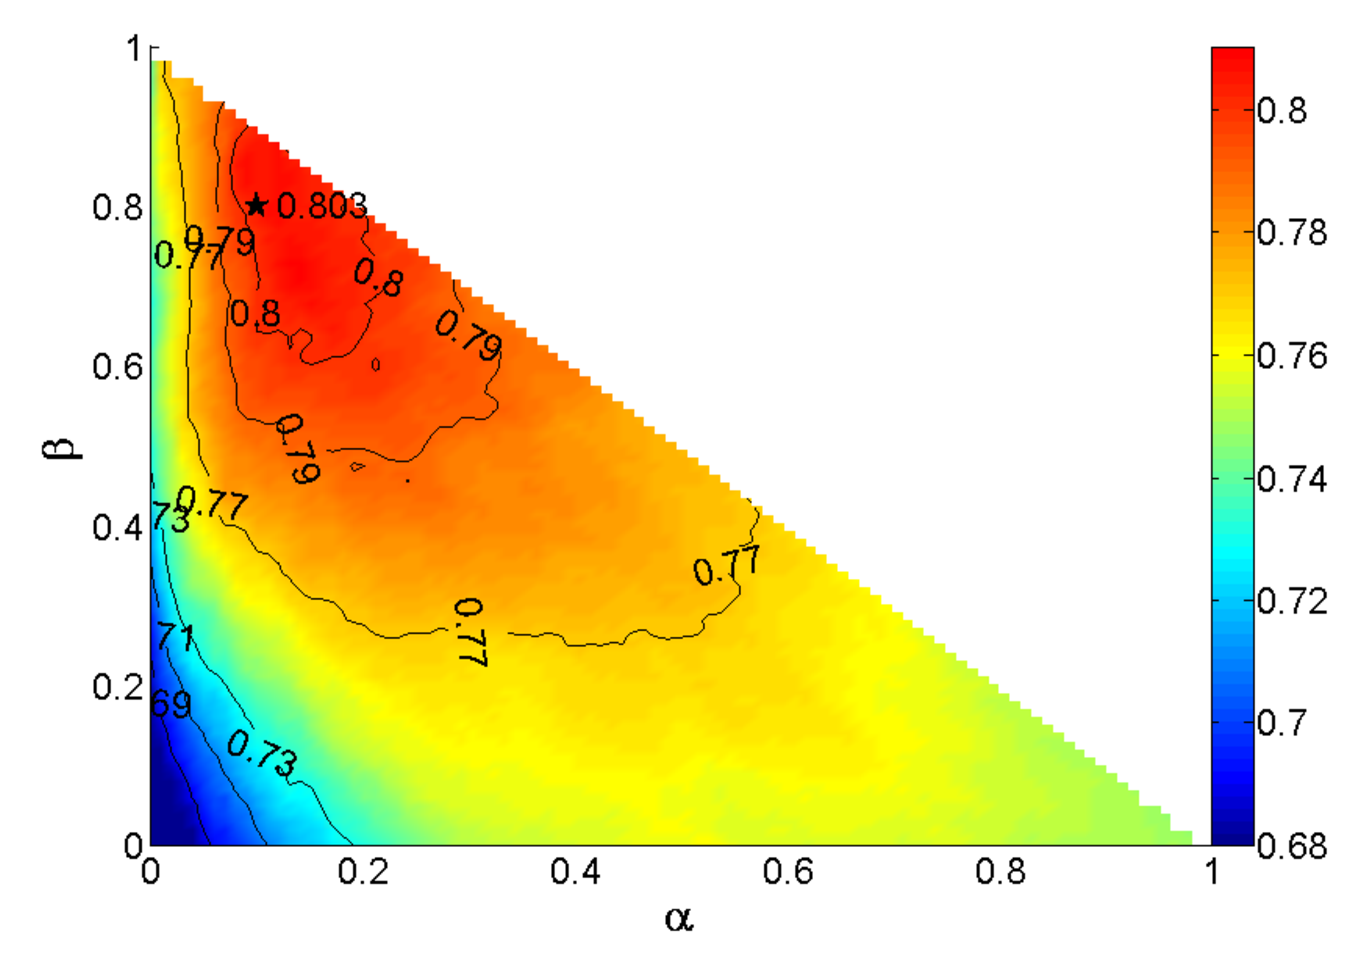
\includegraphics[scale=\graphscaleexpapp]{./exp/AAN-para-recm.eps}}
%\quad\quad
%\hspace{\graphmarginexpapp}
\hfill
\subfigure[{\scriptsize \aminer with \recom}]{\label{exp-aminer-ab-recom}
\includegraphics[scale=\graphscaleexpapp]{./exp/AMiner-para-recm.eps}}
%\quad\quad
%\hspace{\graphmarginexpapp}
\hfill
\subfigure[{\scriptsize \magdata with \recom}]{\label{exp-mag-ab-recom}
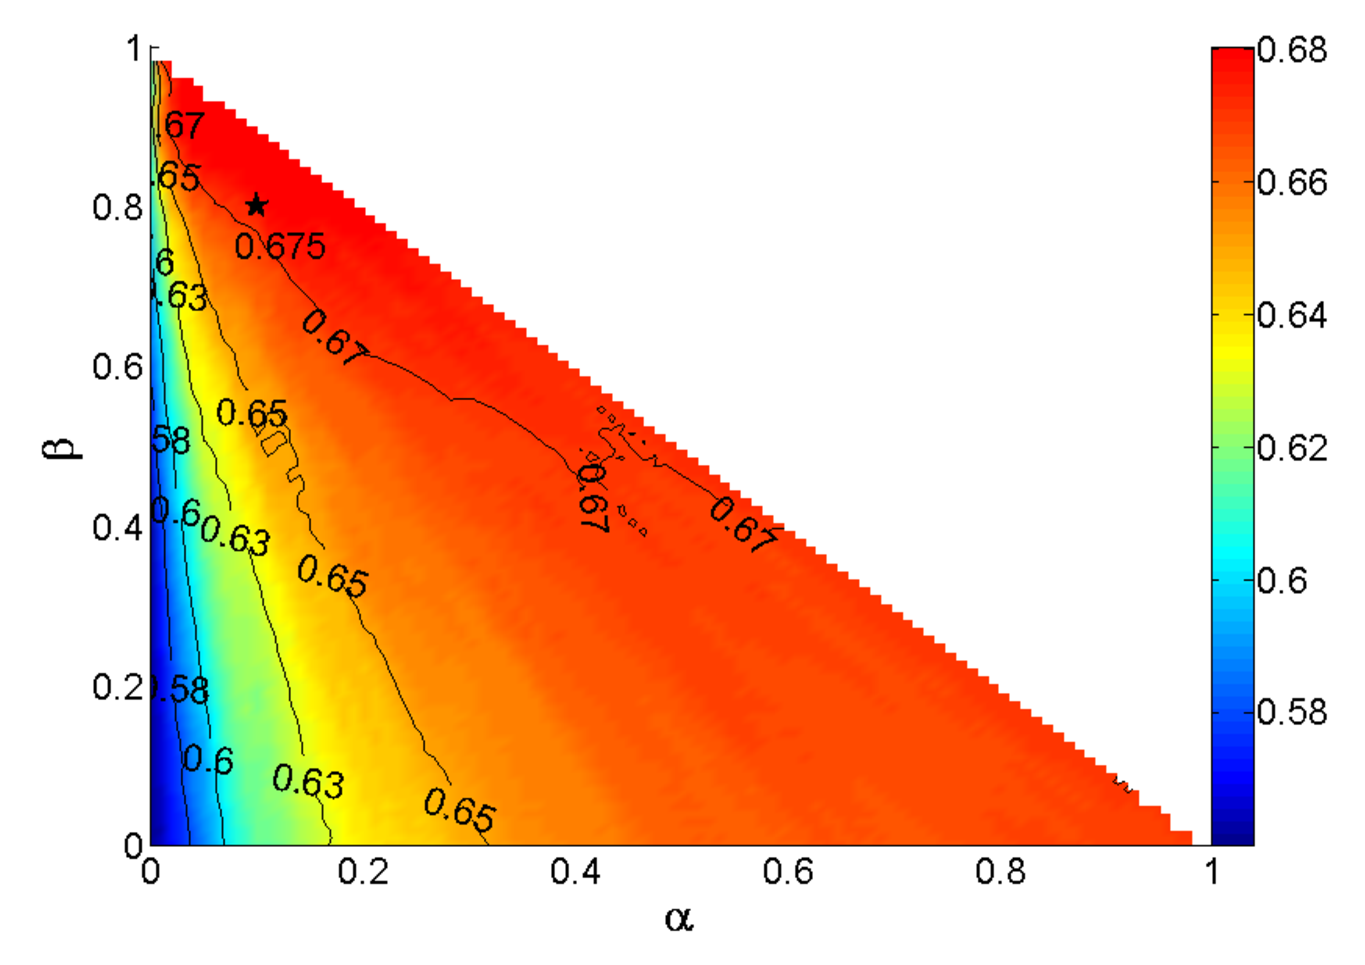
\includegraphics[scale=\graphscaleexpapp]{./exp/MAG-para-recm.eps}}
\\ %%%%%%%%%%%%%%%%%%%%%%%%%%%%%%%%%%%%%%
\vspace{-2ex}
%\hspace{-10ex}
\subfigure[{\scriptsize \aan  with \fcita}]{\label{exp-aan-ab-fcita}
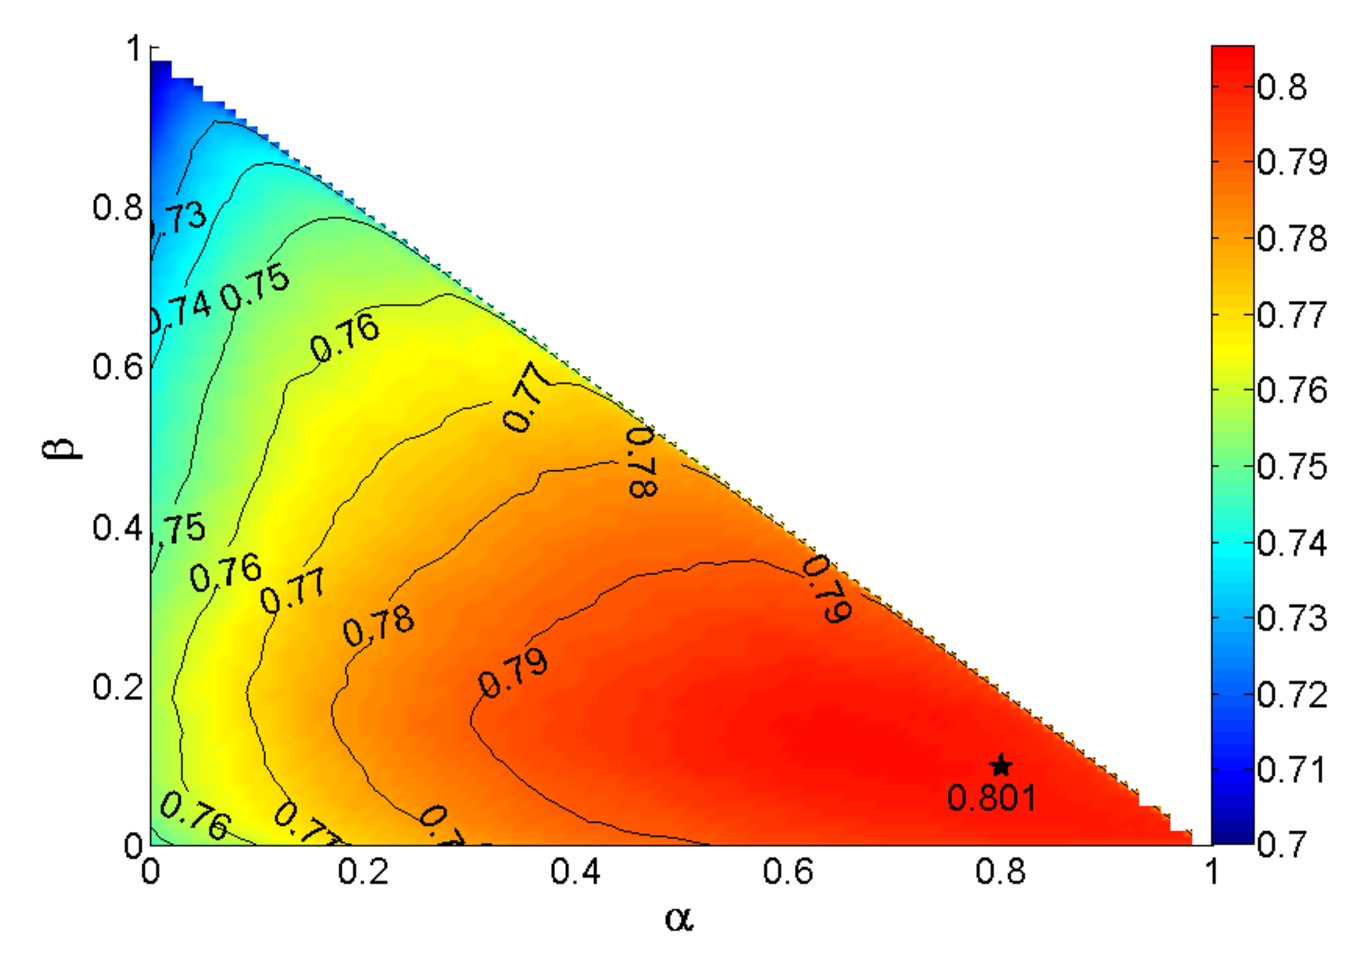
\includegraphics[scale=\graphscaleexpapp]{./exp/AAN-para-fcita.eps}}
%\quad\quad
%\hspace{\graphmarginexpapp}
\hfill
\subfigure[{\scriptsize \aminer with \fcita}]{\label{exp-aminer-ab-fcita}
\includegraphics[scale=\graphscaleexpapp]{./exp/AMiner-para-fcita.eps}}
%\quad\quad
%\hspace{\graphmarginexpapp}
\hfill
\subfigure[{\scriptsize \magdata with \fcita}]{\label{exp-mag-ab-fcita}
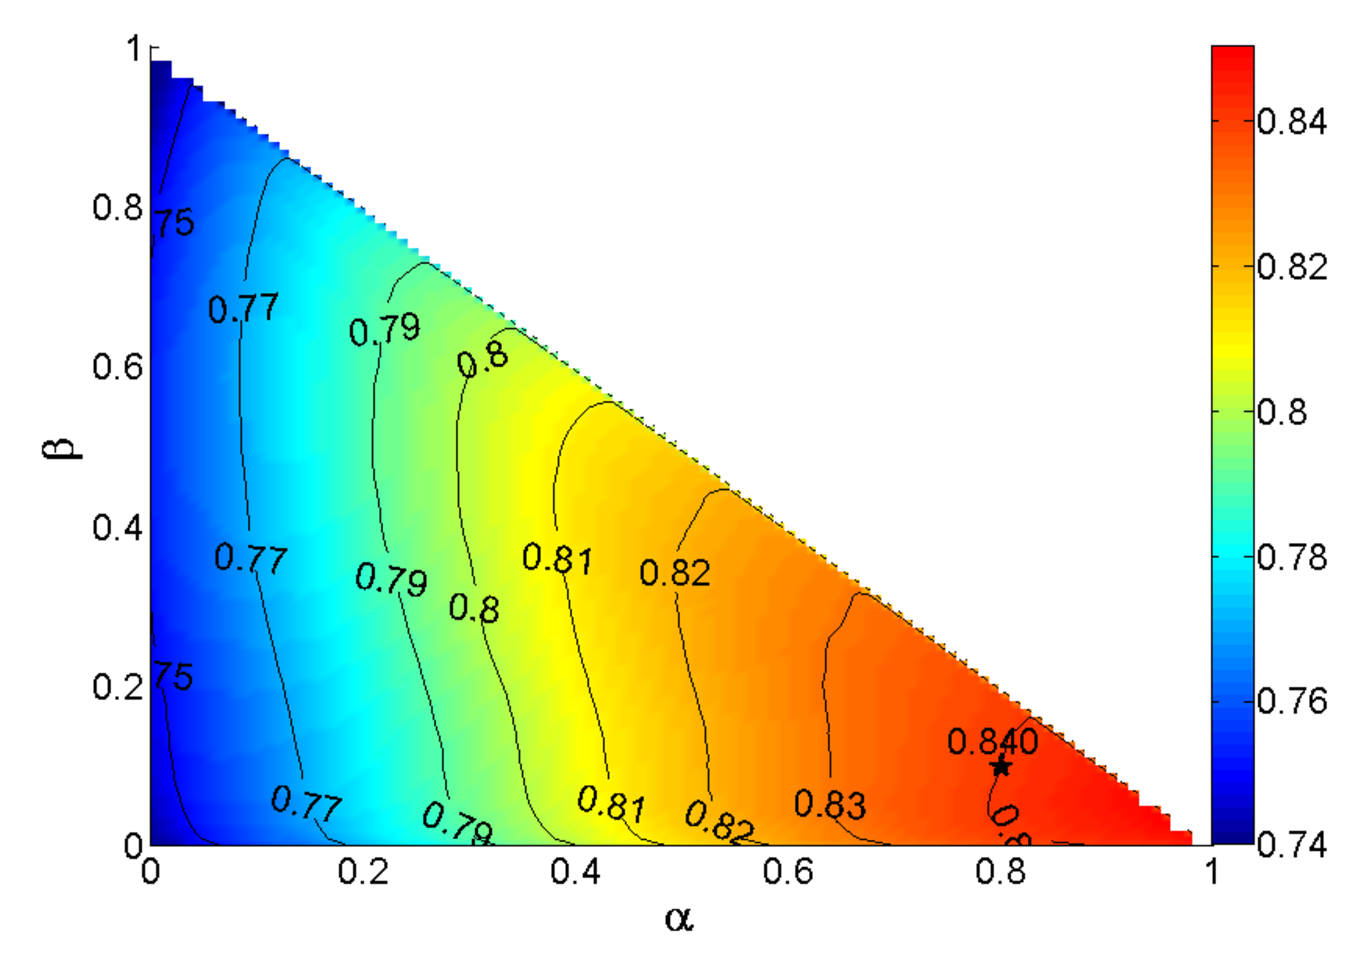
\includegraphics[scale=\graphscaleexpapp]{./exp/MAG-para-fcita.eps}}
\end{center}
\vspace{-2.5ex}
\caption{\small Accuracy tests: varying aggregating parameters $\alpha$ and $\beta$}
\label{exp-ab}
\vspace{-3ex}
\end{figure*}
%%%%%%%%%%%%%%%%%%%%%%%%%%%%%%%%%%%%%%

\stitle{Exp-4: Impacts of parameters}.
%\subsubsection{Exp-4: Impacts of parameters}.
In the last set of tests, we evaluated the impacts of time decaying factor $\sigma$, importance weighting factor $\lambda$, aggregating parameters $\alpha$ and $\beta$, and the TWPageRank. We fixed these parameters as well as $Y_s$ to their default values, used the TWPageRank proposed in this work by default, and tested the \PairAcc with the entire \recom and \fcita (\ie $T_i=+\infty$, $dif=1$).

%We present main results only and more details are available in~\cite{SARank-full}.




\etitle{Exp-4.1}.
%\stitle{Exp-4.1}.
To evaluate the impacts of the time decaying factor $\sigma$, we varied $\sigma$ from -1.6 to -0.4.
%, while fixed $Y_s$ to default values, $T_i=+\infty$, $dif=1$ and $\lambda=0.5$.
The results of \PairAcc are reported in Figs.~\ref{exp-aan-sigma}, \ref{exp-aminer-sigma} and \ref{exp-mag-sigma}.
%with both sets of ground-truth


When varying $\sigma$, the \PairAcc of \ensemblerank is very stable on all datasets using both \recom and \fcita. Indeed, with \recom and \fcita, the \PairAcc only varies (0.42\%, 1.55\%, 0.81\%) and (1.26\%, 0.96\%, 1.16\%) on (\aan, \aminer, \magdata), respectively.
%
%We omitted the detailed results of running time due to space constraint.
The running time varies (11.3\%, 8.6\%) on average only on (\aminer, \magdata), respectively.
%(0.18, 33.6) seconds, \ie

%Both of these show the robustness of \ensemblerank to the time decaying factor $\sigma$.

%As we can see from the figure, our method \ensemblerank is almost stable with the reduction of $\sigma$, since there is only a small fluctuation and the accuracy of our methods is always higher than the best baseline result in all datasets regardless of the change of $\sigma$. This means \ensemblerank is insensitive with $\sigma$.


%%%%%%%%%%%%%%%%%%%%%%%%%%%%%%%%%%%%%%%%%%%%%%%%%%
\begin{table}[tb!]
%\vspace{-2ex}
\begin{center}
\caption{\small Accuracy tests using different components with \recom (rows 2--4) and \fcita (rows 5--7).}
\label{tab-recom}
\begin{small}
\vspace{-.5ex}
\begin{tabular}{|c| c |c | c|}
\hline
{\bf Datasets} & {\bf C}\hspace{5ex}{\bf V}\hspace{5ex}{\bf A} & {\bf CV}\hspace{3ex}{\bf CA}\hspace{3ex}{\bf VA} & {\bf CVA} \\
\hline \hline
% \recom
\aan & 0.752 \ 0.616 \ 0.649 & 0.809 \ 0.764 \ 0.747 & {\bf 0.810} \\
\aminer & 0.735 \  0.581 \  0.640 & 0.784 \ 0.749 \ 0.729 & {\bf 0.785} \\
\magdata & 0.635 \ 0.534 \ 0.553 & 0.697 \ 0.673 \  0.648 & {\bf 0.698} \\ \hline
% \ficta
\aan & 0.785 \ 0.557 \ 0.761 & 0.849 \ 0.866 \ 0.771 & {\bf 0.870} \\
\aminer & 0.713 \  0.603 \  0.725 & 0.843 \ 0.847 \ 0.740 & {\bf 0.856} \\
\magdata & 0.736 \ 0.628 \ 0.718 & 0.848 \ 0.857 \ 0.751 & {\bf 0.874} \\
\hline
\end{tabular}
\end{small}
\end{center}
\vspace{-6ex}
\end{table}
%%%%%%%%%%%%%%%%%%%


\etitle{Exp-4.2}.
%\stitle{Exp-4.2}.
To evaluate the impacts of importance weighting factor $\lambda$, we varied $\lambda$ from 0 to 1.
%while fixed $Y_s$ to default values, $T_i=+\infty$, $dif=1$ and $\sigma=-1.0$.
The results of \PairAcc are reported in Figs.~\ref{exp-aan-lambda}, \ref{exp-aminer-lambda} and \ref{exp-mag-lambda}. Note that parameter $\lambda$ has no impacts on efficiency.
%with both sets of ground-truth

When varying $\lambda$, the \PairAcc of \ensemblerank first increases and then decreases on all datasets with both \fcita and \recom, except on \aminer with \recom.
%\marked{The value of $\lambda$ for \ensemblerank to achieve the best effectiveness is (0.6, 0, 0.2) and (0.6, 0.4, 0.1) on (\aan, \aminer, \magdata) with \recom and \fcita, respectively.}
This result indicates that combining prestige and popularity generally produces more robust results than using either of prestige and popularity.
Indeed, with \recom and \fcita, the \PairAcc of combining prestige and popularity is (10.2\%, 10.7\%, 5.5\%) and (8.0\%, 8.7\%, 9.0\%) higher than using prestige alone, and is (1.2\%, -0.1\%, 1.0\%) and (1.0\%, 1.0\%, 0.3\%) higher than using popularity alone on (\aan, \aminer, \magdata), respectively.


%The selection of $\lambda$ is influenced by ground-truth, such that the best $\lambda$ falls into $[xx,xx]$ and $[yy,yy]$ on \fcita and \recom, respectively. Moreover, equally weighting, \ie $\lambda=0.5$, is a good default setting when no query information is available in advance.
%Indeed, the best obtained \PairAcc using (\fcita, \recom) is only (0.10\%, 0.38\%), (0.04\%, 2.59\%) and (0.06\%, 0.91\%)  higher than the \PairAcc of equally weighting on \aan, \aminer and \magdata, respectively.





\etitle{Exp-4.3}.
To evaluate the impacts of aggregating parameters $\alpha$ and $\beta$, we varied $\alpha$ and $\beta$ at the granularity of 0.01. Again, parameters $\alpha$ and $\beta$ have few impacts on efficiency. The results are reported in Fig.~\ref{exp-ab}, where the parameters selected earlier and their corresponding \PairAcc are marked with $*$.

When varying $\alpha$ and $\beta$, the \PairAcc of \ensemblerank changes gently, as shown in Fig.~\ref{exp-ab}.
The optimal \PairAcc is obtained within a single region, rather than a complex collection of optimal regions.
%
Moreover, the \PairAcc keeps at a high level within a certain ($\alpha$, $\beta$) combination space around the optimal region, as shown in Fig.~\ref{exp-ab}.
%For instance, consider a square of length 0.3, which covers 8.5\% of the parameter combination space. The fraction of parameters such that the \PairAcc is no worse than 1\% of the corresponding \PairAcc with marker $*$ is (73\%, 94\%) on \aan, (96\%, 87\%) on \aminer and (83\%, 95\%) on \magdata, using (\recom, \fcita), respectively.
%
Further, the optimal parameters on the same sets of ground-truth are very similar for (\aan, \aminer and \magdata), indicating that the setting of $\alpha$ and $\beta$ can be easily transferred across different datasets.
To conclude, \ensemblerank is very robust to parameters $\alpha$ and $\beta$, and it is quite flexible for choosing proper values of parameters $\alpha$ and $\beta$.

Moreover, this enables to verify the effectiveness of importance assembling from different components, whose results are reported in Table~IV, in which letters C, V and A stand for citation, venue and author components, respectively.
The ranking based on all components consistently performs the best, using both \recom and \fcita, which justifies the use of importance assembling for ranking scholarly articles.
%which, using \recom and \fcita, improves the \PairAcc over using components (C, V, A, CV, CA, VA) by (5.77\%, 19.4\%, 16.1\%, 0.09\%, 4.59\%, 6.28\%) and (9.54\%, 23.7\%, 5.90\%, 2.50\%, 0.71\%, 4.79\%) on \aan, (6.94\%, 23.7\%, 14.4\%, 0.21\%, 1.56\%, 7.67\%) and (17.68\%, 12.4\%, 9.61\%, 0.33\%, 1.88\%, 6.34\%) on \aminer, and (6.29\%, 16.38\%, 14.45\%, 0.05\%, 2.43\%, 5.02\%) and (11.43\%, 19.2\%, 11.2\%, 1.44\%, 0.77\%, 9.62\%) on \magdata, respectively.


\eat{
\etitle{Exp-4.3}.
%\stitle{Exp-4.3}.
To evaluate the impacts of aggregating parameters $\alpha$ and $\beta$, we varied $\alpha$ and $\beta$ at the granularity of 0.01.
%while fixed $Y_s$ to default values, $T_i=+\infty$, $dif=1$, $\sigma=-1.0$ and $\lambda=0.5$.
Again, parameters $\alpha$ and $\beta$ have few impacts on efficiency. Due to space limitations, we only present the main results and more details are available at~\cite{SARank-full}.

Indeed, \ensemblerank is very robust to parameters $\alpha$ and $\beta$.
(a) When varying $\alpha$ and $\beta$, the \PairAcc of \ensemblerank changes gently. (b) \PairAcc also keeps at a high level within a certain ($\alpha$, $\beta$)  combination space. Finally, (c) the optimal parameters on the same set of ground-truth are very similar for \aan, \aminer and \magdata. That is, it is quite flexible for choosing proper values
of  parameters $\alpha$ and $\beta$.
} %%%%%%%% brief version of Exp-4.3

%%%%%%%%%%%%%%%%%%%%%%%%%%%%%%%%%%%%%%
\begin{figure*}[tb!]
%\vspace{1ex}
\addtolength{\subfigcapskip}{-1ex}
\begin{center}
\subfigure[{\scriptsize \aan with \recom}]{\label{exp-aan-recom-drank}
\includegraphics[scale=0.35]{./exp/AAN_TWPageRank_recom.eps}}
\hfill
%\hspace{\graphmarginexpapp}
\subfigure[{\scriptsize \aminer with \recom}]{\label{exp-aminer-recom-drank}
\includegraphics[scale=0.35]{./exp/AMiner_TWPageRank_recom.eps}}
\hfill
%\hspace{\graphmarginexpapp}
\subfigure[{\scriptsize \magdata with \recom}]{\label{exp-mag-recom-drank}
\includegraphics[scale=0.35]{./exp/MAG_TWPageRank_recom.eps}}
\\%%%%%%%%%%%%%%%%%%%%%%%%%%%%%%%%%%%%%%%%%%%
\vspace{-1.5ex}
\subfigure[{\scriptsize \aan with \fcita}]{\label{exp-aan-fcita-drank}
\includegraphics[scale=0.35]{./exp/AAN_TWPageRank_fcita.eps}}
\hfill
%\hspace{\graphmarginexpapp}
\subfigure[{\scriptsize \aminer with \fcita}]{\label{exp-aminer-fcita-drank}
\includegraphics[scale=0.35]{./exp/AMiner_TWPageRank_fcita.eps}}
\hfill
%\hspace{\graphmarginexpapp}
\subfigure[{\scriptsize \magdata with \fcita}]{\label{exp-mag-fcita-drank}
\includegraphics[scale=0.35]{./exp/MAG_TWPageRank_fcita.eps}}
\end{center}
\vspace{-2.5ex}
\caption{\small Impacts of the TWPageRank on accuracy: varying importance weighting
factor $\lambda$}
\label{exp-drank}
\vspace{-3ex}
\end{figure*}
%%%%%%%%%%%%%%%%%%%%%%%%%%%%%%%%%%

\newcommand{\drank}{\kw{DRank}}


\etitle{Exp-4.4}.
\marked{To evaluate the impacts of the proposed TWPageRank, we compared our approach \ensemblerank with an algorithm alternative (referred to as \drank) the same to \ensemblerank except exploiting exponentially decayed impact weights, \ie $w(u,v)=e^{\sigma(T_u-T_v)}$ in Eq.~(\ref{eq-infl-weights}).
%The two algorithms produce the same popularity while different prestige.
To better understand the impacts, we varied the importance weighting factor $\lambda$ from 0.1 to 1. Note that the ranking results are the same when $\lambda=0$ due to the same popularity computation. The results are reported in Fig.~\ref{exp-drank}, where the numbers represent the improvement of \PairAcc by \ensemblerank over the one by \drank.}

\marked{
When varying $\lambda$, the \PairAcc of \ensemblerank is better than the one of \drank in most cases, which shows the superiority of the TWPageRank than exploiting exponentially decayed weights.
The difference of \PairAcc by the two algorithms is higher with \recom than with \fcita, since the two algorithms are using citation information to predict past and future citations with \fcita.
Moreover, algorithm \ensemblerank is consistently better than \drank when $0.5 \le \lambda \le 0.9$.
%, which, with \recom and \fcita, improves the \PairAcc by (2.88\%, 3.91\%, 3.90\%) and (0.55\%, 0.50\%, 0.22\%) on (\aan, \aminer, \magdata) on average, respectively.
The improvement decreases with the decrease of $\lambda$ as the popularity dominates the ranking with small $\lambda$, and in some cases, \drank outperforms \ensemblerank. %as the prestige and popularity orders of article pairs are more diverse for \drank than \ensemblerank.
Overall, with \recom and \fcita, \ensemblerank improves the \PairAcc over \drank by (1.78\%, 3.07\%, 3.20\%) and (0.29\%, 0.48\%, 0.11\%) on (\aan, \aminer, \magdata) on average, respectively.
}

\marked{
The TWPageRank has little impacts on efficiency, and the running time of the two algorithms only varies (6.34\%, 4.83\%) on (\aminer, \magdata) on average, respectively.}

\eat{
With the increment of $\lambda$, \ensemblerank has more promotion than DRank and the \PairAcc of DRank is better than \ensemblerank with small $\lambda$, possibly due to the addition of popularity will correct the mistaken pairs better on DRank, although \ensemblerank rank more pairs correctly.
In addition, the change of \PairAcc with \recom is higher than the one with \fcita, possibly due to the article pairs in \fcita are of the same years.
Moreover, the \PairAcc of \ensemblerank is better than its counterparts from $\lambda=0.5$ to $\lambda=1$, except on \aminer with \fcita. Recall that in Fig.~\ref{exp-aminer-lambda} using popularity alone gives the best results on \aminer, indicating that the prestige computed by TWPageRank is less accurate on \aminer than on the other two datasets.
%
Indeed, with \recom and \fcita, the \PairAcc of \ensemblerank is (2.20\%, 6.63\%, 5.68\%) and (0.25\%, 0.05\%, 0.05\%) higher than DRank on (\aan, \aminer, \magdata), respectively, when using prestige alone, and is (1.73\%, 2.97\%, 2.92\%) and (0.22\%, -0.08\%, 0.17\%) higher when combining prestige and popularity, respectively, on average.
%
Finally, the TWPageRank has little impacts on efficiency, and the running time of \ensemblerank and its counterparts only changes (6.34\%, 4.83\%) on (\aminer, \magdata) on average, respectively.
}

\stitle{Summary}.
From these tests we find the followings.


\sstab(1) Our model \ensemblerank is effective for ranking scholarly articles, which is consistently better than competitive methods in all tests. With \recom and \fcita, \ensemblerank improves \PairAcc over (\pagerank, \futurerank, \hhgrank) by
(13.5\%, 6.8\%, 4.8\%) and (12.0\%, 3.0\%, 3.2\%) on \aan,
(12.7\%, 5.0\%, 4.9\%) and (14.0\%, 6.5\%, 4.6\%) on \aminer, and
(6.5\%, 2.5\%, 2.2\%) and (13.4\%, 6.0\%, 2.4\%) on \magdata, on average, respectively.
%, and it has a great advantage in evaluating the importance in a long term. Furthermore, it is more accurate evaluating articles which have just published and is in lack of citations, since it uses both venue network and author information besides of citation network. Indeed, it improves the accuracy by $(7.9\%, 3.2\%, 2.3\%)$ and $(14.4\%, 5.0\%, 3.8\%)$ over \pagerank, \futurerank and \hhgrank on average of three datasets with recommendation based ground truth and future citation ground truth, respectively.


\sstab(2) Our batch algorithm \batensemble and incremental algorithm \incensemble are also efficient.
%
Our incremental algorithm \incensemble is on average (1.7, 3.1, 2.8, 117) and (2.0, 3.0, 4.4, 245) times faster than (\batensemble, \powensemble, \futurerank, \hhgrank)  on the large \aminer and \magdata, respectively.

%The batch algorithm \batensemble is on average (1.3, 2.5, 348) times faster than (\powensemble, \futurerank, \hhgrank)  on the largest \magdata, respectively.

%\noindent (3) Our incremental algorithms are much faster than their batch counterparts in practice, even their time complexity is very close. Indeed, algorithms \inctwprdag, \inctwprscc and \incensemble further improve the efficiency of (\twprdag, \twprscc, \batensemble) by (23\%, 38\%, 22\%) on average, respectively.


\sstab(3) Our ranking model \ensemblerank introduces the time decaying factor $\sigma$, importance weighting factor $\lambda$ and aggregating parameters $\alpha$ and $\beta$ for the sake of practicability and flexibility in real-life applications, and, from our tests, \ensemblerank is very robust to these parameters. Moreover, the proposed TWPageRank is generally more effective than directly using exponentially decayed impact weights.




%\stitle{Related work}. We summarize related work as follows.
%
%Scholarly article ranking

Scholarly article ranking has shifted from citation count analysis~\cite{Garfield471,Hirsch15112005} to graph analysis~\cite{ChenXMR07,Zhou07-CoRank,Jiang12-MRank,Liang16AAAI,Li08TSRanking,Wang13AAAI,WalkerXKM07,sayyadi09,
Wang16TIST,Ng11KDD}.
Based on the information used, these methods are divided into four categories: (a) using the citation information only~\cite{Garfield471,Hirsch15112005,ChenXMR07,Ng11KDD}, (b) using the citation and temporal information~\cite{Li08TSRanking,WalkerXKM07}, (c) using the citation information and other heterogeneous information, \eg authors and venues of articles~\cite{Zhou07-CoRank,Jiang12-MRank,Liang16AAAI}, and (d) combining the citation, temporal and other heterogeneous information~\cite{sayyadi09,Wang16TIST,Wang13AAAI}.
Our work belongs to the last category aiming at fully employing information available for scholarly article ranking.


%\stitle{PageRank\&weighted PageRank algorithms}.

%PageRank \cite{Brin98:PageRank} and its extensions have been extensively used for citation analyses \cite{Waltman2014}. While PageRank equally propagates scores along outlinks, Weighted PageRank \cite{Xing04:WPR} extends PageRank by distributing scores based on the popularity of pages. Different from previous work, the Time-Weighted PageRank proposed in this work discriminately propagates scores in terms of citation statistics.

PageRank \cite{Brin98:PageRank} and its extensions have been extensively used for citation analyses \cite{Waltman2014}. While PageRank equally propagates scores along outlinks, Weighted PageRank extends PageRank by distributing scores based on certain criteria such as popularity of pages~\cite{Xing04:WPR} or authority of authors~\cite{Ding11}. Different from previous work, the Time-Weighted PageRank proposed in this work discriminately propagates scores in terms of citation statistics.






%\stitle{Dynamic algorithms}.

Dynamic algorithms have proven useful for various tasks by avoiding computing from scratch~\cite{RamalingamR93}.
% and only recomputing those affected by updates
%Dynamic algorithms have proven useful for graph analysis tasks, \eg incremental graph pattern matching~\cite{FanWW13} and  incremental simrank computation~\cite{YuLZ14}.
To our knowledge, little concern has been paid to dynamic scholarly article ranking except that~\cite{GhoshKHLL11} uses PageRank in dynamic citation networks. However, its solution is based on a strong and impractical assumption that there are no citations between articles in the same years.
Further, although there exist several studies on incremental PageRank computation~\cite{DesikanPSK05,AbiteboulPC03,WuR09} and on incremental PageRank approximation \cite{BahmaniCG10,BahmaniKMU12}, they are not designed for scholarly article ranking.
%
Different from previous work, we study scholarly article ranking in a dynamic environment in terms of
the citation characteristics of scholarly articles, which has never been exploited before.

%Our approach only makes the assumption that there are no mutual references within the citation network, which, we admit, violates xx\% of total citations on \magdata, and is significantly different (yy\% on \magdata) from~\cite{GhoshKHLL11}.  - move to Section 3

Ensemble methods use multiple learners to obtain better performance than could be obtained from a constituent learner alone~\cite{zhihua-book}.
%In this work, we leverage ensembles to produce better and robust results for scholarly article ranking~\cite{zhihua-book,wsdmcup,DuanAMHH16}.
In this work, we leverage  importance assembling  to produce better and robust results for scholarly article ranking~\cite{zhihua-book,wsdmcup,DuanAMHH16}.

%\vspace{-0.5ex}
\section{Conclusions}
\label{sec-conclude}
%\vspace{-1ex}

We have proposed \pCFDs and \pCINDs, which further extend \CFDs and \CINDs,
respectively,  by allowing patterns on data values to be expressed in
terms of $\ne, <, \le, >$ and
$\ge$ predicates. We have shown that \pCFDs and \pCINDs
are more powerful than \CFDs and \CINDs for detecting errors
in real-life data. In addition, the
satisfiability and implication problems for \pCFDs and \pCINDs have
the same complexity bounds as their counterparts for \CFDs and
\CINDs, respectively. We have also provided automated methods to
generate \SQL queries for detecting errors based on \pCFDs and
\pCINDs. These provide commercial \rdms with an immediate capability to
capture errors commonly found in real-world data.


One topic for future work is to develop a dependency language that
is capable of expressing various extensions of \CFDs (\eg \pCFDs,
e\CFDs~\cite{icde08} and {{\sc cfd$^c$}{\small s}~\cite{ChenFM09}),
without increasing the complexity of static analyses. Second, we are
developing effective algorithms for discovering \pCFDs and \pCINDs,
along the same lines as \cite{CM08,divesh08,icde09}. Third, we plan
to extend the methods of~\cite{sigmod05,repair} to repair data based
on \pCFDs and \pCINDs, instead of using \CFDs~\cite{repair},
traditional \FDs and \INDs~\cite{sigmod05}, denial
constraints~\cite{BertossiBFL08,ChomickiM05}, and aggregate
constraints~\cite{FlescaFP05}.


\vspace{-2ex}
\section*{Acknowledgments}
Ma is supported in part by  973 program 2014CB340300 and NSFC 61322207.
Fan is supported in part by
NSFC  61133002,  973 Program 2014CB340302,
Shenzhen Peacock Program 1105100030834361, Guangdong Innovative Research Team
Program 2011D005, EPSRC EP/J015377/1 and EP/M025268/1,
and a Google Faculty Research Award.




% trigger a \newpage just before the given reference
% number - used to balance the columns on the last page
% adjust value as needed - may need to be readjusted if
% the document is modified later
%\IEEEtriggeratref{8}
% The "triggered" command can be changed if desired:
%\IEEEtriggercmd{\enlargethispage{-5in}}

% references section

% can use a bibliography generated by BibTeX as a .bbl file
% BibTeX documentation can be easily obtained at:
% http://www.ctan.org/tex-archive/biblio/bibtex/contrib/doc/
% The IEEEtran BibTeX style support page is at:
% http://www.michaelshell.org/tex/ieeetran/bibtex/
%\bibliographystyle{IEEEtran}
% argument is your BibTeX string definitions and bibliography database(s)
%\bibliography{IEEEabrv,../bib/paper}
%
% <OR> manually copy in the resultant .bbl file
% set second argument of \begin to the number of references
% (used to reserve space for the reference number labels box)
%%%%%%%%%%%%%%%%%%%%%%%%%%%%%%%%%%%%%%%%%%%
%\enlargethispage{-5in}
%\vspace{-2ex}
%\renewcommand{\baselinestretch}{0.92}
%\setlength{\baselineskip}{6pt}
%\balance
%\begin{footnotesize}
\bibliographystyle{abbrv}
\bibliography{paper}
%\end{footnotesize}

\vspace{-6ex}
\begin{IEEEbiography}{Shuai Ma} is a professor at the School of Computer Science and Engineering, Beihang University.
He obtained his PhD degrees from University of Edinburgh in 2010, and from
Peking University in 2004, respectively.
He was a postdoctoral research fellow in the database group,
University of Edinburgh, a summer intern at Bell labs, Murray Hill, USA, in the summer of 2008, and a visiting researcher of MRSA in 2012.
He is a recipient of the Best Paper Award for VLDB 2010  and the Best Challenge Paper Award for WISE 2013. His current research interests include database theory and systems, social data analysis and data intensive computing.
\end{IEEEbiography}
\vspace{-6ex}
\begin{IEEEbiography}{Liang Duan} is a PhD student in the School of Computer Science and Engineering, Beihang University, co-supervised by Prof. Jinpeng Huai and Prof. Shuai Ma. He received his MS degree in computer software and theory from Yunnan University in 2014, and BS degree in computer science and technology from Beihang University in 2009. His current research interests include databases and social data analysis.
\end{IEEEbiography}
\vspace{-6ex}
\begin{IEEEbiography}{Wenfei Fan} is Professor (Chair) of Web Data Management in
the School of Informatics, University of Edinburgh, UK.
He is a Fellow of ACM, a Fellow of the Royal Society of Edinburgh, UK,  a
National Professor of the Thousand-Talent Program and a
Yangtze River Scholar, China.  He received his PhD degree from the
University of Pennsylvania. He is a recipient of the Runner-up for Best Paper Award of ICDE 2014, the Alberto O. Mendelzon
Test-of-Time Award of ACM PODS 2010, the Best Paper Award
for VLDB 2010, the Roger Needham Award in 2008 (UK), the
Best Paper Award for ICDE 2007, the Best Paper of the Year
Award for Computer Networks in 2002, and the Career Award
in 2001 (USA). His current research interests include database
theory and systems.
\end{IEEEbiography}
\vspace{-6ex}
\begin{IEEEbiography}{Chunming Hu} is an associate professor at the School of Computer Science and Engineering, Beihang University.  He received his PhD degree from Beihang University in 2006. His current research interests include distributed systems, system virtualization, large scale data management and processing systems.
\end{IEEEbiography}
\vspace{-6ex}
\begin{IEEEbiography}{Wenguang Chen} is an associate professor at the Department of Computer Science, Peking University. He obtained his PhD degree from Peking University in 2009.  He was a visiting scholar at University of Alberta from 2011 to 2012 and at University of Hawaii at Manoa in from 2012 to 2013. His current research interests include data management, data quality and intelligent HCI.
\end{IEEEbiography}
\vfill

%\appendices
%\newpage
\section*{{\Large \sf APPENDIX}}
\label{sec-appendix}


\subsection{SQL queries for CFD$^p$s}

 We first present the generation of
detection queries for \pCFDs, which is an extension of the
\SQL techniques for \CFDs and \eCFDs discussed in~\cite{CFDs} and ~\cite{icde08}, respectively.

%%%%%%%%% DL 2014-08-09
The queries for the violations of $\SCFD^i$ are given as follows, which capitalize on the data table \Enc{L}, \Enc{R} and \Enc{\ne} that encode \pCFDs in $\SCFD^i$.

\begin{footnotesize}\mat{0ex}{
$Q^C$ \= \bd{select} \=  $R_i.*$ \bd{from} $R_i$, \Enc{L} $L$, \Enc{R} $R$, \Enc{\ne} $N$ \\
\>  \bd{where} $L.\at{cid}=R.\at{cid}$ \bd{and} $R_i.X\asymp L$ \bd{and} $R_i.X\asymp N$ \\
\> \> \bd{and not} ($R_i.Y\asymp R$ \bd{and} $R_i.Y\asymp N$)}
\end{footnotesize}

\begin{footnotesize}\mat{0ex}{
$Q^V$ \= \bd{select} \= \bd{distinct } \= $X$ \bd{from ( select} $L.\at{cid}$, \\
\>  (\bd{case when} $L.X_j$ \bd{is null then null} \bd{else} $R_i.X_j$ \bd{end}) \bd{as} $X_j$\bd{...} \\
\>  (\bd{case when} $R.Y_k$ \bd{is null then null} \bd{else} $R_i.Y_k$ \bd{end}) \bd{as} $Y_k$\bd{...}\\
\>\> \bd{from} $R_i$, \Enc{L} $L$, \Enc{R} $R$, \Enc{\ne} $N$ \\
\>\> \bd{where} $L.\at{cid}=R.\at{cid}$ \bd{and} $R_i.X\asymp L$ \bd{and} $R_i.X\asymp N$ \\
\>\>\> \bd{and} ($R.Y_1='\_'$ \bd{or} $R.Y_2='\_'$ \bd{or ...} )) $M$\\
\>\>\> \bd{group by} $X$, \at{cid} \bd{having count} (\bd{distinct} $Y$)$>1$}
\end{footnotesize}

\noindent Here (1) $X$ and $Y$ are the sets of attributes in \LHS and \RHS of $\SCFD^i$ respectively; (2) $R_i.X\asymp L$ is shorthand for the conjunction of

\begin{footnotesize}\mat{0ex}{
$L.A_k$ \= \bd{is null or} $R_i.A_k$ = $L.A_k$ \bd{or} ($L.A_k$ = '\_'\\
\> \bd{and} ($L.A_{k_{>}}$ \bd{is null or} $R_i.A_k$ $>$ $L.A_{k_{>}}$)\\
\>  \bd{and} ($L.A_{k_{\ge}}$ \bd{is null or} $R_i.A_k$ $\ge$ $L.A_{k_{\ge}}$)\\
\> \bd{and} ($L.A_{k_{<}}$ \bd{is null or} $R_i.A_k$ $<$ $L.A_{k_{<}}$)\\
\> \bd{and} ($L.A_{k_{\le}}$ \bd{is null or} $R_i.A_k$ $\le$ $L.A_{k_{\le}}$))
}
\end{footnotesize}

\noindent for each $A_{k} \in X$; (3) $R_i.Y\asymp R$ is defined similarly for attributes in $Y$; (4) $R_i.X\asymp N$ is the conjunction

\begin{footnotesize}\mat{1ex}{
\bd{not exists}
(\=\bd{select} $*$ \bd{from} $N$ \\
\>\bd{where} \= $L.\at{cid}$ = $N.\at{cid}$ \bd{and} $N.\at{pos}$ = `\LHS' \bd{and}\\
\>\>  $N.\at{att}$ = `$A_k$' \bd{and}
 $R_i.A_k$ = $N.\at{val}$);
}
\end{footnotesize}

\noindent for $A_{k} \in X$; (5) $R_i.Y\asymp N$ is defined similarly, but with $N.\at{pos}='\RHS'$.

Intuitively, detecting violations of \pCFDs in $\SCFD^i$ is a two-step process. Firstly, query $Q^{C}$ detects single-tuple violations, that is the tuples $t$ in $I_{i}$ that match the \LHS patterns of some \pCFDs in $\SCFD^i$, but $t$ does not match the corresponding \RHS patterns of these \pCFDs. Secondly, query $Q^{V}$ finds multi-tuple violations, that is, tuples $t$ in $I_{i}$ for which there exists a tuple $t'$ in $I_{i}$ such that $t[X]=t'[X] \asymp L$, but $t[Y] \neq t'[Y]$. Query $Q^{V}$ uses the \bd{group by} clause to group tuples with the same value on $X$ and it counts the number of distinct $Y$. If there is more than one instantiation, then there is a violation.

\begin{example}\label{exa-cfd-query} Using the coding of Fig.~\ref{fig-pcfd-encoding}, two SQL queries for checking \pCFDs $\varphi_2$, $\varphi_3$ and $\varphi_4$ of Fig.~\ref{fig-pcfd} are given as follows:

\begin{footnotesize}\mat{0ex}{
$Q^C$ \= \bd{select} \=  $R_1.*$ \= \bd{from}  \at{item} $R_1$, \Enc{L} $L$, \Enc{R} $R$, \Enc{\ne} $N$\\
 \> \bd{where} $L.\at{cid}=R.\at{cid}$ \bd{and} ($L.\at{sale}$ \bd{is null or} $R_1.\at{sale}=L.\at{sale}$\\
 \> \> \bd{or} $L.\at{sale}='\_'$) \bd{and not exists} ( \bd{select * from} $N$\\
 \> \> \> \bd{where} $N.\at{cid}=L.\at{cid}$ \bd{and} $N.\at{pos}='\LHS'$ \bd{and} \\
 \> \> \> $N.\at{att}='sale'$ \bd{and} $R_{1}.\at{sale}=N.\at{val}$) \bd{and} \\
 \>\> ($L.\at{price}$ \bd{is null or} $R_1.\at{price}=L.\at{price}$ \bd{or} ($L.\at{price}='\_'$  \\
 \> \> \bd{and} ($L.\at{price_>}$ \bd{is null or} $R_1.\at{price}>L.\at{price_>}$)  \\
 \> \> \bd{and} ($L.\at{price_\leq}$ \bd{is null or} $R_1.\at{price}\leq L.\at{price_\leq}$))) \\
 \> \> \bd{and not exists} ( \bd{select * from} $N$ \\
 \>\>\> \bd{where} $N.\at{cid}=L.\at{cid}$ \bd{and} $N.\at{pos}='\LHS'$ \bd{and} \\
 \> \> \> $N.\at{att}='price'$ \bd{and} $R_{1}.\at{price}=N.\at{val}$) \bd{and not}\\

 \> \> (($R.\at{shipping}$ \bd{is null or} $R_1.\at{shipping}=R.\at{shipping}$ \bd{or}\\
 \> \> $R.\at{shipping}='\_'$\bd{) and not exists} ( \bd{select * from} $N$  \\
 \> \> \> \bd{where} $N.\at{cid}=R.\at{cid}$ \bd{and} $N.\at{pos}='\RHS'$ \bd{and} \\
 \> \> \> $N.\at{att}='shipping'$ \bd{and} $R_{1}.\at{shipping}=N.\at{val}$) \bd{and} \\

 \> \> ($R.\at{price}$ \bd{is null or} $R_1.\at{price}=R.\at{price}$ \bd{or} ($R.\at{price}='\_'$  \\
 \> \> \bd{and} ($R.\at{price_\geq}$ \bd{is null or} $R_1.\at{price}\geq R.\at{price_\geq}$)   \\
 \> \> \bd{and} ($R.\at{price_<}$ \bd{is null or} $R_1.\at{price}<R.\at{price_<}$)))  \\
 \> \> \bd{and not exists} (\bd{select * from} $N$  \\
 \> \> \> \bd{where} $N.\at{cid}=R.\at{cid}$ \bd{and} $N.\at{pos}='\RHS'$ \bd{and} \\
 \> \> \> $N.\at{att}='price'$ \bd{and} $R_{1}.\at{price}=N.\at{val}$) ) }
\end{footnotesize}

\begin{footnotesize}\mat{0ex}{
$Q^V$\= \bd{select} \= \bd{distinct} \= \at{sale_x}, \at{price_x} \bd{from} ( \bd{select} $L.\at{cid}$, \\
 \> (\bd{case when} $L.\at{sale}$ \bd{is null then null else} $R_1.\at{sale}$ \bd{end}) \bd{as} \at{sale_x},\\
 \> (\bd{case when} $L.\at{price}$ \bd{is null then null else} $R_1.\at{price}$ \bd{end}) \bd{as} \at{price_x},\\
 \> (\bd{case when} $R.\at{shipping}$ \bd{is null then null else} $R_1.\at{shipping}$ \bd{end})\\
 \> \bd{as} \at{shipping_y},  \\
 \> (\bd{case when} $R.\at{price}$ \bd{is null then null else} $R_1.\at{price}$ \bd{end}) \bd{as} \at{price_y}  \\
 \> \bd{from} \at{item} $R_1$, \Enc{L} $L$, \Enc{R} $R$, \Enc{\ne} $N$ \\

 \> \bd{where} $L.\at{cid}=R.\at{cid}$ \bd{and} ($L.\at{sale}$ \bd{is null or} $R_1.\at{sale}=L.\at{sale}$\\
 \> \> \bd{or} $L.\at{sale}='\_'$) \bd{and not exists} ( \bd{select * from} $N$\\
 \> \> \> \bd{where} $N.\at{cid}=L.\at{cid}$ \bd{and} $N.\at{pos}='\LHS'$ \bd{and} \\
 \> \> \> $N.\at{att}='sale'$ \bd{and} $R_{1}.\at{sale}=N.\at{val}$) \bd{and} \\
 \>\> ($L.\at{price}$ \bd{is null or} $R_1.\at{price}=L.\at{price}$ \bd{or} ($L.\at{price}='\_'$  \\
 \> \> \bd{and} ($L.\at{price_>}$ \bd{is null or} $R_1.\at{price}>L.\at{price_>}$)  \\
 \> \> \bd{and} ($L.\at{price_\leq}$ \bd{is null or} $R_1.\at{price}\leq L.\at{price_\leq}$))) \\
 \> \> \bd{and not exists} (\bd{select * from} $N$ \\
 \>\>\> \bd{where} $N.\at{cid}=L.\at{cid}$ \bd{and} $N.\at{pos}='\LHS'$ \bd{and} \\
 \> \> \> $N.\at{att}='price'$ \bd{and} $R_{1}.\at{price}=N.\at{val}$) \bd{and}\\

 \> \> ($R.\at{shipping}='\_'$\bd{or} $R.\at{price}='\_'$))  $M$ \\
 \> \> \bd{group by} $\at{sale_x}, \at{price_x}$, \at{cid} \\
 \> \> \> \bd{having count} (\bd{distinct} $\at{shipping_y}, \at{price_y}$)$>1$ }
\end{footnotesize}

\end{example}


%%%%%%%%% DL


%%%%%%%%%%%%%%%%%%%%%%%%%%%%%%%%%%%%%%%%%%%%%%%%%%%%%%%%%%%%%%%%%%%%%%%%%%%%%%%%%%%%%%%%%
\eat{%%%%%%%%%%%%%%%%%
%Proposition 1
\noindent\bd{Proposition}~\ref{thm-sat-pcfd-fin}.~The satisfiability
problem for \pCFDs is \NP-complete. \eop

\begin{proof}
The lower bound follows from the \NP-hardness of their \CFDs
counterparts~\cite{CFDs}, since \CFDs are a special case of \pCFDs.

We next show that the problem is in \NP by presenting an \NP
algorithm that, given a set $\Sigma$ of \pCFDs defined on a
relational schema $R$, determines whether $\Sigma$ is satisfiable.
The satisfiability problem has the following small model property:
If there exists a nonempty instance $I$ of $R$ such that
$I\models\Sigma$, then for any tuple $t\in I$, $I_t$ =$\{t\}$ is an
instance of $R$ and $I_t\models\Sigma$. Thus it suffices to consider
single-tuple instances $I$ = $\{t\}$ for deciding whether $\Sigma$
is satisfiable.

Assume \kwlog that the attributes $\attrset(R)$ = $\{A_1,\dots,
A_m\}$ and the total number of pattern tuples of all pattern
tableaux $T_p$ in $\Sigma$ is $h$. For each $i\in [1, m]$, define
the active domain of $A_i$ to be a set $\adom(A_i)$ = $C_0\cup C_1$,
where (1) set $C_0$ consists of all constants in $T_p[A_i]$ of all
pattern tableaux $T_p$ in $\Sigma$ and let $C_0$ = $\{a_1\}$, where
$a_1\in\dom(A_i)$, if $C_0$ is empty, and (2) set $C_1$ contains the
following set of constants for those attributes whose domains have
total orders: \vspace{-0.5ex}\bi
\item Arrange all constants in $C_0$ in the increasing order, and
assume that the resulting $C_0$ = $\{a_1, \ldots, a_k\}$ ($k\ge 1$);
\item Add a constant $b_{01}\in\dom(A_i)$ to $C_1$ such that $b_{01} < a_1$ if there
exists one; And add another constant $b_{02}\in\dom(A_i)$ to $C_1$
such that $b_{01} < a_1$ and $b_{01}\ne b_{02}$ if there exists one;
\item Similarly, for each $j\in[1, k - 1]$, add a constant $b_{j1}\in\dom(A_i)$ to $C_1$
such that $b_{j1} > a_j$ and $ b_{j1} < a_{j+1}$ if there exists
one; And add another constant $b_{j2}\in\dom(A_i)$ to $C_1$ such
that $b_{j2} > a_j$, $ b_{j2} < a_{j+1}$ and $b_{j1}\ne b_{j2}$ if
there exists one;
\item Add a constant $b_{k1}\in\dom(A_i)$ to $C_1$ such that $b_{k1} > a_k$ if there exists one;
And add another constant $b_{k2}\in\dom(A_i)$ to $C_1$ such that
$b_{k2} > a_k$ if there exists one. \ei\vspace{-1.5ex}

\noindent Moveover, the number of elements in $\adom(A_i)$ is at
most $O(3*h + 2)$. Then one can easily verify that $\Sigma$ is
satisfiable iff there exists a mapping $\rho$ from $t[A_i]$ to
$\adom(A_i)$ ($i\in [1, m]$) such that $I$ = $\{(\rho(t[A_1]),
\ldots, \rho(t[A_m]))\}$ and $I \models \Sigma$.


Based on these, we give an \NP algorithm as follows: (1) Guess an
instance, which contains a single tuple $t$ of $R$ such that
$t[A_i]\in\adom{A_i}$ for each $i \in [1, m]$. (2) Check whether $I
\models \Sigma$. If so the algorithm returns ``yes'', and otherwise
it repeats steps (1) and (2). Obviously step (2) can be done in
\PTIME in the size of $\Sigma$. Hence the algorithm is in \NP, and
so is the problem. \eop
\end{proof}

%Theorem 2
\vspace{2ex} \noindent\bd{Theorem}~\ref{thm-sat-pcfd-infin}.~In the
absence of finite domain attributes, the satisfiability problem for
\pCFDs remains \NP-complete. \eop

\begin{proof}
The problem is in \NP following from
Proposition~\ref{thm-sat-pcfd-fin}. We next show that the problem is
\NP-hard by reduction from the \kSAT\ problem, which is \NP-complete
(cf.~\cite{GaJo79}). Consider an instance $\phi = C_1 \land \cdots
\land C_n$ of \kSAT, where all the variables in $\phi$ are $x_1,
\ldots, x_m$, $C_j$ is of the form $y_{j_1} \lor y_{j_2} \lor
y_{j_3}$, and moreover, for $i\in[1,3]$, $y_{j_i}$ is either
$x_{p_{ji}}$ or $\overline{x_{p_{ji}}}$ for $p_{ji} \in [1, m]$.
Given $\phi$, we construct a relation schema $R$ and a set $\Sigma$
of \pCFDs defined on $R$ such that $\phi$ is satisfiable iff
$\Sigma$ is satisfiable.

\noindent (1) Define relation $R$$(X_1, \ldots, X_m, C_1, \ldots,
C_n, Z)$, where all attributes share an infinite domain $\dom$ and
constant $a\in\dom$. Intuitively, for each $R$ tuple $t$, $t[X_1,$ $
\ldots,$ $X_m]$ specifies a truth assignment $\xi$ for variables
$x_1, \ldots, x_m$ of $\phi$, and $t[C_i]$ and $t[Z]$ are the truth
values of clause $C_i$ and sentence $\phi$ \wrt $\xi$ respectively.

\noindent (2) Let the set $\Sigma$ of \pCFDs be
$\Sigma_0\cup\Sigma_1\cup\ldots\cup\Sigma_n\cup\Sigma_{n+1}$.

\vspace{-1.5ex}\bi
\item $\Sigma_0$ contains $n + 1$ \pCFDs. Intuitively, $\Sigma_0$
encodes the relationships between the truth values of clauses $C_1,
\ldots, C_n$ and the truth value of sentence $\phi$.

For each clause $C_i$ ($i\in[1, n]$), we define \pCFD $\varphi_i$ =
$(C_1,\ldots, C_n\ra Z, T_{pi})$ such that $T_{pi} = \{t_{pi}\}$ and
$t_{pi}[C_i,Z]$ = $(\ne a \pa \ne a)$ and $t_{pi}[C_j]$ = `\_'
($j\ne i, j\in[1, n]$). Moreover, \pCFD $\varphi_{0}$ =
$(C_1,\ldots, C_n\ra Z, T_{p0})$, where $T_{p0}$ = $\{(= a, \ldots,
=a \pa = a)\}$. Intuitively, we use $\ne a$ and $= a$ to represent
{\em false} and {\em true} for the truth values of the clauses and
the sentence.

\item For $i\in[1, n]$, $\Sigma_i$ contains $8$ \pCFDs.  Intuitively, $\Sigma_i$
encodes the relationships between the truth values of the three
variables in clause $C_i$ and clause $C_i$.

Consider clause $C_i$ = $x_{j_1} \lor \overline{x_{j_2}} \lor
x_{j_3}$ of $\phi$, where $1\le j_1, j_2, j_3 \le m$, we define
\pCFDs $\varphi_{i,0}$ = $(X_{j_1},X_{j_2},X_{j_3}\ra C_i,
T_{pi,0})$, where $T_{pi,0}$ = $\{(< a, < a, <a \pa = a)\}$, and
$\varphi_{i,2}$ = $(X_{j_1},X_{j_2},X_{j_3}\ra C_i, T_{pi,2})$,
where $T_{pi,2}$ = $\{(< a, \ge a, < a \pa \ne a)\}$. Intuitively,
we use $<a$ and $\ge a$ to represent {\em false} and {\em true} for
a variable, respectively. Similarly, we can define the rest $6$
\pCFDs $\varphi_{i,1}$, $\varphi_{i,3}$, $\varphi_{i,4}$,
$\varphi_{i,5}$, $\varphi_{i,6}$ and $\varphi_{i,7}$.

\item $\Sigma_{n + 1}$ contains a single \pCFD $\varphi_{n+1}$ =
$(Z \ra Z, T_{p(n+1)})$, where $T_{p(n+1)}$ = $\{(\_ \pa = a)\}$.
Intuitively, $\varphi_{n+1}$ requires that for any tuple $t$ of $R$,
$t[Z]$ = $a$. \ei\vspace{-1.5ex}

Observe that $\Sigma$ contains $8*m + n + 2$ \pCFDs. Thus the
reduction is in \PTIME. We now show that $\phi$ is satisfiable if
and only if $\Sigma$ is satisfiable.

Suppose first $\Sigma$ is satisfiable, then there exists a nonempty
instance $I$ of $R$ such that $I\models\Sigma$. For any tuple $t\in
I$, (1) $\Sigma_{n+1}$ forces $t[Z]$ = $a$, (2) $\Sigma_0$ forces
$t[C_1, \ldots, C_n]$ = $(a, \ldots, a)$, and for each clause $C_i$
($i\in[1, n]$) with variables $X_{j_1},X_{j_2},X_{j_3}$, $\Sigma_j$
forces that $t[X_{j_1},X_{j_2},X_{j_3}]$  does not match the \LHS of
the \pCFD that forces $t[C_i]\ne a$. From $t$, we can construct a
truth assignment $\xi$ of $\phi$ such that $\xi(x_i)$ = {\em false}
if $t[X_i]< a$ and  $\xi(x_i)$ = {\em true} if $t[X_i]\ge a$
($i\in[1, m]$). Since $\{t\}\models\Sigma$, it is easy to verify
that the truth assignment $\xi$ makes $\phi$ true.

Conversely, if $\phi$ is satisfiable, there exists a truth
assignment $\xi$ that makes $\phi$ true. We construct a tuple $t$ of
$R$ as follows: (a) $t[C_1,\ldots, C_n, Z]$ = $(a, \ldots, a)$ and
(b) for each $i\in[1, m]$, $t[X_i]$ = $a_i$ such that $a_i\in\dom$,
$a_i\ge a$ if $\xi(x_i)$ = {\em true} and $a_i< a$ otherwise. Let $I
= \{t\}$, then one can easily verify that $I\models\Sigma$. \eop
\end{proof}


%Proposition 3
\vspace{2ex} \noindent\bd{Proposition}~\ref{thm-sat-pcind}.~A set
$\Sigma$ of \pCINDs is always satisfiable. \eop


\begin{proof} It suffices to show that given a set $\Sigma$ of \pCINDs over a
database schema $\cal R$$(R_1,\ldots,R_n)$, we can construct a {\em
nonempty} instance $D$ of $\cal R$ such that $D \models \Sigma$. We
build $D$ as follows. First, for each attribute $A$, define the
active domain of $A$ to be a set $\adom(A)$, which consists of
certain data values in $\dom(A)$. Second, using these active
domains, we construct $D$.

We start with the construction of active domains. (1) For each
attribute $A$, initialize $\adom(A)$ along the same lines as the one
for \pCFDs in Proposition~\ref{thm-sat-pcfd-fin}; (2) For each
\pCIND $(R_a[A_1,A_2,\ldots,A_m;X_p] \subseteq$ $R_b[B_1,$
$\ldots,B_m;Y_p], T_p)$ in $\Sigma$, let $\adom(B_i)=$ $\adom(B_i)$
$\cup$ $\adom(A_i)$ for each $i\in [1,m]$; (3) This rule is
repeatedly applied until a fixpoint of $\adom(A)$ is reached for
every attribute $A$. It is easy to verify that this process
terminates since we start with a finite set of data values.

We next construct $D$. For each relation $R_i(A_1,\dots,A_k) \in
{\cal R}$, we define $I_i = \adom(A_1)\times \dots \times
\adom(A_k)$, where $\times$ is the {\em Cartesian Product}
operation. Let $D = \{I_1,\dots,I_n\}$, then it is easy to verify
that $D$ is nonempty and $D \models \Sigma$. \eop
\end{proof}



%Proposition 5
\vspace{2ex} \noindent\bd{Proposition}~\ref{thm-imp-pcfd-fin}.~The
implication problem for \pCFDs is \coNP-complete. \eop

\begin{proof}
The lower bound follows from the \coNP-hardness of their \CFDs
counterparts~\cite{CFDs}, since \CFDs are a special case of \pCFDs.

We show that the problem is in \coNP by presenting an \NP algorithm
for its complement problem, \ie for determining whether
$\Sigma\not\models\varphi$. The algorithm is based on a small model
property: if $\varphi = (R: X \ra Y, T_p)$ and $\Sigma
\not\models\varphi$, then there exists an instance $I$ of $R$ with
two tuples $t_1$ and $t_2$ such that $I\models\Sigma$ and $t_1[X] =
t_2[X] \asymp T_p[X]$, but either $t_1[Y]\ne t_2[Y]$ or
$t_1[Y]\not\asymp T_p[Y]$ (resp. $t_2[Y]\not\asymp T_p[Y]$). Thus it
suffices to consider instances $I$ with two tuples for deciding
whether $\Sigma\not\models\varphi$.

Assume \kwlog that the attributes $\attrset(R)$ = $\{A_1,\dots,
A_m\}$. For each $i\in [1, m]$, define the active domain of $A_i$ to
be a set $\adom(A_i)$ in the same way as
Proposition~\ref{thm-sat-pcfd-fin}. Then one can easily verify that
$\Sigma\not\models\varphi$ iff there exist two mappings $\rho_1$,
$\rho_2$ from $t[A_i]$ to $\adom(A_i)$ ($i\in [1, m]$) such that $I$
= $\{(\rho_1(t[A_1]), \ldots, \rho_1(t[A_m]))$, $(\rho_2(t[A_1]),
\ldots, \rho_2(t[A_m]))\}$, $I \models\Sigma$ and
$I\not\models\varphi$.

Based on these, we give an \NP algorithm as follows: (1) Guess two
tuples $t_1$, $t_2$ of $R$ such that $t_1[A_i],t_2[A_i]
\in\adom(A_i)$ for each $i \in [1, m]$. (2) Check whether $I =
\{t_1, t_2\}$ satisfies $\Sigma$, but not $\varphi$. If so the
algorithm returns ``yes'', and otherwise it repeats steps (1) and
(2). Obviously step (2) can be done in \PTIME in the size $\Sigma$.
Hence the algorithm is in \NP, and the problem is in \coNP.\eop
\end{proof}


%Theorem 6
\vspace{2ex} \noindent\bd{Theorem}~\ref{thm-imp-pcfd-infin}.~In the
absence of finite domain attributes, the implication problem for
\pCFDs remains \coNP-complete. \eop

\begin{proof}
The problem is in \coNP following from
Proposition~\ref{thm-imp-pcfd-fin}. We next show that the problem is
\coNP-hard by reduction from the \kSAT\ problem to the complement
problem of the implication problem, where \kSAT\ is \NP-complete
(cf.~Proposition~\ref{thm-sat-pcfd-infin}). Given an instance $\phi$
of \kSAT, we construct a relation schema $R$, a set
$\Sigma\cup\{\varphi\}$ of \pCFDs defined on $R$, such that $\phi$
is satisfiable iff $\Sigma\not\models\varphi$.


The relation schema $R$ and the set $\Sigma$ of \pCFDs are the same
as the corresponding ones in Proposition~\ref{thm-sat-pcfd-infin}.
Moreover, $\varphi$ is defined as $(Z \ra Z, T_p)$, where $T_{p}$ =
$\{(\_ \pa \ne a)\}$. Intuitively, $\varphi$ requires that for any
tuple $t$ of $R$, $t[Z] \ne a$. Along the same lines as
Proposition~\ref{thm-sat-pcfd-infin}, one can easily verify that
$\phi$ is satisfiable iff $\Sigma\not\models\varphi$. Thus the
problem is \coNP-hard. \eop
\end{proof}


%Proposition 7
\vspace{2ex} \noindent\bd{Proposition}~\ref{thm-imp-pcind-fin}.~The
implication problem for \pCINDs is \EXPTIME-complete. \eop

\begin{proof} The implication problem for \CINDs is
\EXPTIME-hard~\cite{CINDs}. The lower bound carries over to \pCINDs,
which subsume \CINDs. We next show that the problem is in \EXPTIME
by presenting an \EXPTIME algorithm that, given a set
$\Sigma\cup\{\psi\}$ of \pCINDs defined on a database schema $\cal
R$, determines whether $\Sigma\models\psi$.

Consider $\cal R$ = $(R_1,\ldots,R_n)$ and $\psi$ = $(R_a[X;$ $X_p]
\subseteq$ $R_b[Y;Y_p], T_p)$. Moreover, for each attribute $A$,
define the active domain $\adom(A)$ of $A$ based on
$\Sigma\cup\{\psi\}$ along the same way as
Proposition~\ref{thm-sat-pcind}. One can easily verify that if
$\Sigma\not\models\psi$, there must exist an instance $D$ of ${\cal
R}$ such that $D\models\Sigma$ and $D\not\models\psi$.

Based on these, we give the \EXPTIME algorithm as follows:

\bi
\item
Build a directed graph $G(V, E)$.  Each node $u\in V$ is a possible
tuple `$R_i:t_i$' such that $t_i[A]\in \adom(A)$ for each attribute
$A\in\attrset(R_i)$. There is an edge $e$ = (`$R_i:t_i$',
`$R_j:t_j$') in $E$ if and only if there exists a \pCIND $\phi =
(R_i[U; U_p]$ $\subseteq$ $ R_j[V; V_p], T_{p_{\phi}})$ in $\Sigma$
such that $t_i[U_p] \asymp T_{p_{\phi}}[U_p]$, $t_j[V]$ = $t_i[U]$
and $t_j[V_p] \asymp T_{p_{\phi}}[V_p]$.
\item
Let $S_a$ be the set of all nodes that are reachable from node
`$R_a:t_a$' such that $t_a[X_p] \asymp T_{p}[X_p]$;
 Let $S_b$ be the
set of nodes `$R_b:t_b$' such that $t_b[Y_p] \asymp T_{p}[Y_p]$.
\item
If there exists a node `$R_i:t_i$' in $S_a$, which is reachable from
node `$R_a:t_a$' and not reachable to any node `$R_b:t_b$' in $S_b$
such that $t_b[Y] = t_a[X]$, return `no'. And return `yes' if such
case cannot be found. \ei


It can be verified that (a) if the algorithm returns `no', we can
construct an instance $D$ such that $D\models\Sigma$, but not
$\psi$; and (b) if the algorithm returns `yes', there exist no
instances $D$ such that $D\models\Sigma$, but not $\psi$.

We next show that the above algorithm indeed runs in exponential
time: (a) The number of nodes in graph $G$ is bounded by the maximum
number of tuples in a database instance on $\R$. Let
$|\Sigma\cup\{\psi\}|$ be the size of $\Sigma$ and $\psi$, and
$|\cal R|$ be the sum of arities of all relations in $\cal R$. Then
the number of tuples in a database instance is bounded by
$O(|\Sigma\cup\{\psi\}|^{|\cal
 R|})$; (b) The number of nodes in sets $S_a$ or $S_b$ is bounded by
the maximum number of tuples in a database too; (c) The reachability
testing can be done in quadratic-time in the size of the
input~\cite{Papa1994}.

Putting all these together, we show that the algorithm runs in
exponential time. And, thus, the problem is in \EXPTIME. \eop

\eat{ Based on these, we give the \EXPTIME algorithm as follows: (1)
Initialize set $S_d$ = $\{D_0\}$, where $D_0$ is a database instance
with $I_a = \{t_a\}$ of $R_a$ such that $t_a[A]\in\adom(A)$ for each
attribute $A\in\attrset(R_a)$, and $I_i = \{\}$ for any other
relation $R_i$ ($1\le i\le n$) in $\cal R$. (2) For each \pCIND
$(R_i[X';$ $X'_p] \subseteq$ $R_j[Y';Y'_p], T'_p)$ in $\Sigma$ and
each tuple $t_i\in I_i$ such that $t_i\asymp T'_p[X'_p]$, add the
following set of tuples to $I_j$. Let $\attrset(R_j)\setminus Y'$ =
$E_1,\ldots,E_k$ and $S$ = $\adom(E_1)\times\ldots\times\adom(E_k)$,
where $\times$ is the {\em Cartesian Product} operation. For each
tuple $t\in S$, if $t\asymp T'_p[Y'_p]$, add a tuple $t_j$ to $I_j$
such that $t_j[\attrset(R_j)\setminus Y']$ =
$t[\attrset(R_j)\setminus Y']$ and $t_j[Y'] = t_i[X']$. This rule is
repeatedly applied until all instances reach their fixpoints. (3)
Check whether $D = \{I_1, \ldots, I_n\}$ satisfies $\Sigma$, but not
$\psi$. If so, the algorithm returns ``no'', and otherwise it
repeats steps (1) (2) and (3). If all cases in step (1) are tested
and no instance $D$ is found such that $D\models\Sigma$ and
$D\not\models\psi$, the algorithm returns ``yes''.

Let $|\Sigma\cup\{\psi\}|$ be the size of $\Sigma$ and $\psi$, and
$|\cal R|$ be the sum of arities of relations in $\cal R$. Then it
is easy to know that (a) the instance $D$ in step (3) contains at
most $O(|\Sigma\cup\{\psi\}|^{|\cal R|})$ tuples, and (b) there are
at most $O(|\Sigma\cup\{\psi\}|^{|\cal R|})$ cases for step (1).
Following from these, we can conclude that the algorithm is indeed
in \EXPTIME, and thus the problem is in \EXPTIME. }
\end{proof}


%Theorem 8
\vspace{2ex} \noindent\bd{Theorem}~\ref{thm-imp-pcind-infin}.~In the
absence of finite domain attributes, the implication problem for
\pCINDs remains \EXPTIME-complete. \eop

\begin{proof}
The problem is in \EXPTIME following from
Proposition~\ref{thm-imp-pcind-fin}. We next show that the problem
is \EXPTIME-hard by reduction from the implication problem for
\CINDs in the general setting, which is \EXPTIME-complete
(cf.~\cite{CINDs}). Given a set $\Sigma\cup\{\psi\}$ of \CINDs
defined on a database schema ${\cal R}$ = $(R_1,\ldots, R_n)$, we
construct a database schema ${\cal R'}$ = $(R'_1,\ldots, R'_n)$,
where each relation $R'_i$ ($i\in[1, n]$) consists of infinite
domain attributes only, and a set $\Sigma'\cup\{\psi'\}$ of \pCINDs
on ${\cal R'}$. And, moreover, $\Sigma\models\psi$ iff
$\Sigma'\models\psi'$.

We start with constructing ${\cal R'}$. For each
$R_i(A_1,\ldots,A_k)$ of ${\cal R}$, we define
$R'_i(A'_1,\ldots,A'_k)$ such that for each attribute $A'_j$
($j\in[1, k]$), $\dom(A'_j)$ = $\dom(A_j)$ if $\dom(A_j)$ is
infinite and $\dom(A'_j)$ is \kw{integer}, a totally ordered
infinite domain. Moreover, we define a mapping $\rho_{i,j}$  for
each for each finite domain $\dom(A_j)$ = $\{a_1,\ldots,a_h\}$ to
\kw{integer}: (1) Randomly choose $h$ consecutive integers $\{b_1,
\ldots, b_h\}$ such that for each $i\in[1, h-1]$, $b_{i+1} = b_i +
1$. (2) We now define the mapping $\rho_{i,j}(a_i)$ = $b_i$ for
$i\in[1, h]$. Moreover, we require two extra integers $b_0$ = $b_1 -
1$ and $b_{h+1} = b_h + 1$, denoted as $\rho_{i,j}.b_0$ and
$\rho_{i,j}.b_{h+1}$. Note that this is always doable. For clarity,
we also denote $\rho_{i,j}$ as $\rho$ when it is clear from the
context.

We next define  $\Sigma'$ and $\psi'$ on ${\cal R'}$ based on the
mappings defined above. For each \CIND $(R_a[X; A_1,\ldots,A_{m1}]
\subseteq$ $R_b[Y; B_1,\ldots,B_{m2}], T_p)$ in $\Sigma$ and each
$t_p\in T_p$, we define a \pCIND $(R'_a[X';
A'_1,\ldots,A'_{m1},X'_p] \subseteq$ $R'_b[Y';
B'_1,\ldots,B'_{m2},Y'_p], T'_p)$, where (1) $X'$ (resp. $Y'$,
$A'_1,\ldots,A'_{m1}$, $B'_1,\ldots,B'_{m2}$) corresponds to $X$
(resp. $Y$, $A_1,\ldots,A_{m1}$, $B_1,\ldots,B_{m2}$); (2) $X'_p$
(resp. $Y'_p$) corresponds to those finite domain attributes in
$R_a$ (resp. $R_b$), but not in $A_1,\ldots,A_{m1}$ (resp.
$B_1,\ldots,B_{m2}$); and (3) $T'_p = \{t'_{p1},t'_{p2},t'_{p3}\}$
such that for each attribute $A'$ in $A'_1,\ldots,A'_{m1}$ or
$B'_1,\ldots,B'_{m2}$, (a) $t'_{p1}[A']$ = $t_p[A]$ and
$t'_{p2}[A']$ = $t'_{p3}[A']$ = `\_' if $\dom(A)$ is infinite, and
(b) $t'_{p1}[A']$ = $\rho(t_p[A])$ and $t'_{p2}[A']$ = $t'_{p3}[A']$
= `\_' if $\dom(A)$ is finite; and (c) for the rest attributes $A'$
in $X'_p$ or $Y'_p$, $t'_{p1}[A']$ = `\_', $t'_{p2}[A']$ =
`$>\rho.b_0$', and $t'_{p3}[A']$ = `$<\rho.b_{h+1}$'. Similarly, we
can define a set $\Sigma_{\psi}$ of \pCINDs from $\psi$ based on the
mappings.

Finally, one can easily verify that $\Sigma\models\psi$ iff
$\Sigma'\models\Sigma_{\psi}$, \ie $\Sigma'\models\psi'$ for each
\pCIND $\psi'\in\Sigma_{\psi}$. Following from this, the problem is
\EXPTIME-hard. \eop
\end{proof}
}%%%%%%%%%%%%%%%%%

% biography section
%
% If you have an EPS/PDF photo (graphicx package needed) extra braces are
% needed around the contents of the optional argument to biography to prevent
% the LaTeX parser from getting confused when it sees the complicated
% \includegraphics command within an optional argument. (You could create
% your own custom macro containing the \includegraphics command to make things
% simpler here.)
%\begin{IEEEbiography}[{\includegraphics[width=1in,height=1.25in,clip,keepaspectratio]{mshell}}]{Michael Shell}
% or if you just want to reserve a space for a photo:

\eat{%%%%%%%%%%%%%%%%%%%

\begin{IEEEbiography}{Michael Shell}
Biography text here.
\end{IEEEbiography}

% if you will not have a photo at all:
\begin{IEEEbiographynophoto}{John Doe}
Biography text here.
\end{IEEEbiographynophoto}

% insert where needed to balance the two columns on the last page with
% biographies
%\newpage

\begin{IEEEbiographynophoto}{Jane Doe}
Biography text here.
\end{IEEEbiographynophoto}

}%%%%%%%%%%%%%%%%%%%

% You can push biographies down or up by placing
% a \vfill before or after them. The appropriate
% use of \vfill depends on what kind of text is
% on the last page and whether or not the columns
% are being equalized.

%\vfill

% Can be used to pull up biographies so that the bottom of the last one
% is flush with the other column.
%\enlargethispage{-5in}



% that's all folks
\end{document}


